\chapter{NEAT Tunnel Components} 
\label{sec:NEATcomponents}

\section{Components}
A subsection of the drawings developed for the production of the thermal wall plate are shown below.
The drawings detail the size and shape of the wall plate components, yet other features such as hole patterns or underneath cut-outs can be obtained by request.
Following each set of drawings included figures show the final fabricated components.
The convective plates are not pictured as they are simple rectangular plates which can be fully realized from the plate drawings.

\clearpage
\subsection{Full Wallplate}

%full plate
\begin{figure}[h!]
\centering
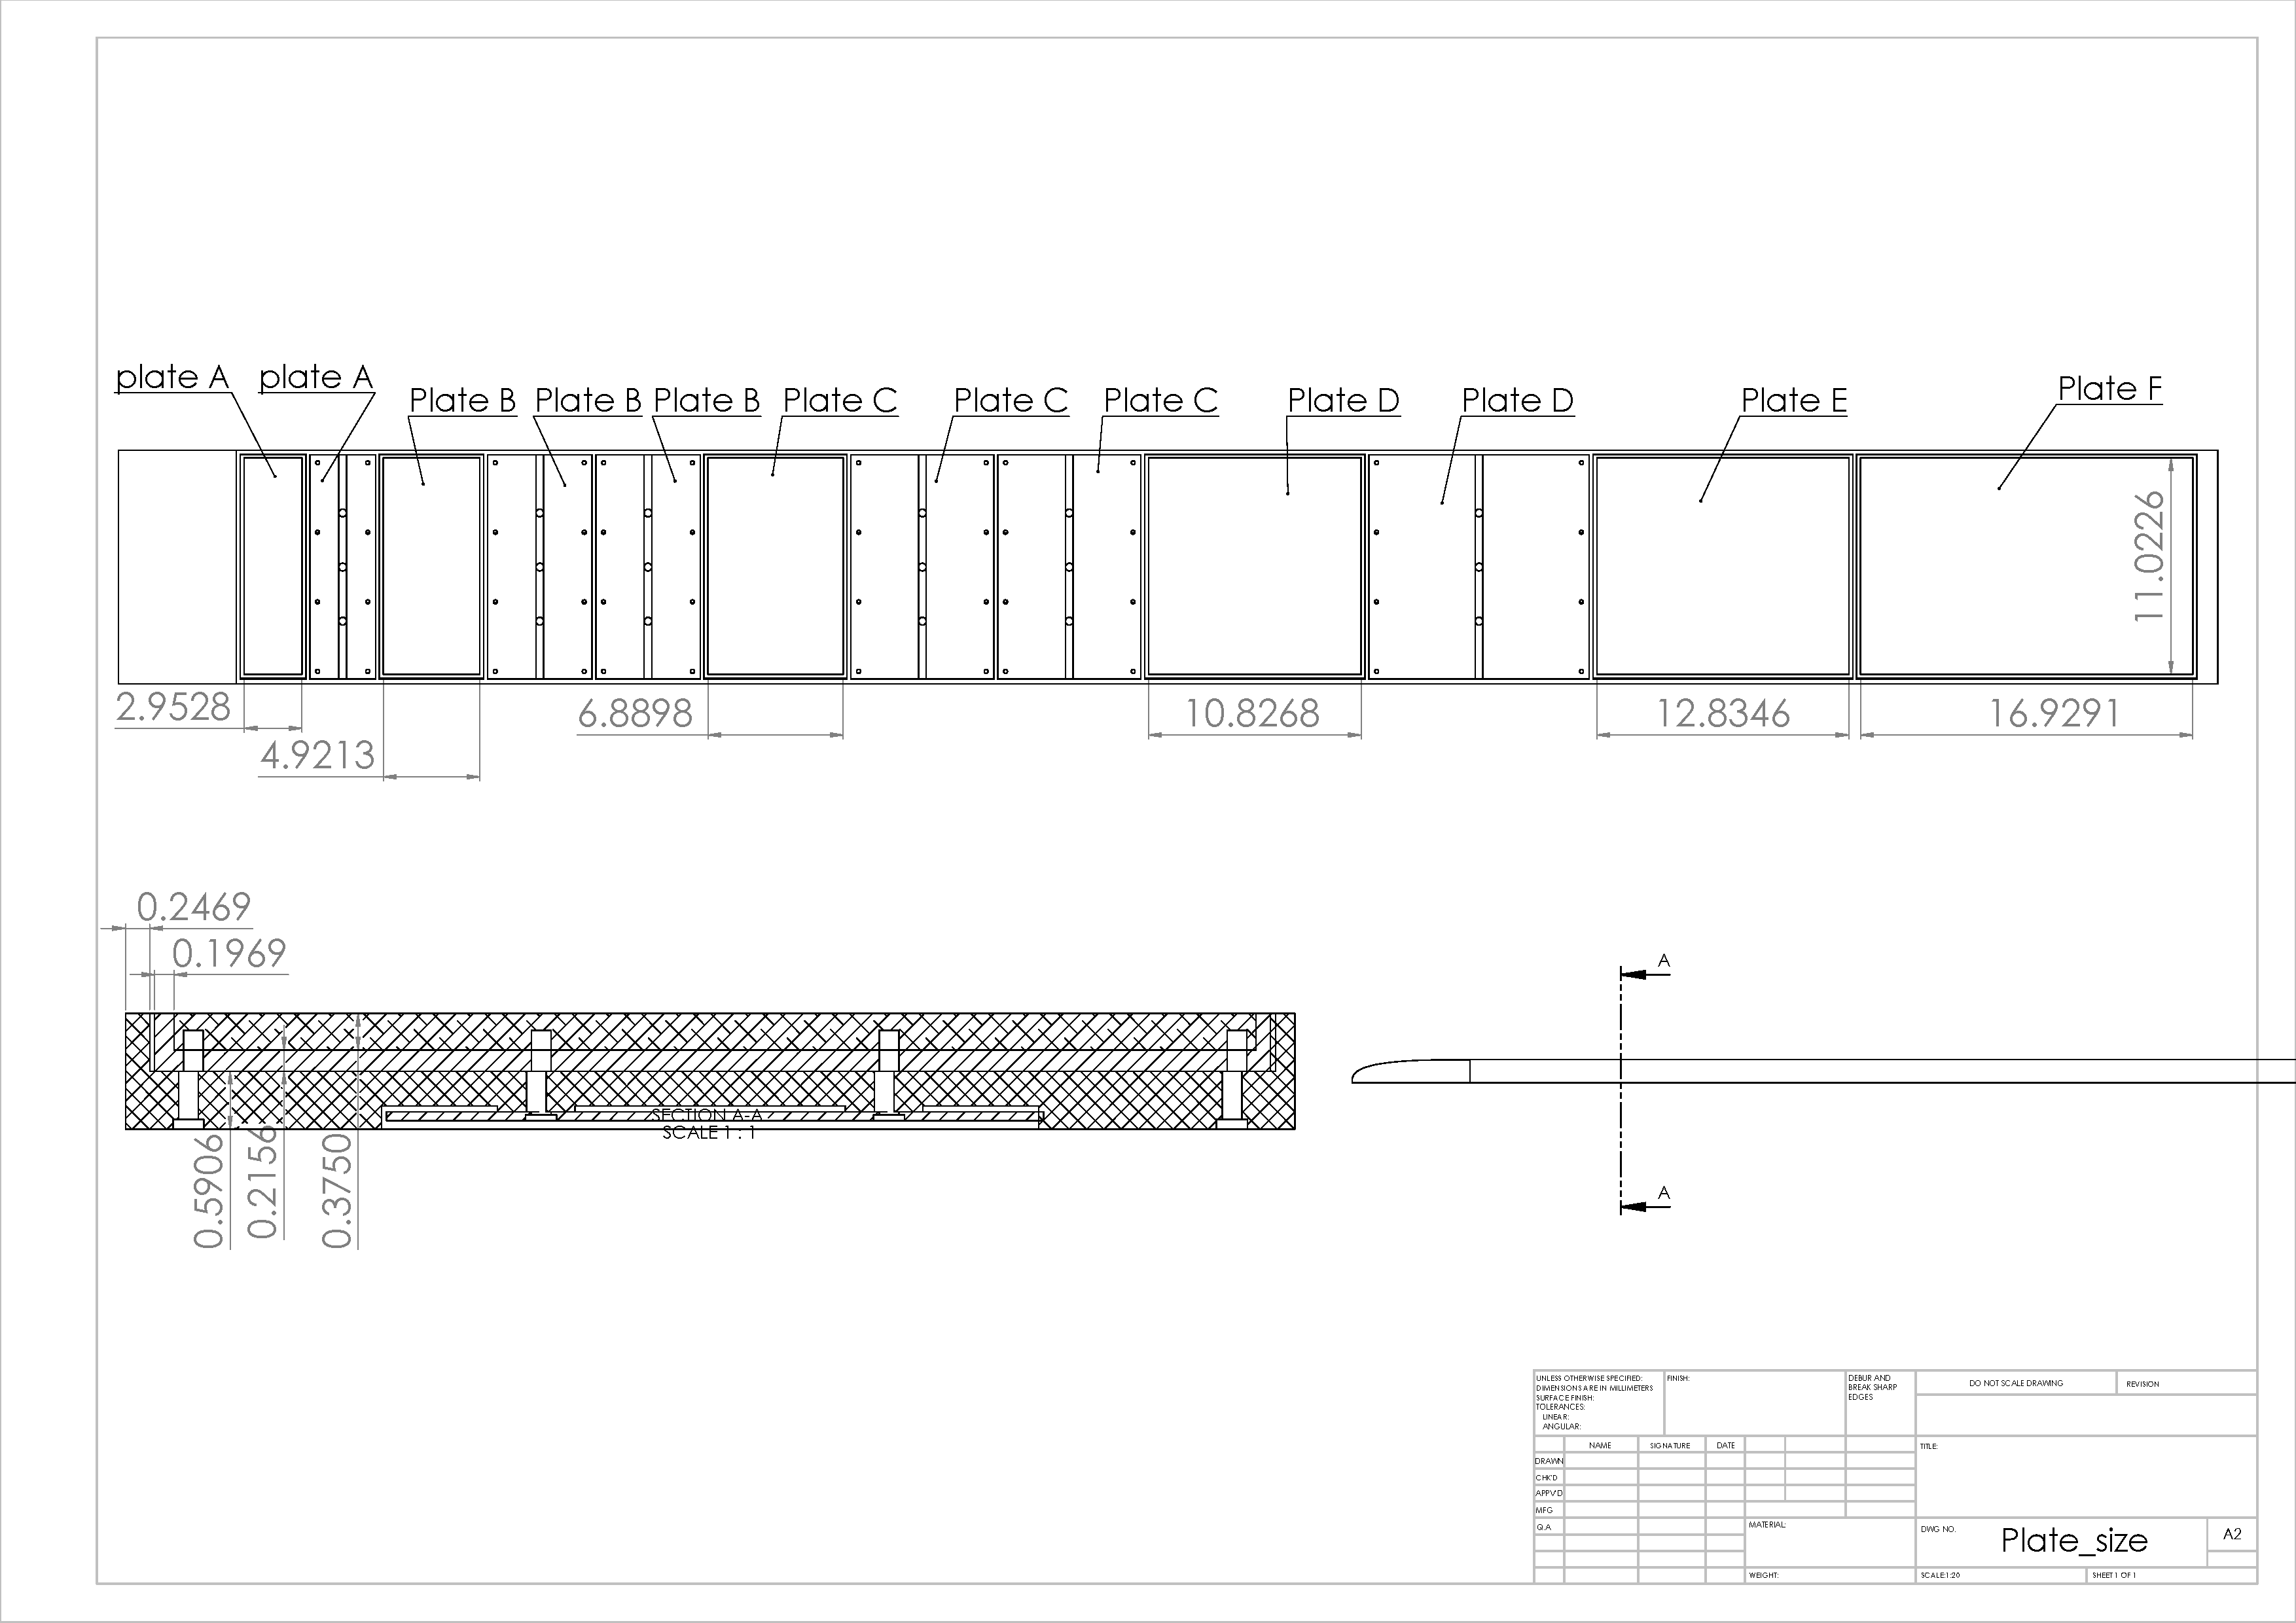
\includegraphics[scale=.3]{facility/drawings/Plate_size.PDF}
\caption{\footnotesize {\bf XX} } 
\end{figure}

%%%%%%%%%%%%%%%%%%%%%%%%%%%%%%%%%%%%%%%%%%%%%%%%%%
\clearpage
\subsection{Components A}

%components A
\begin{figure}[h!]
\centering
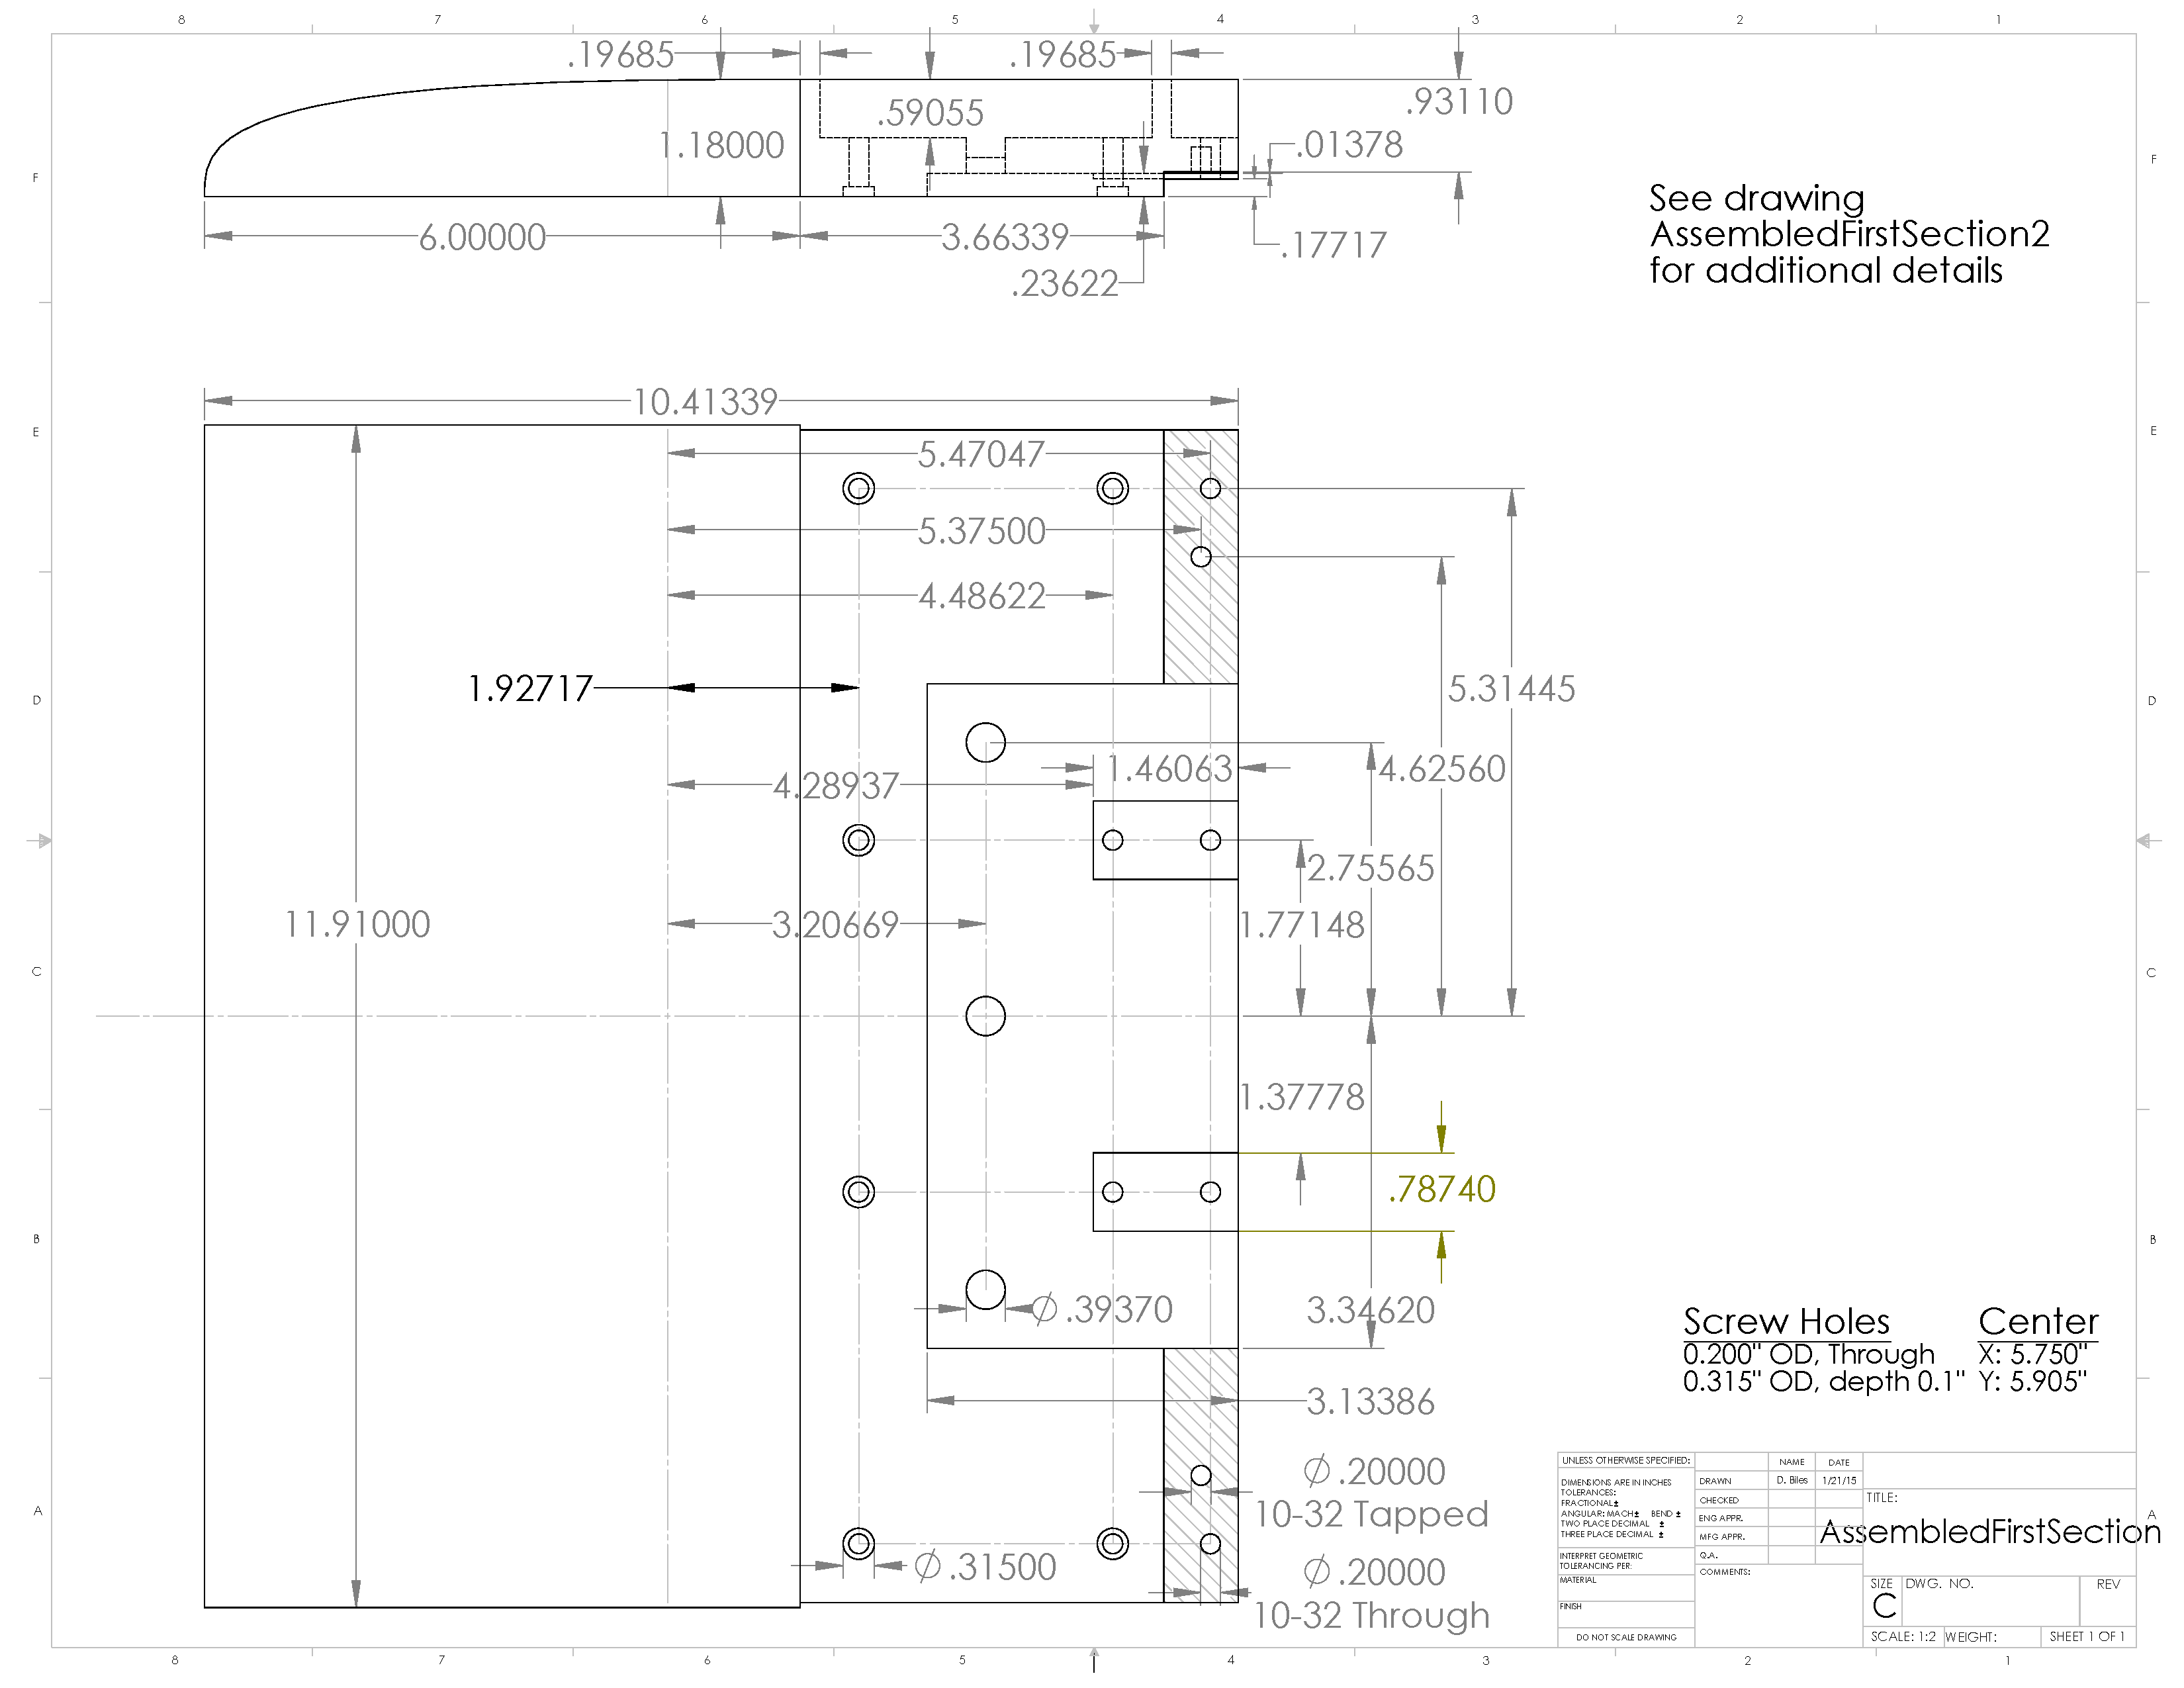
\includegraphics[scale=.2]{facility/drawings/AssembledFirstSection.PDF}
\caption{\footnotesize {\bf XX} } 
\end{figure}

\begin{figure}[h!]
\centering
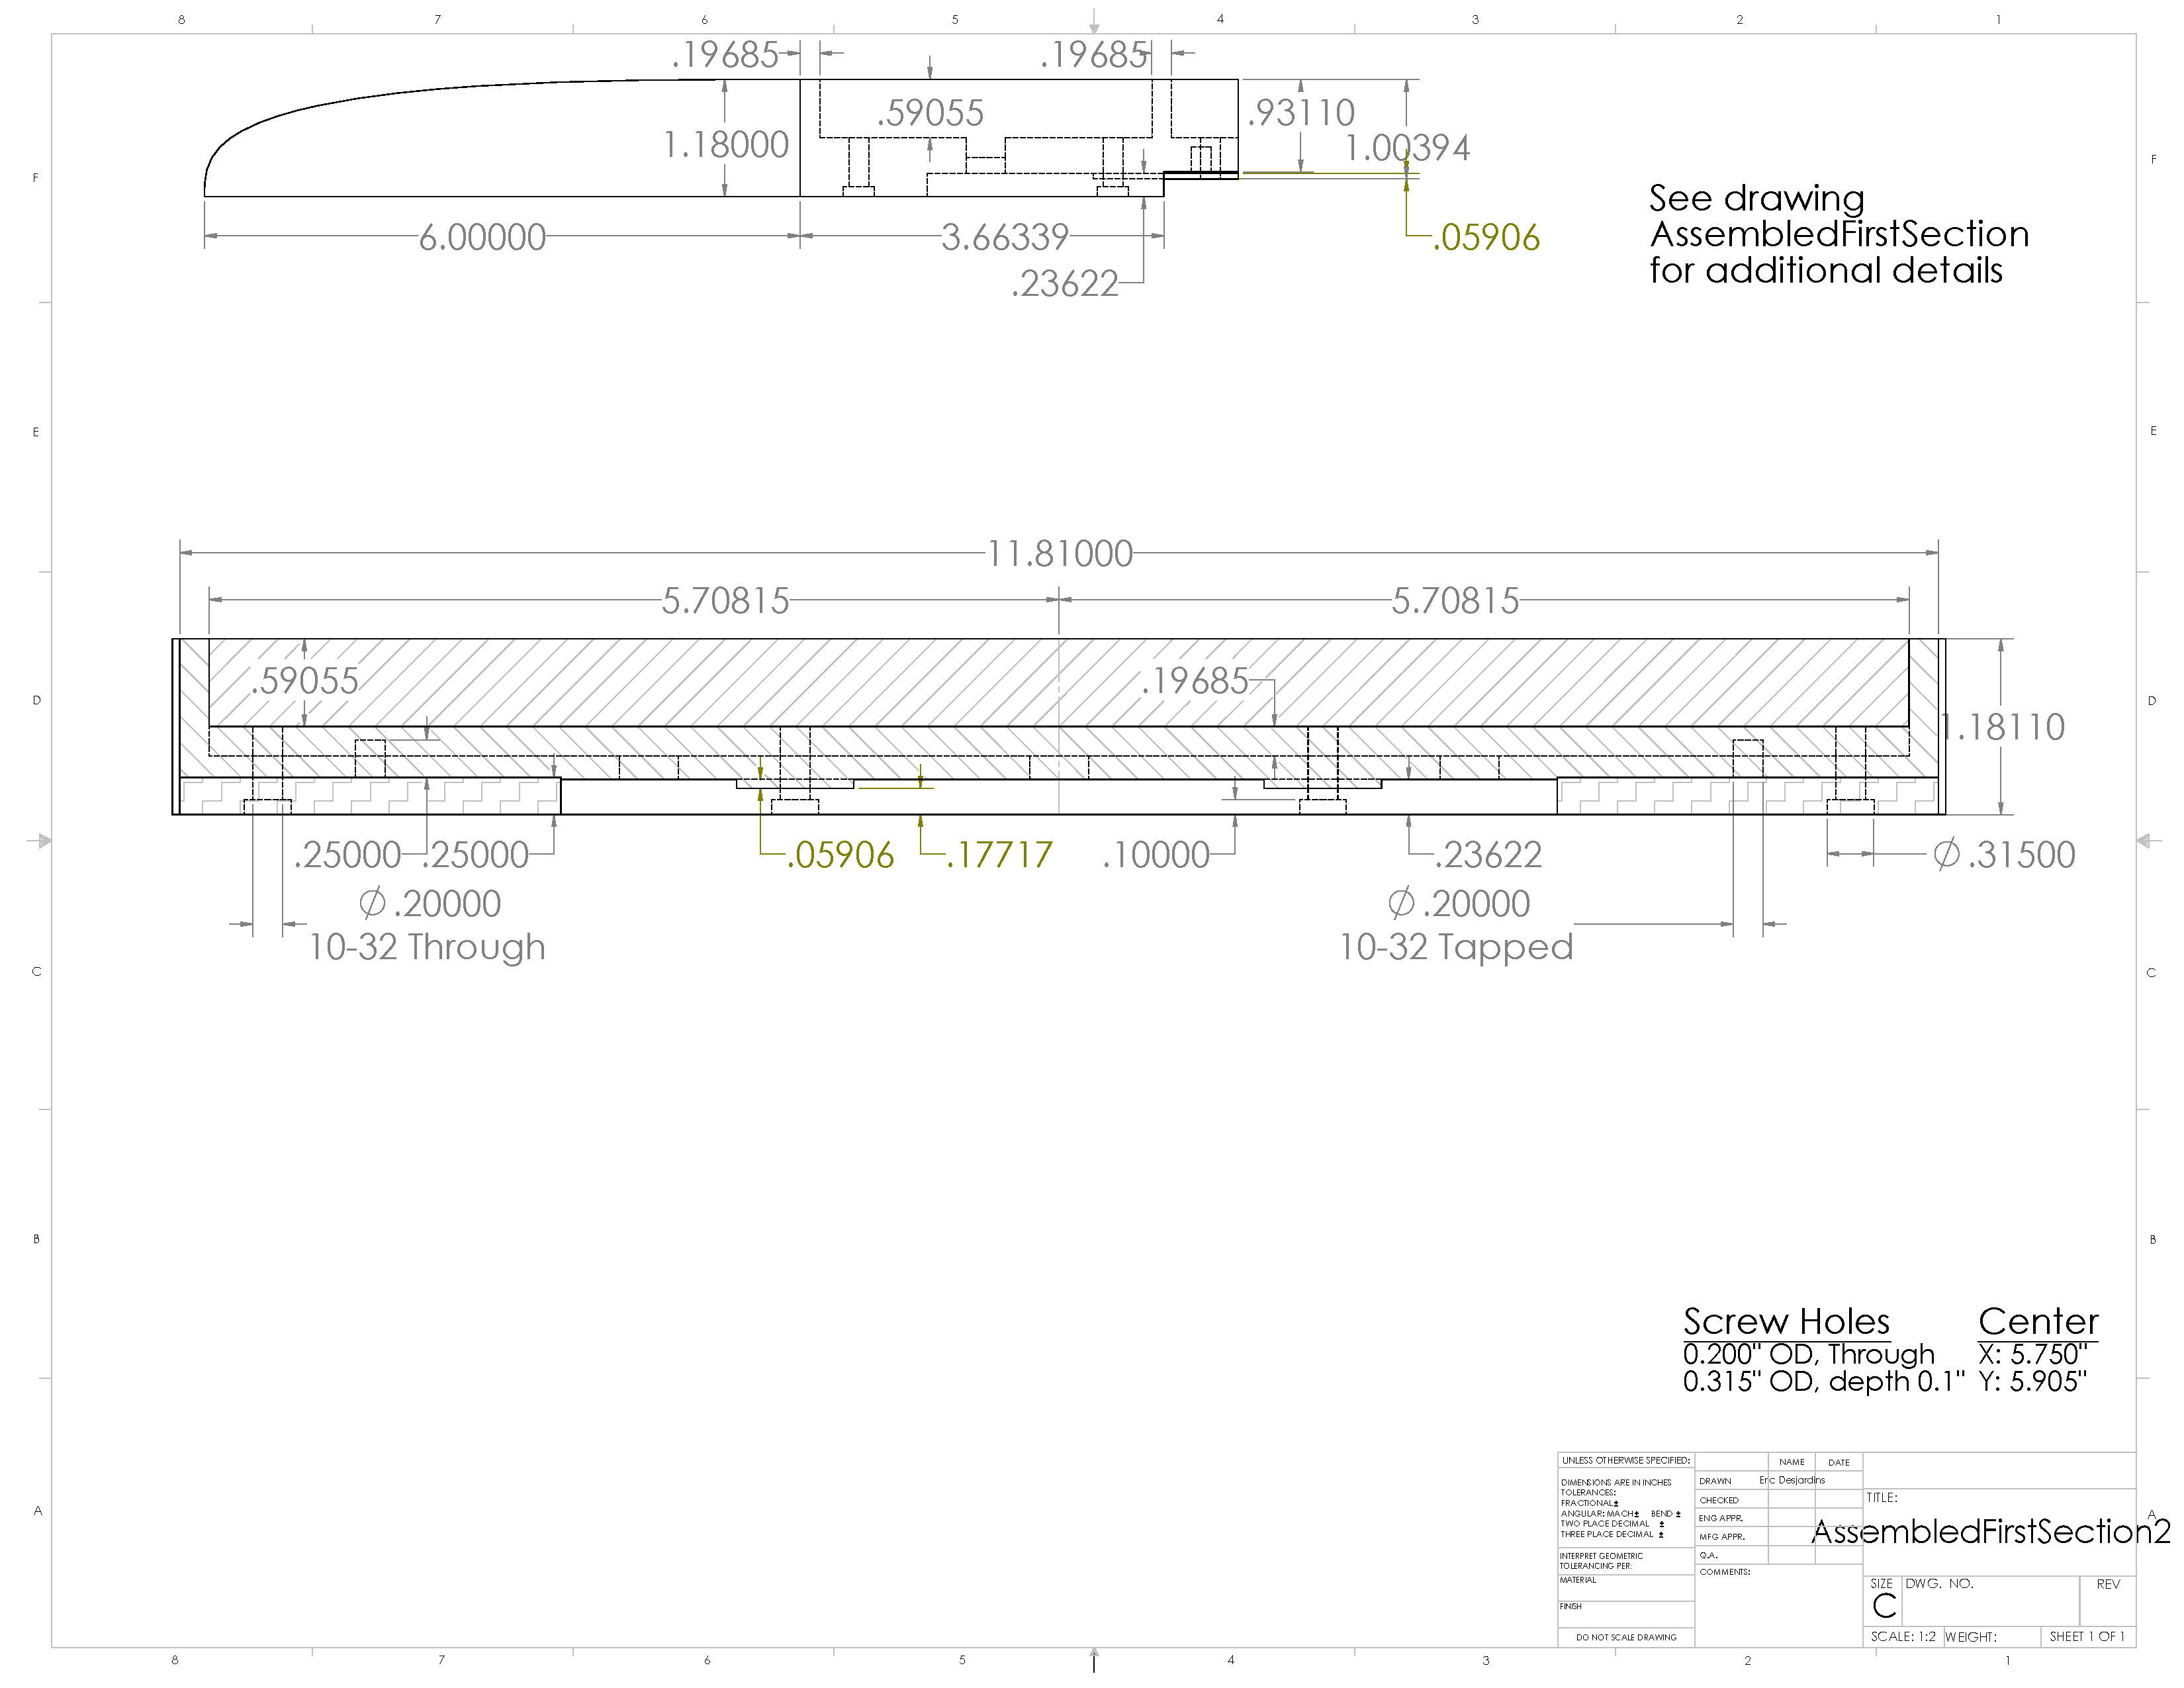
\includegraphics[scale=.2]{facility/drawings/AssembledFirstSection2.PDF}
\caption{\footnotesize {\bf XX} } 
\end{figure}

\begin{figure}[h!]
\centering
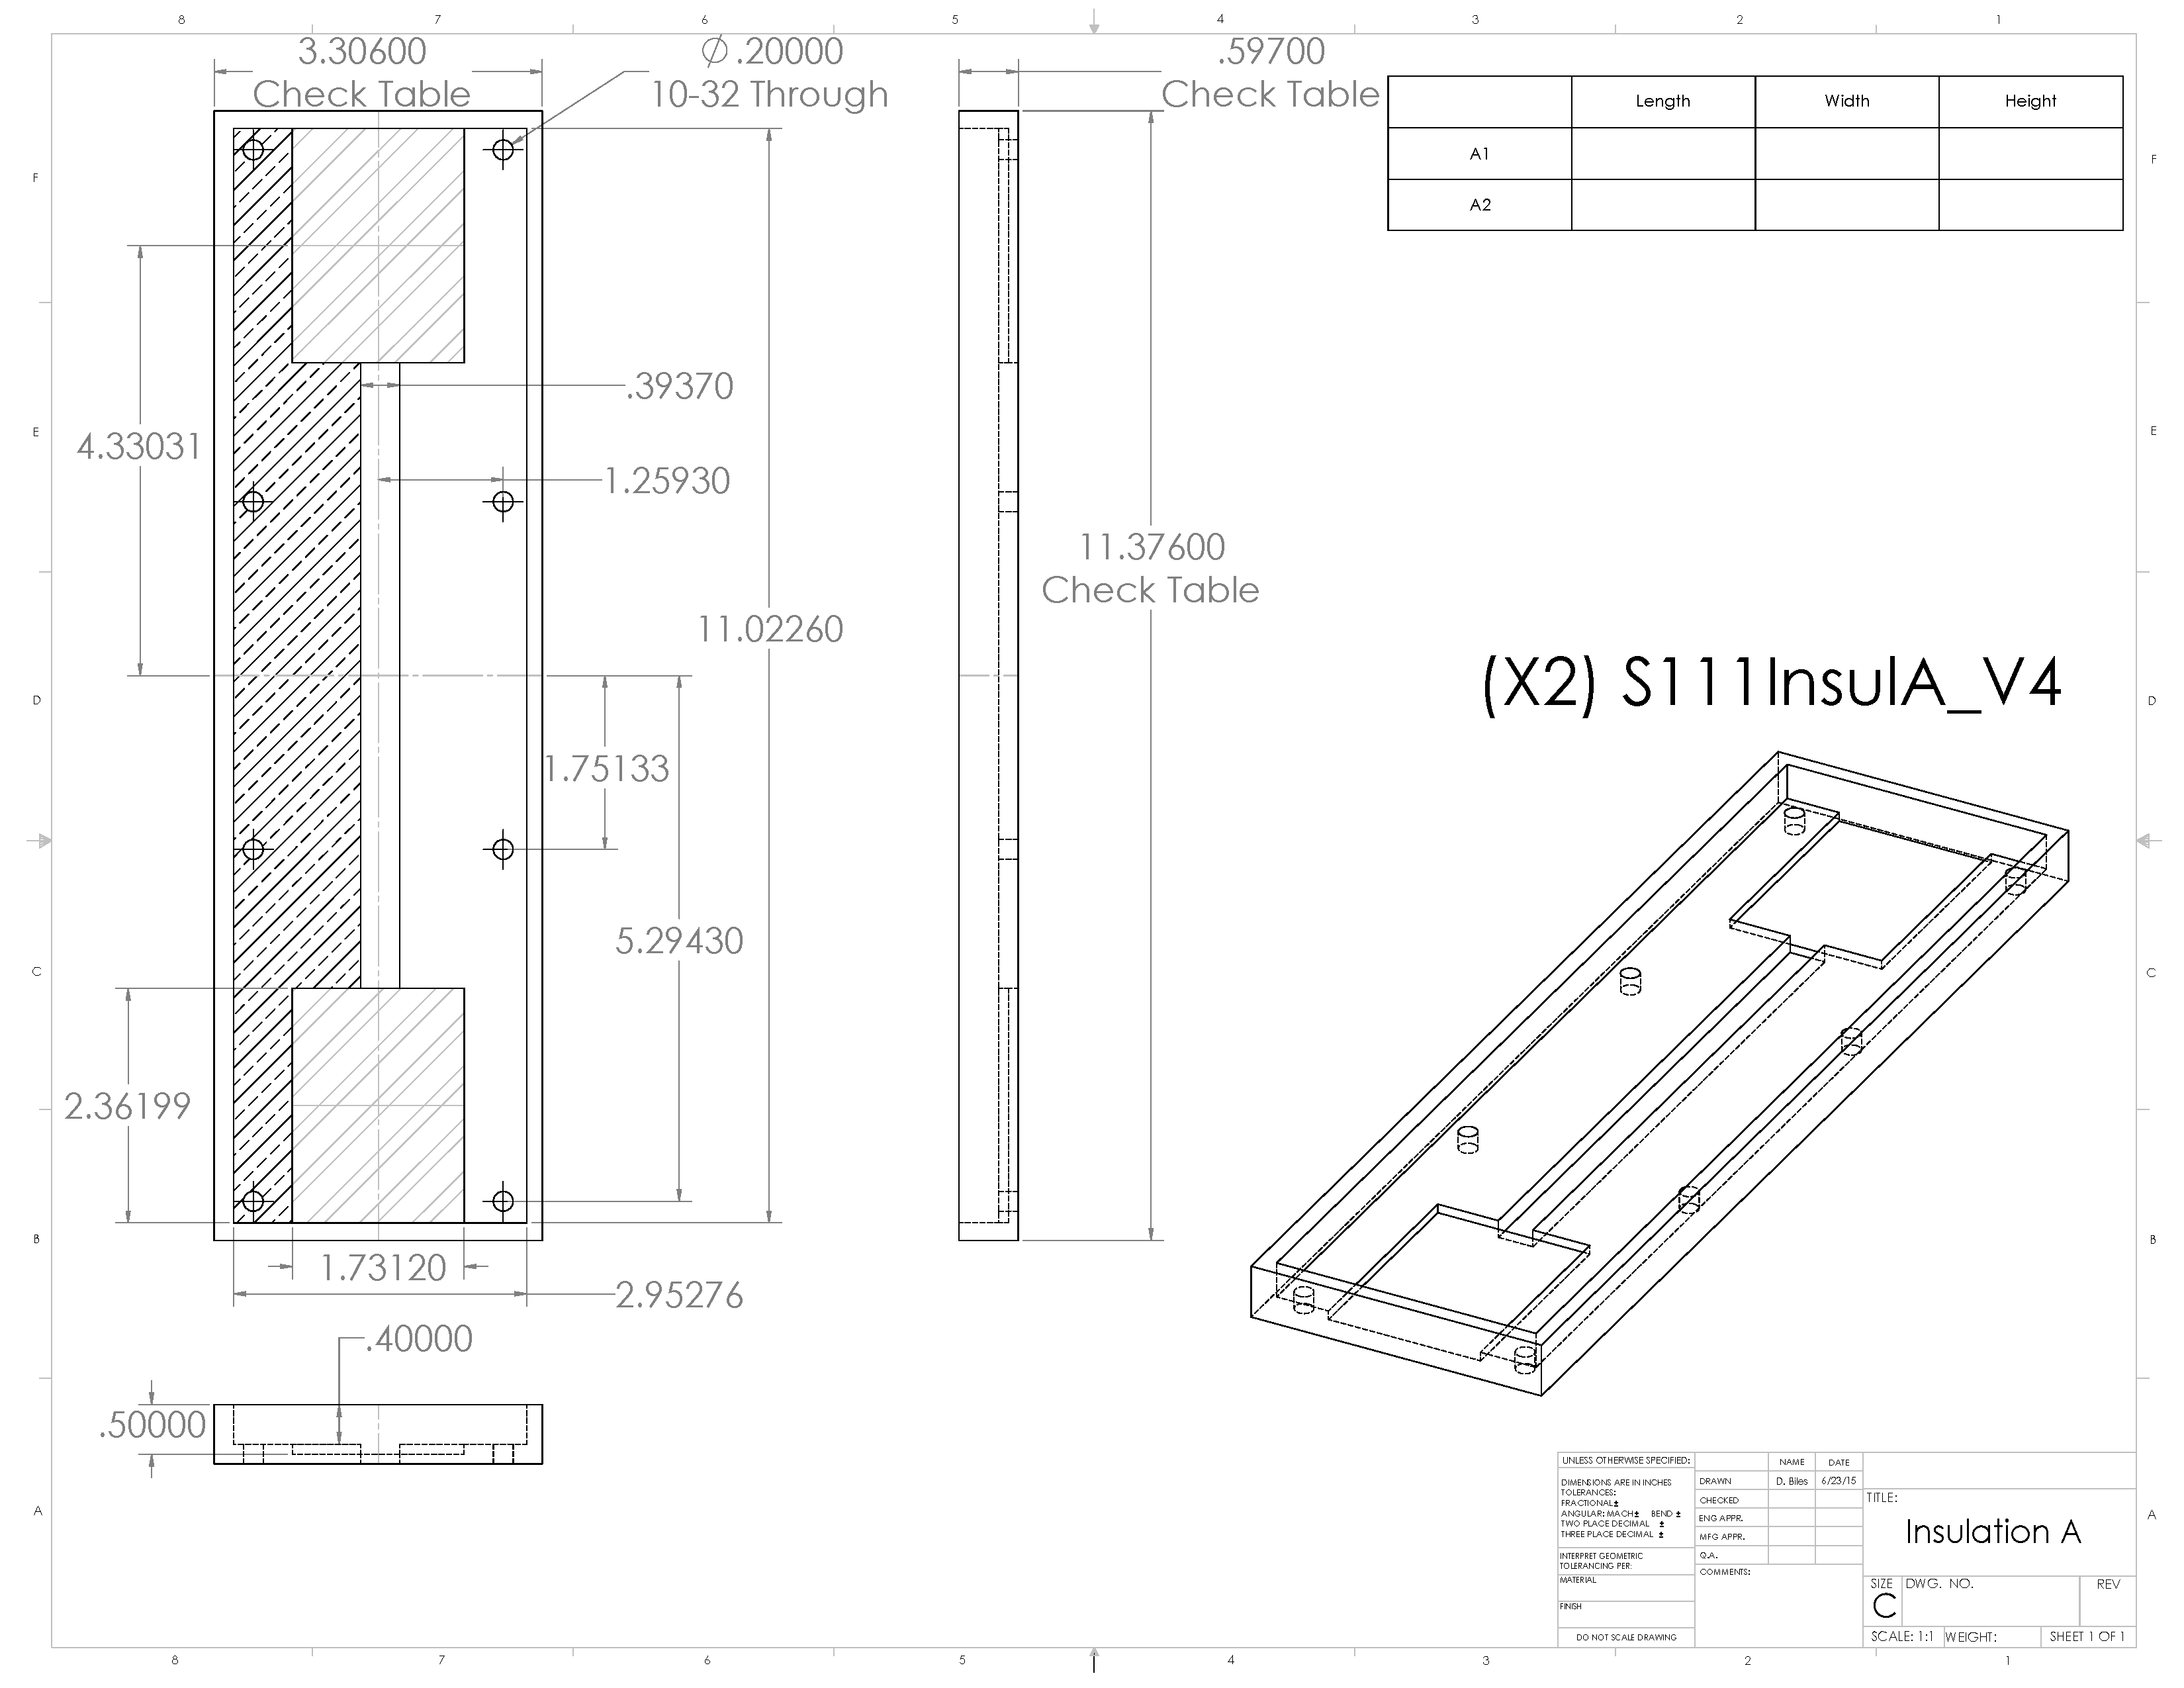
\includegraphics[scale=.2]{facility/drawings/Insulation_A.PDF}
\caption{\footnotesize {\bf XX} } 
\end{figure}

\begin{figure}[h!]
\centering
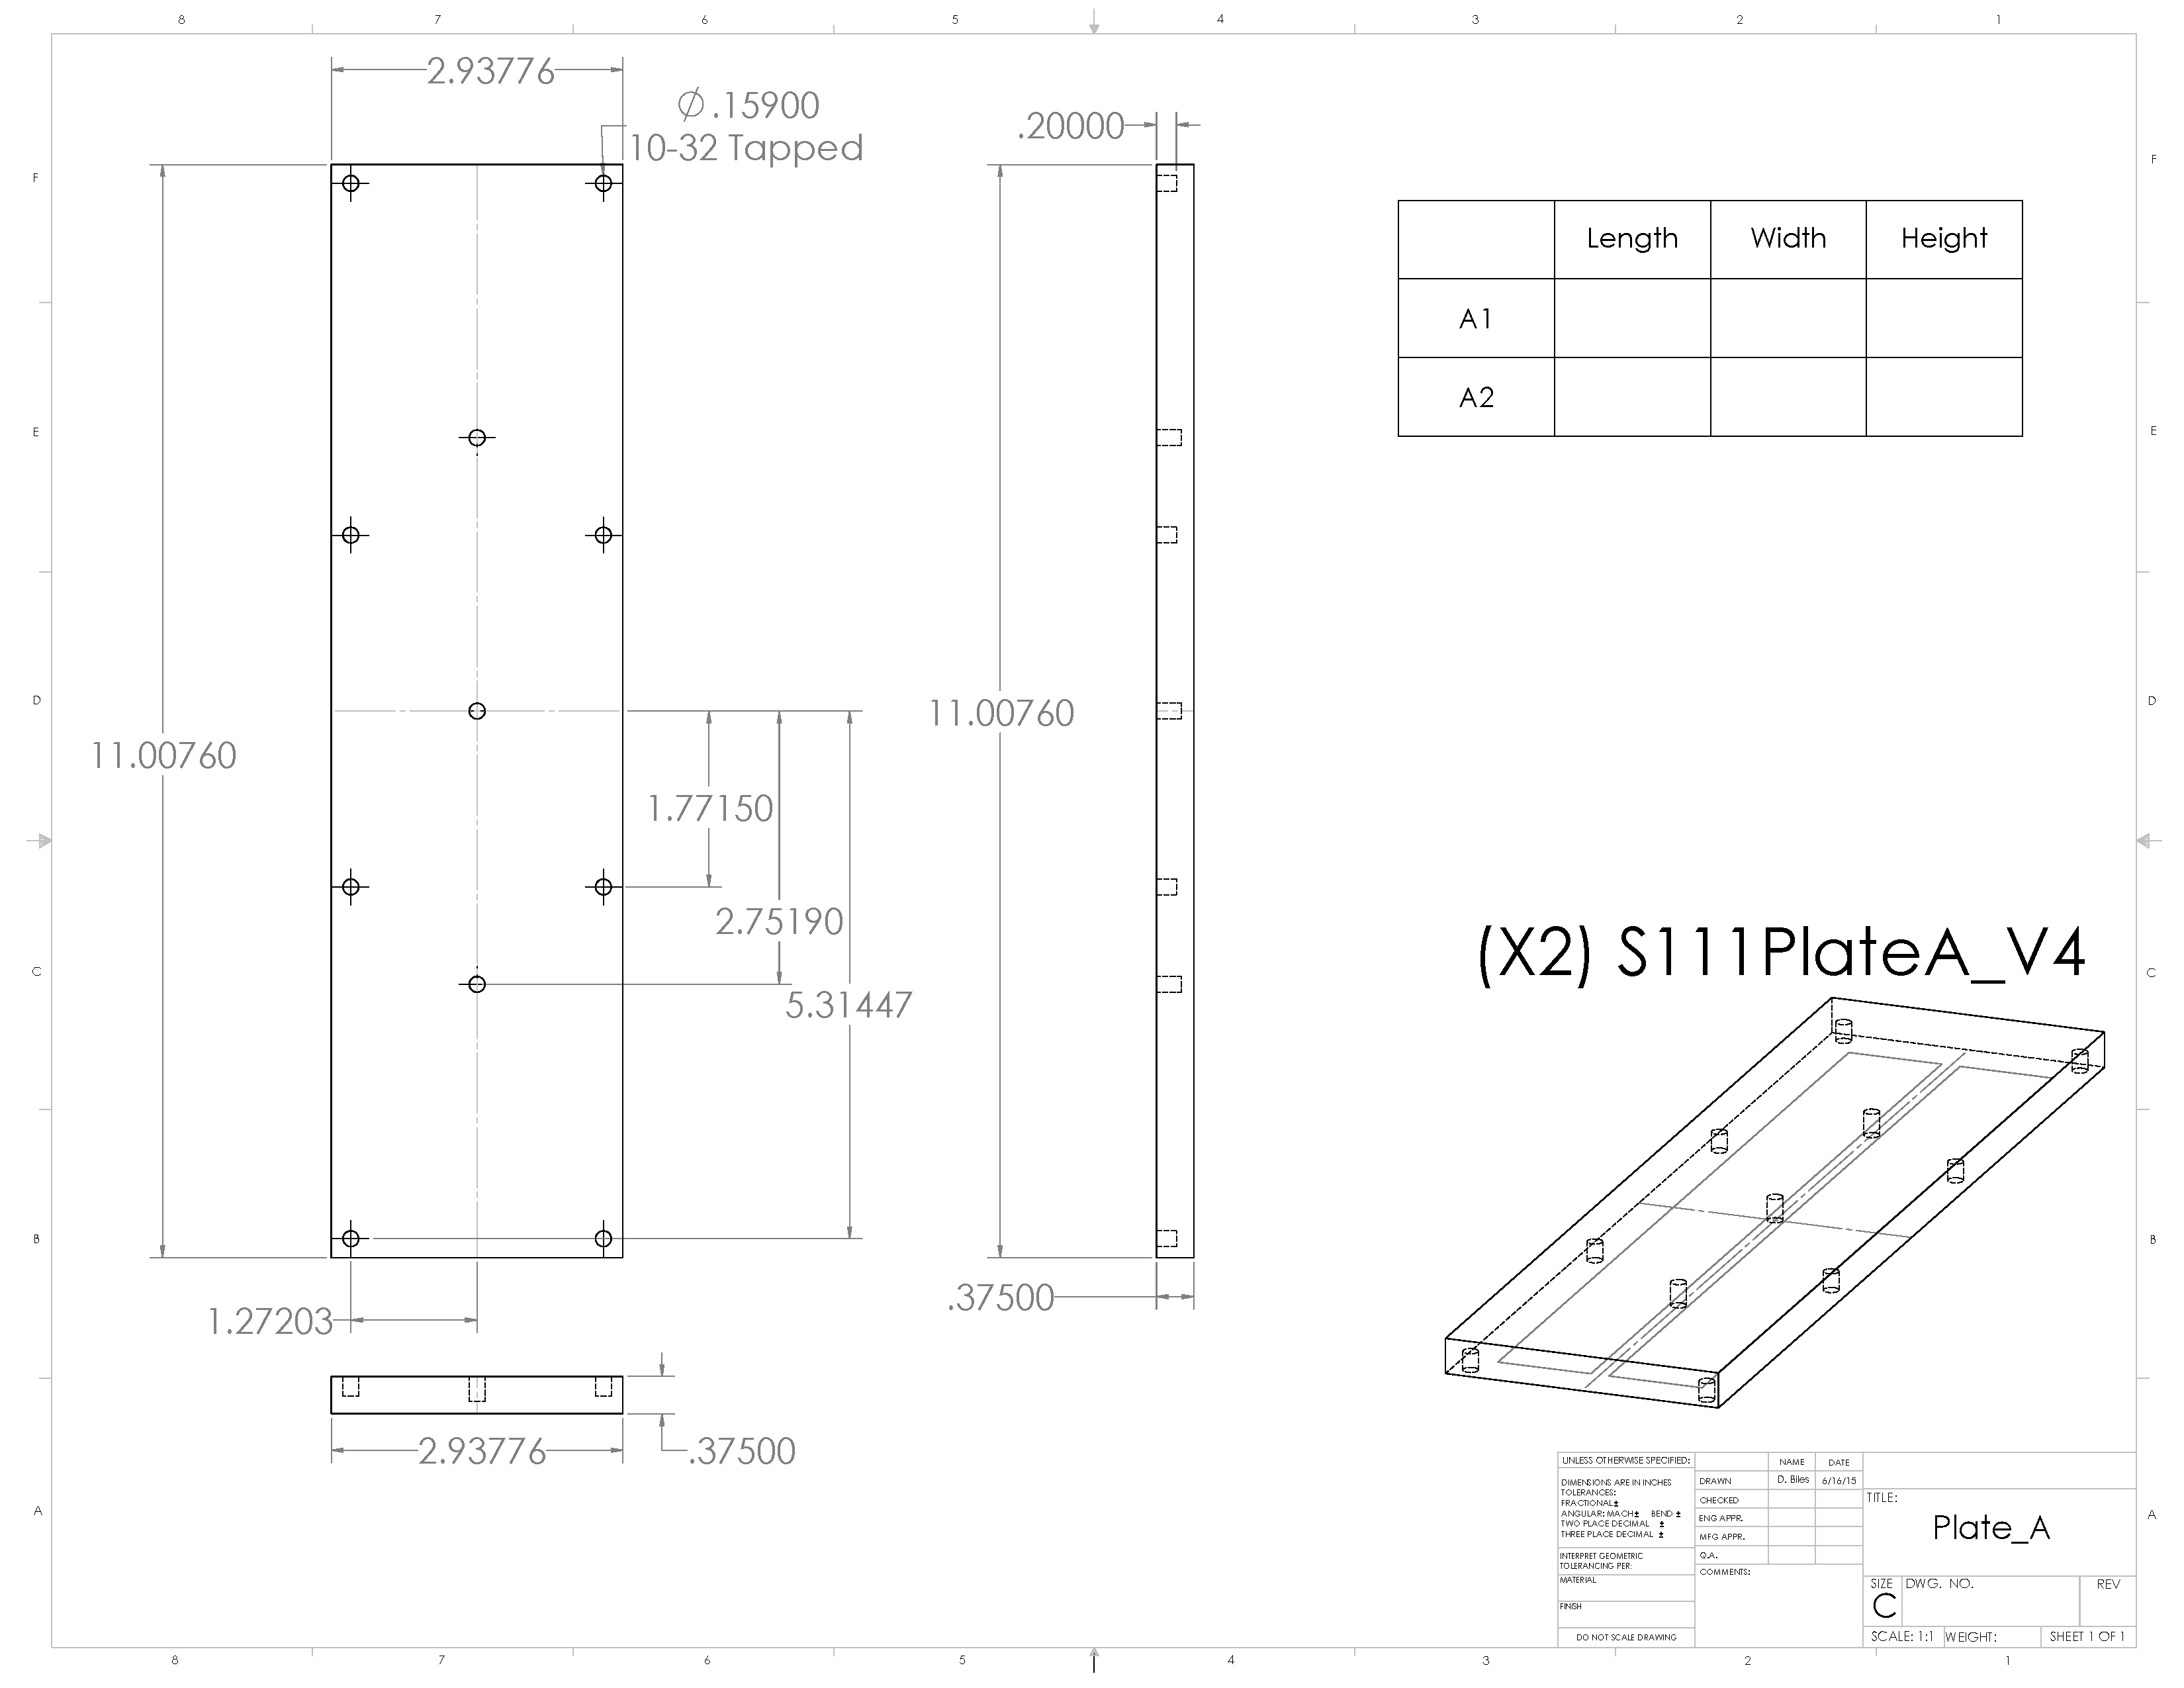
\includegraphics[scale=.2]{facility/drawings/Plate_A.PDF}
\caption{\footnotesize {\bf XX} } 
\end{figure}


\begin{figure}[h!]
  \begin{center}
  {\subfigcapskip = 5pt \subfigcapmargin = -12pt \subfigure[]{\label{fig:edge-a}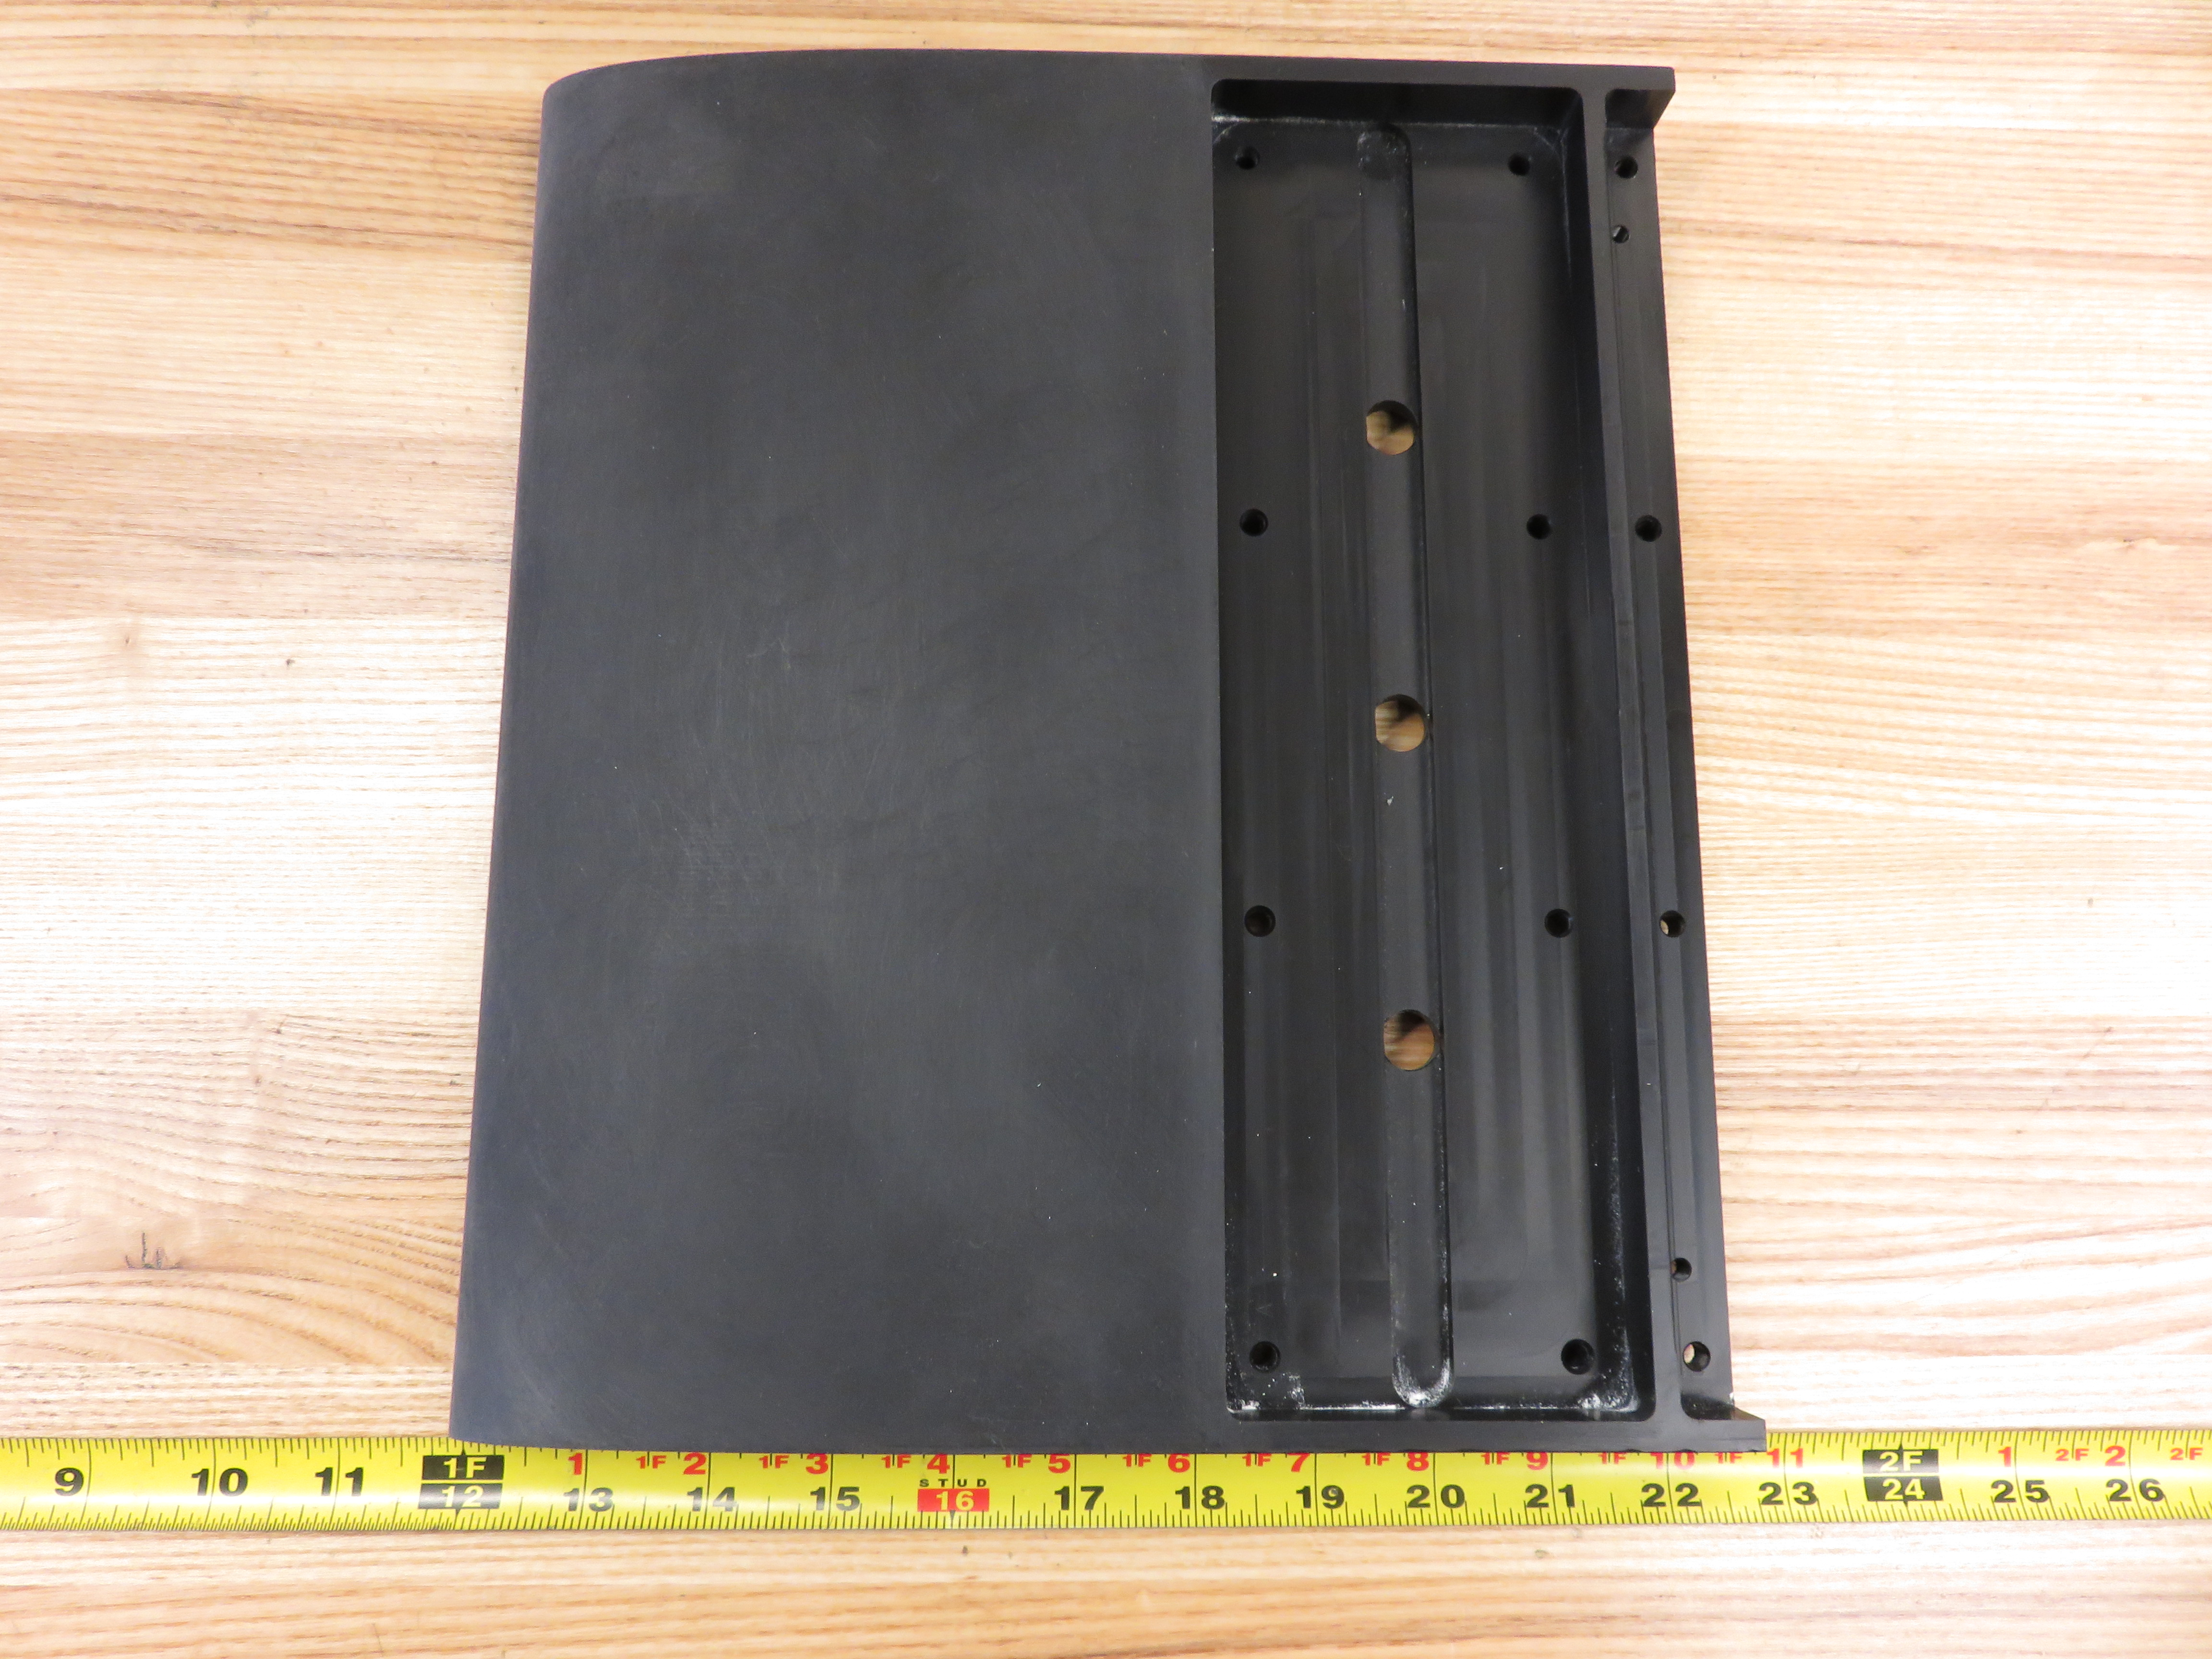
\includegraphics[scale=0.2]{facility/MachinedParts/A_meas_v2.JPG}}}
   {\subfigcapskip = 5pt \subfigcapmargin = -12pt  \subfigure[]{\label{fig:edge-b}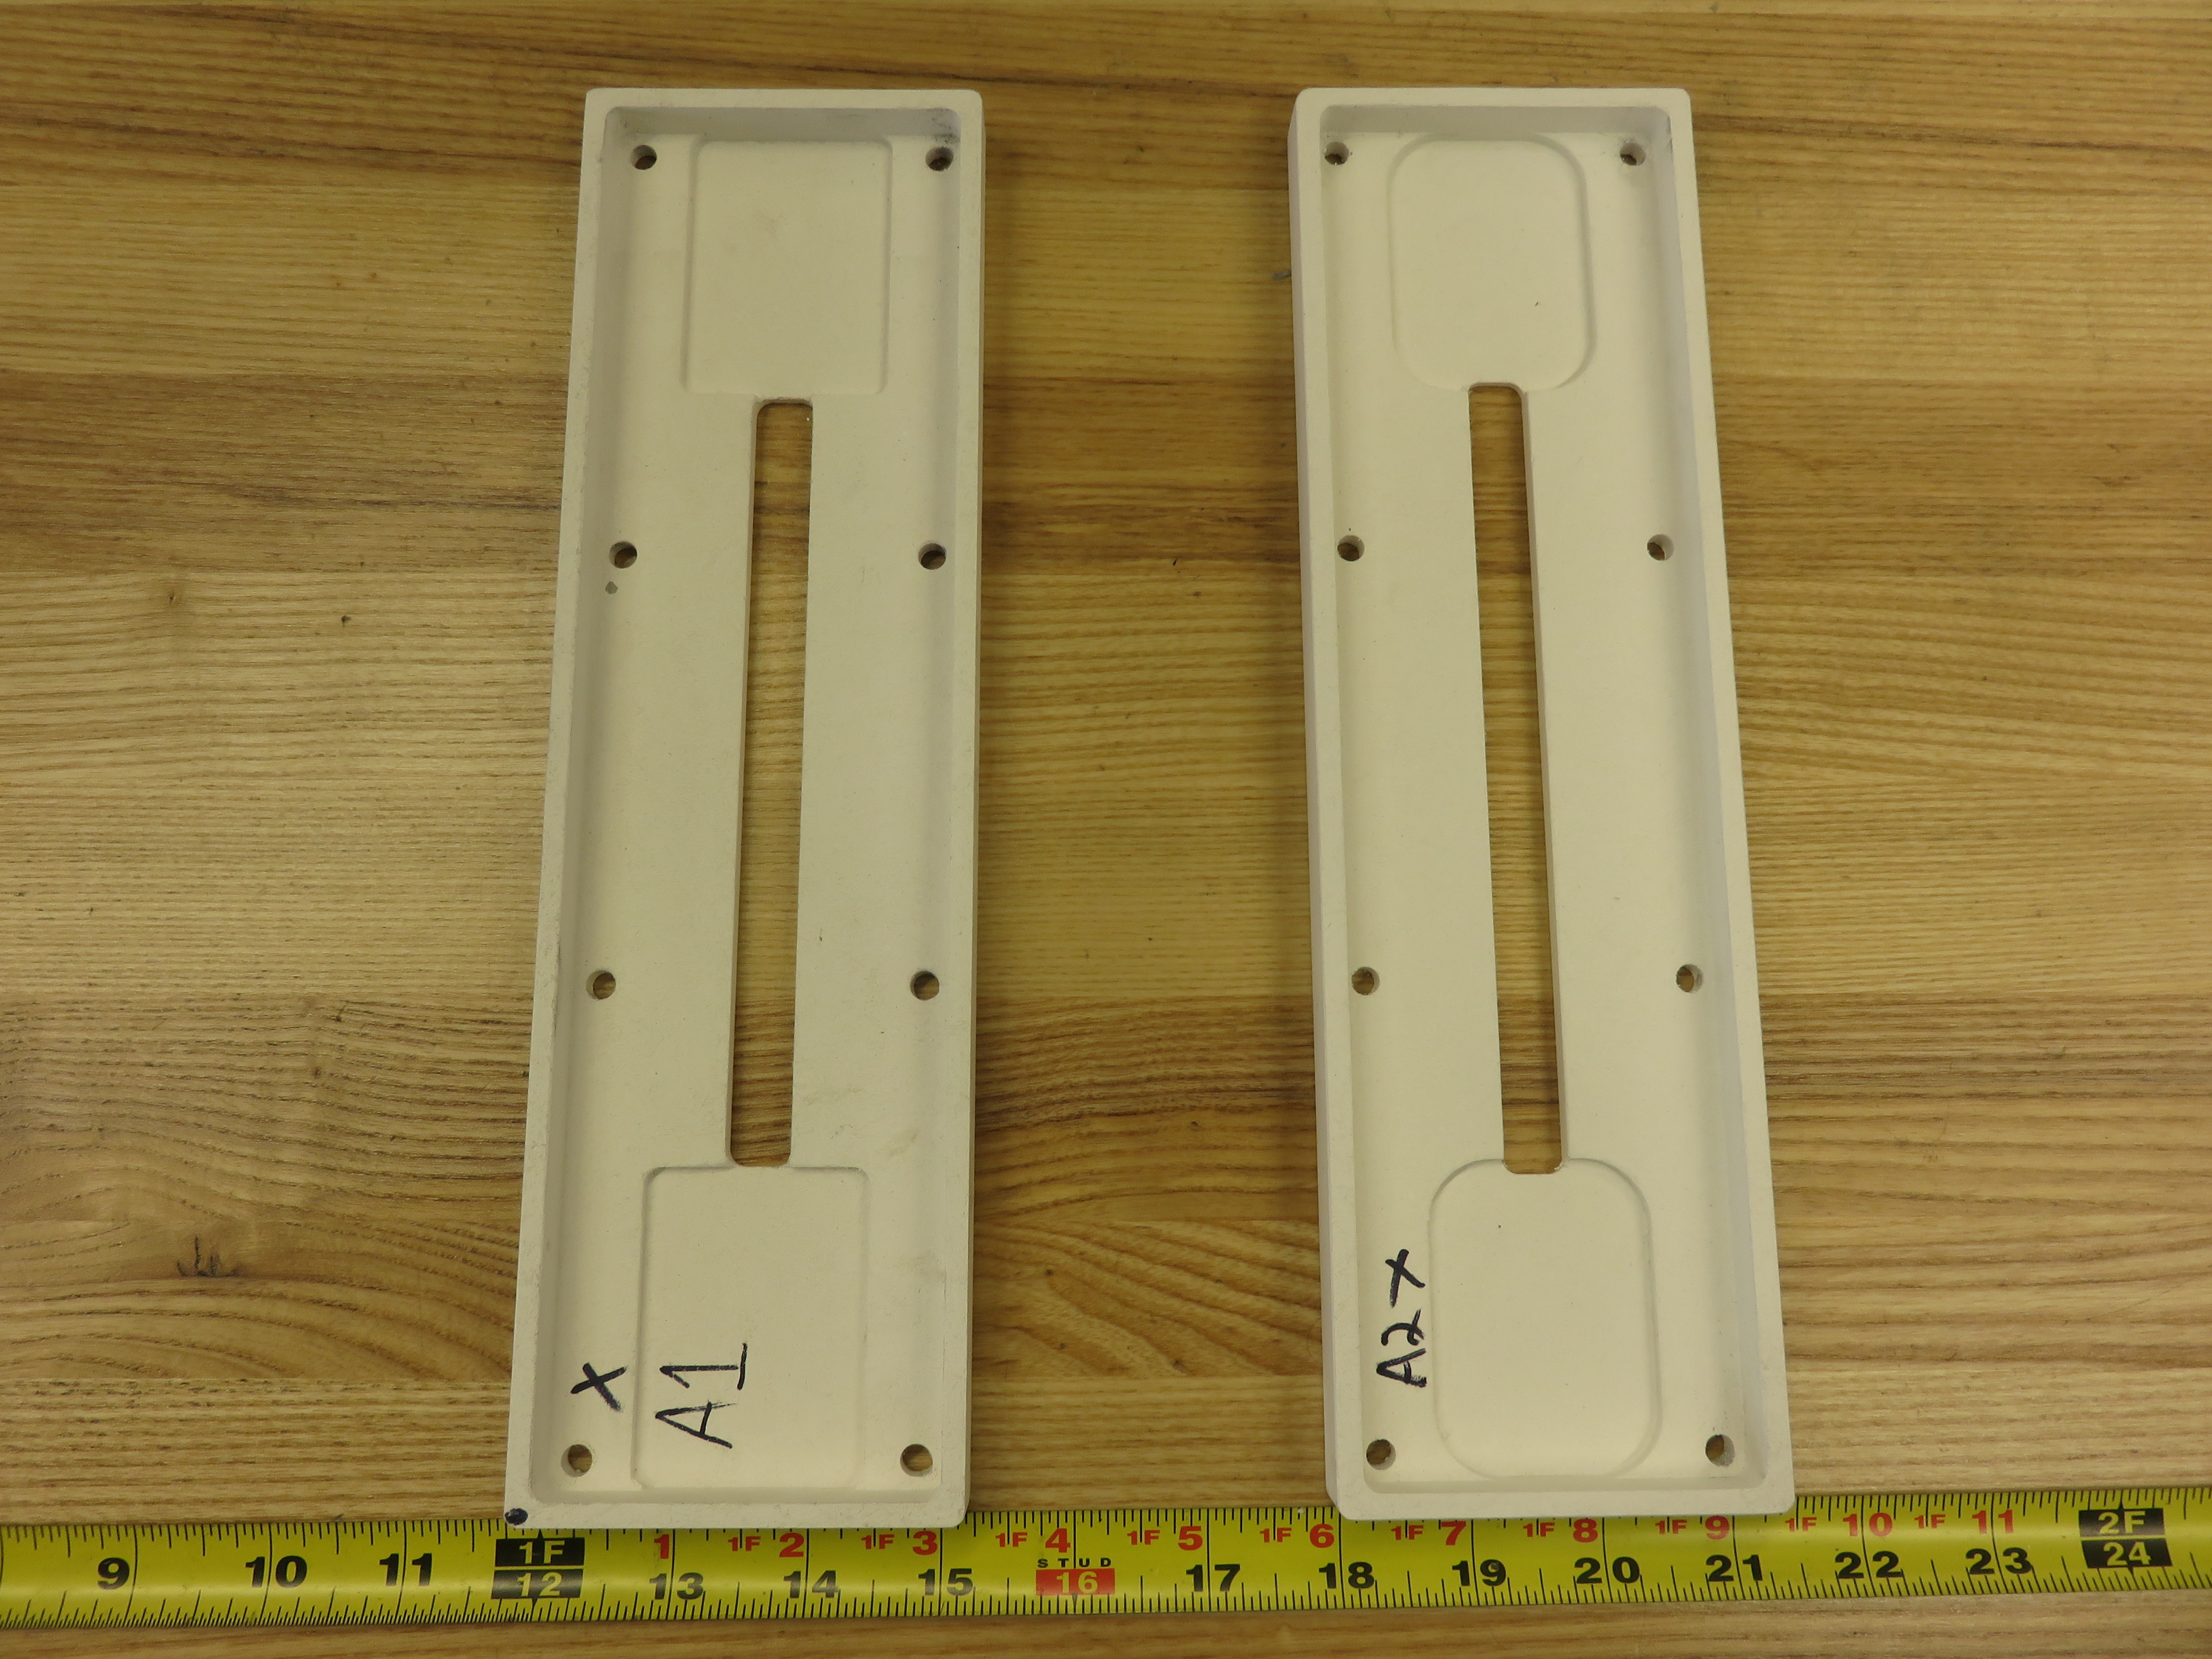
\includegraphics[scale=0.2]{facility/MachinedParts/A_insul_v2.JPG}}}
  \end{center}
\caption{(a) insulation (b) frame. } 
\end{figure}


%%%%%%%%%%%%%%%%%%%%%%%%%%%%%%%%%%%%%%%%%%%%%%%%%%%%%%
\clearpage
\subsection{Components B}
Input text description?\\

%components B
\begin{figure}[h!]
\centering
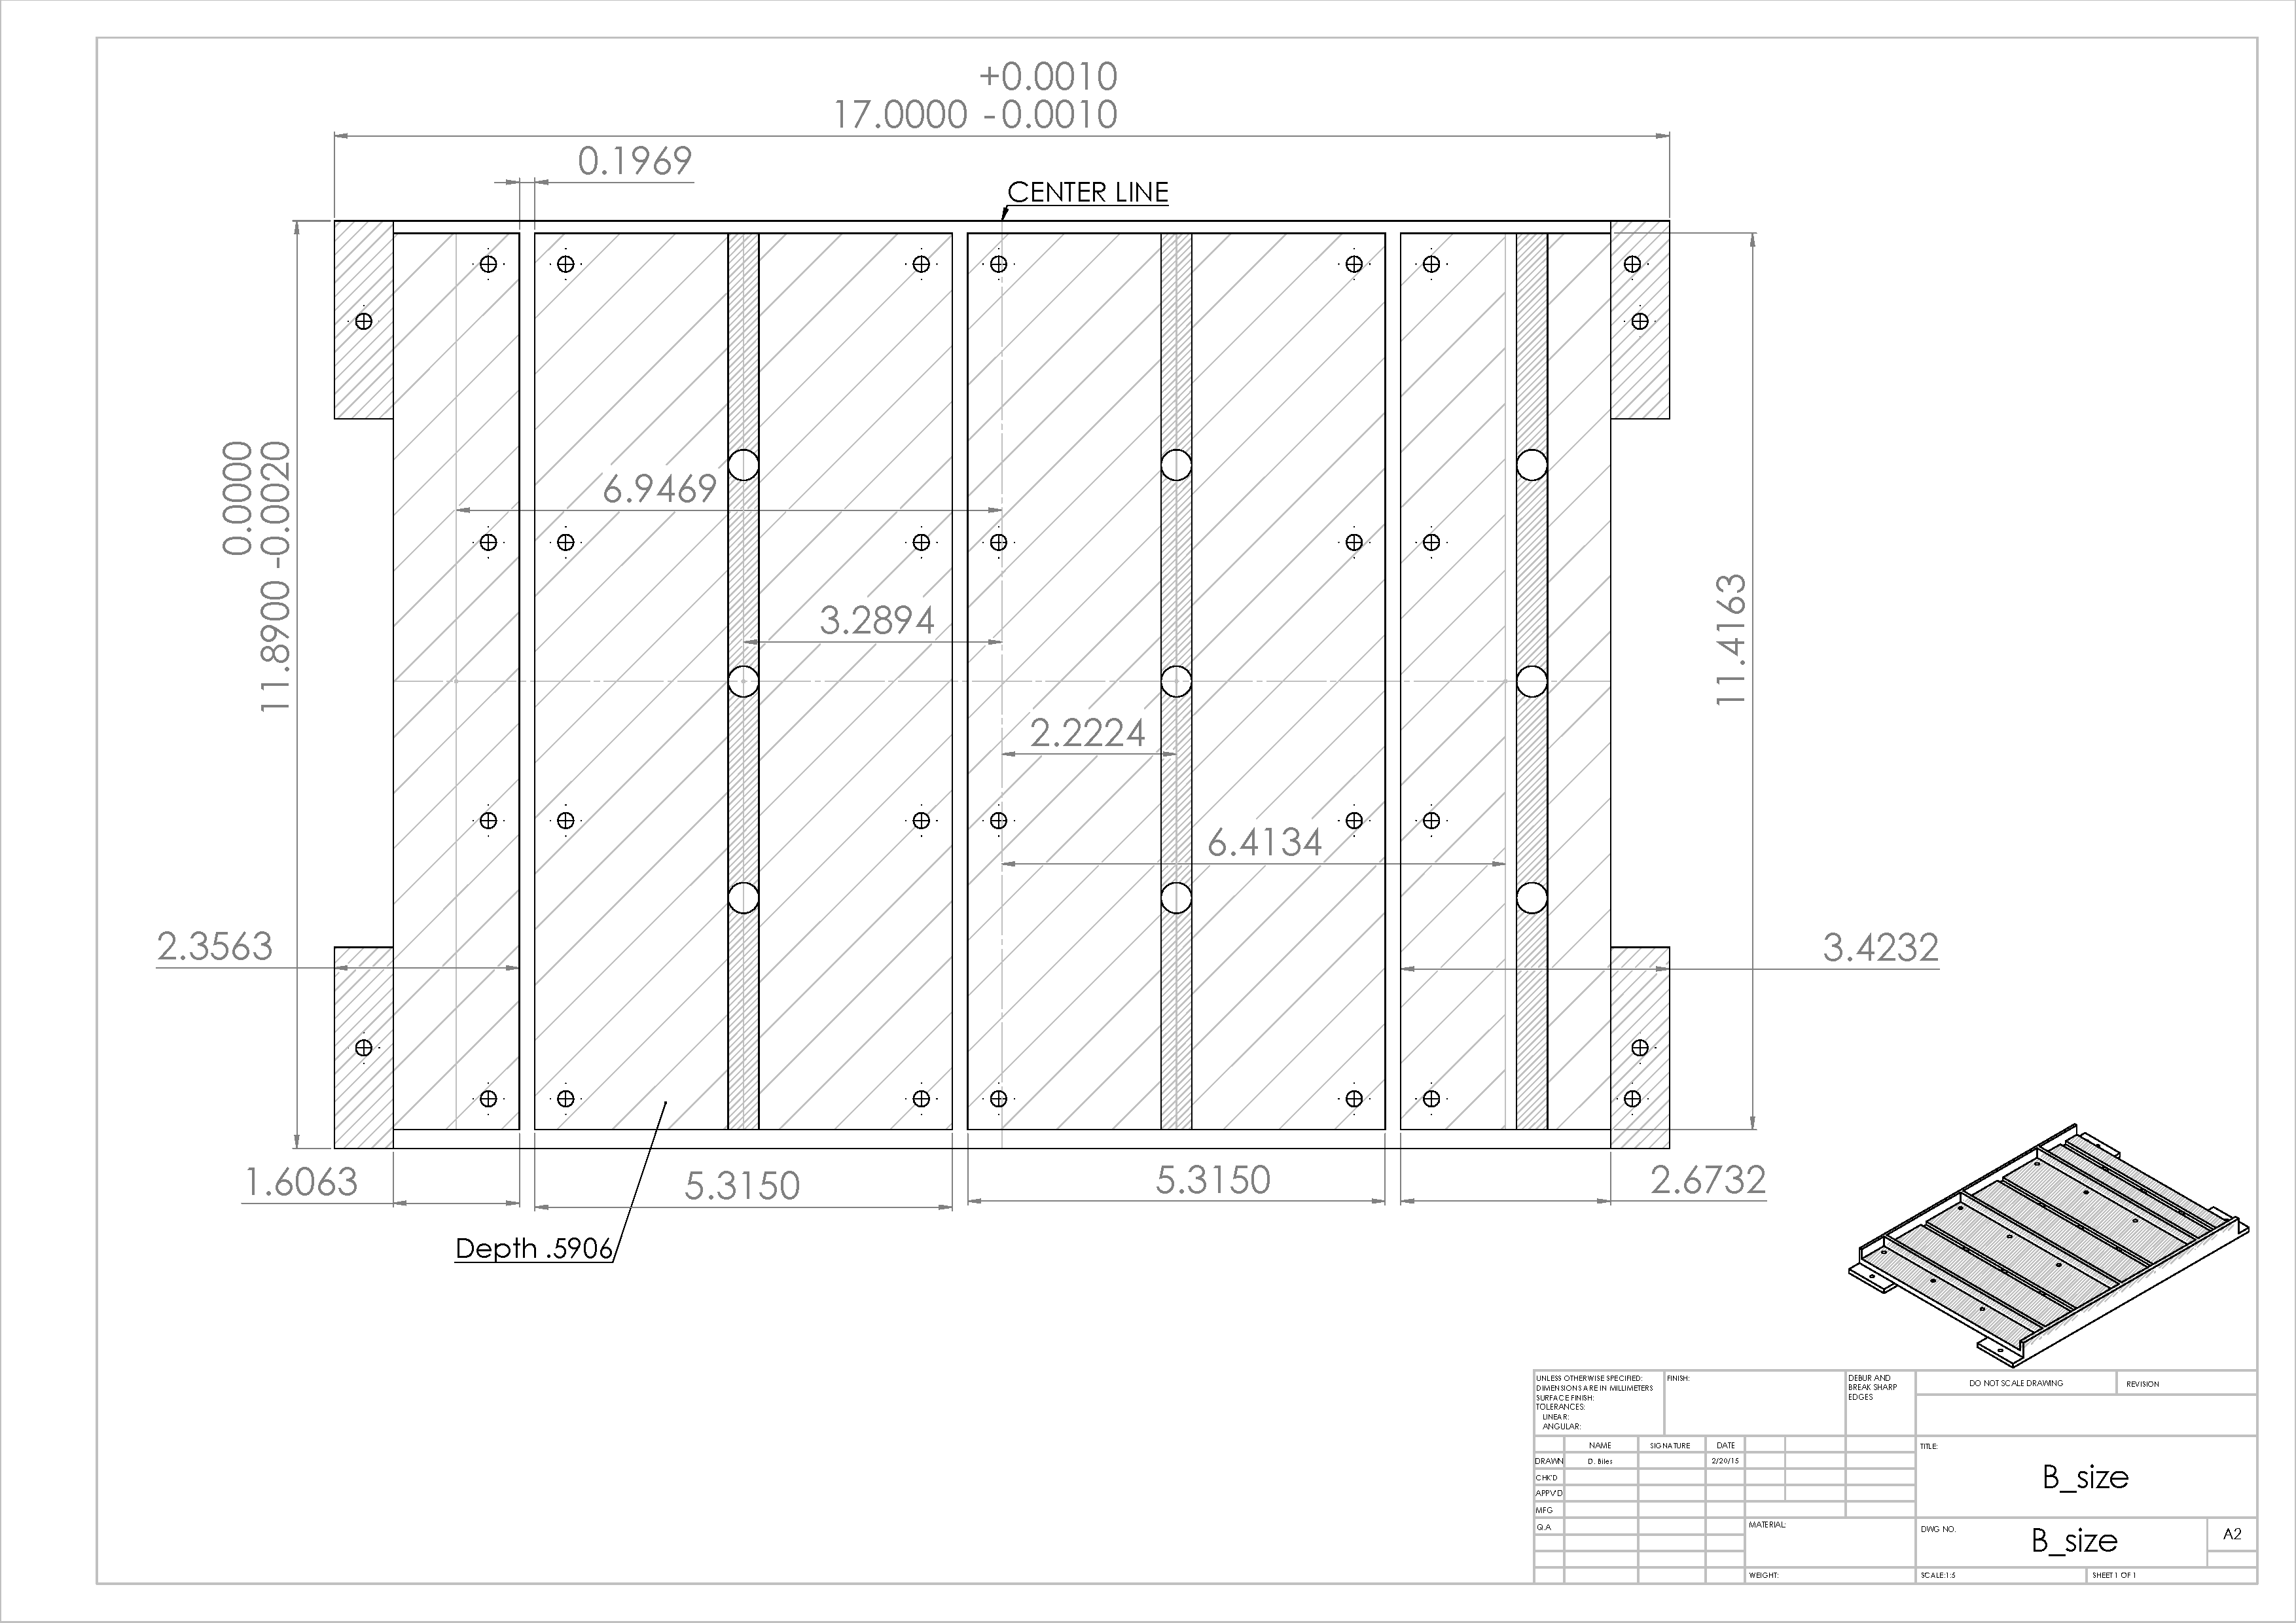
\includegraphics[scale=.2]{facility/drawings/B_size.PDF}
\caption{\footnotesize {\bf XX} } 
\end{figure}

\begin{figure}[h!]
\centering
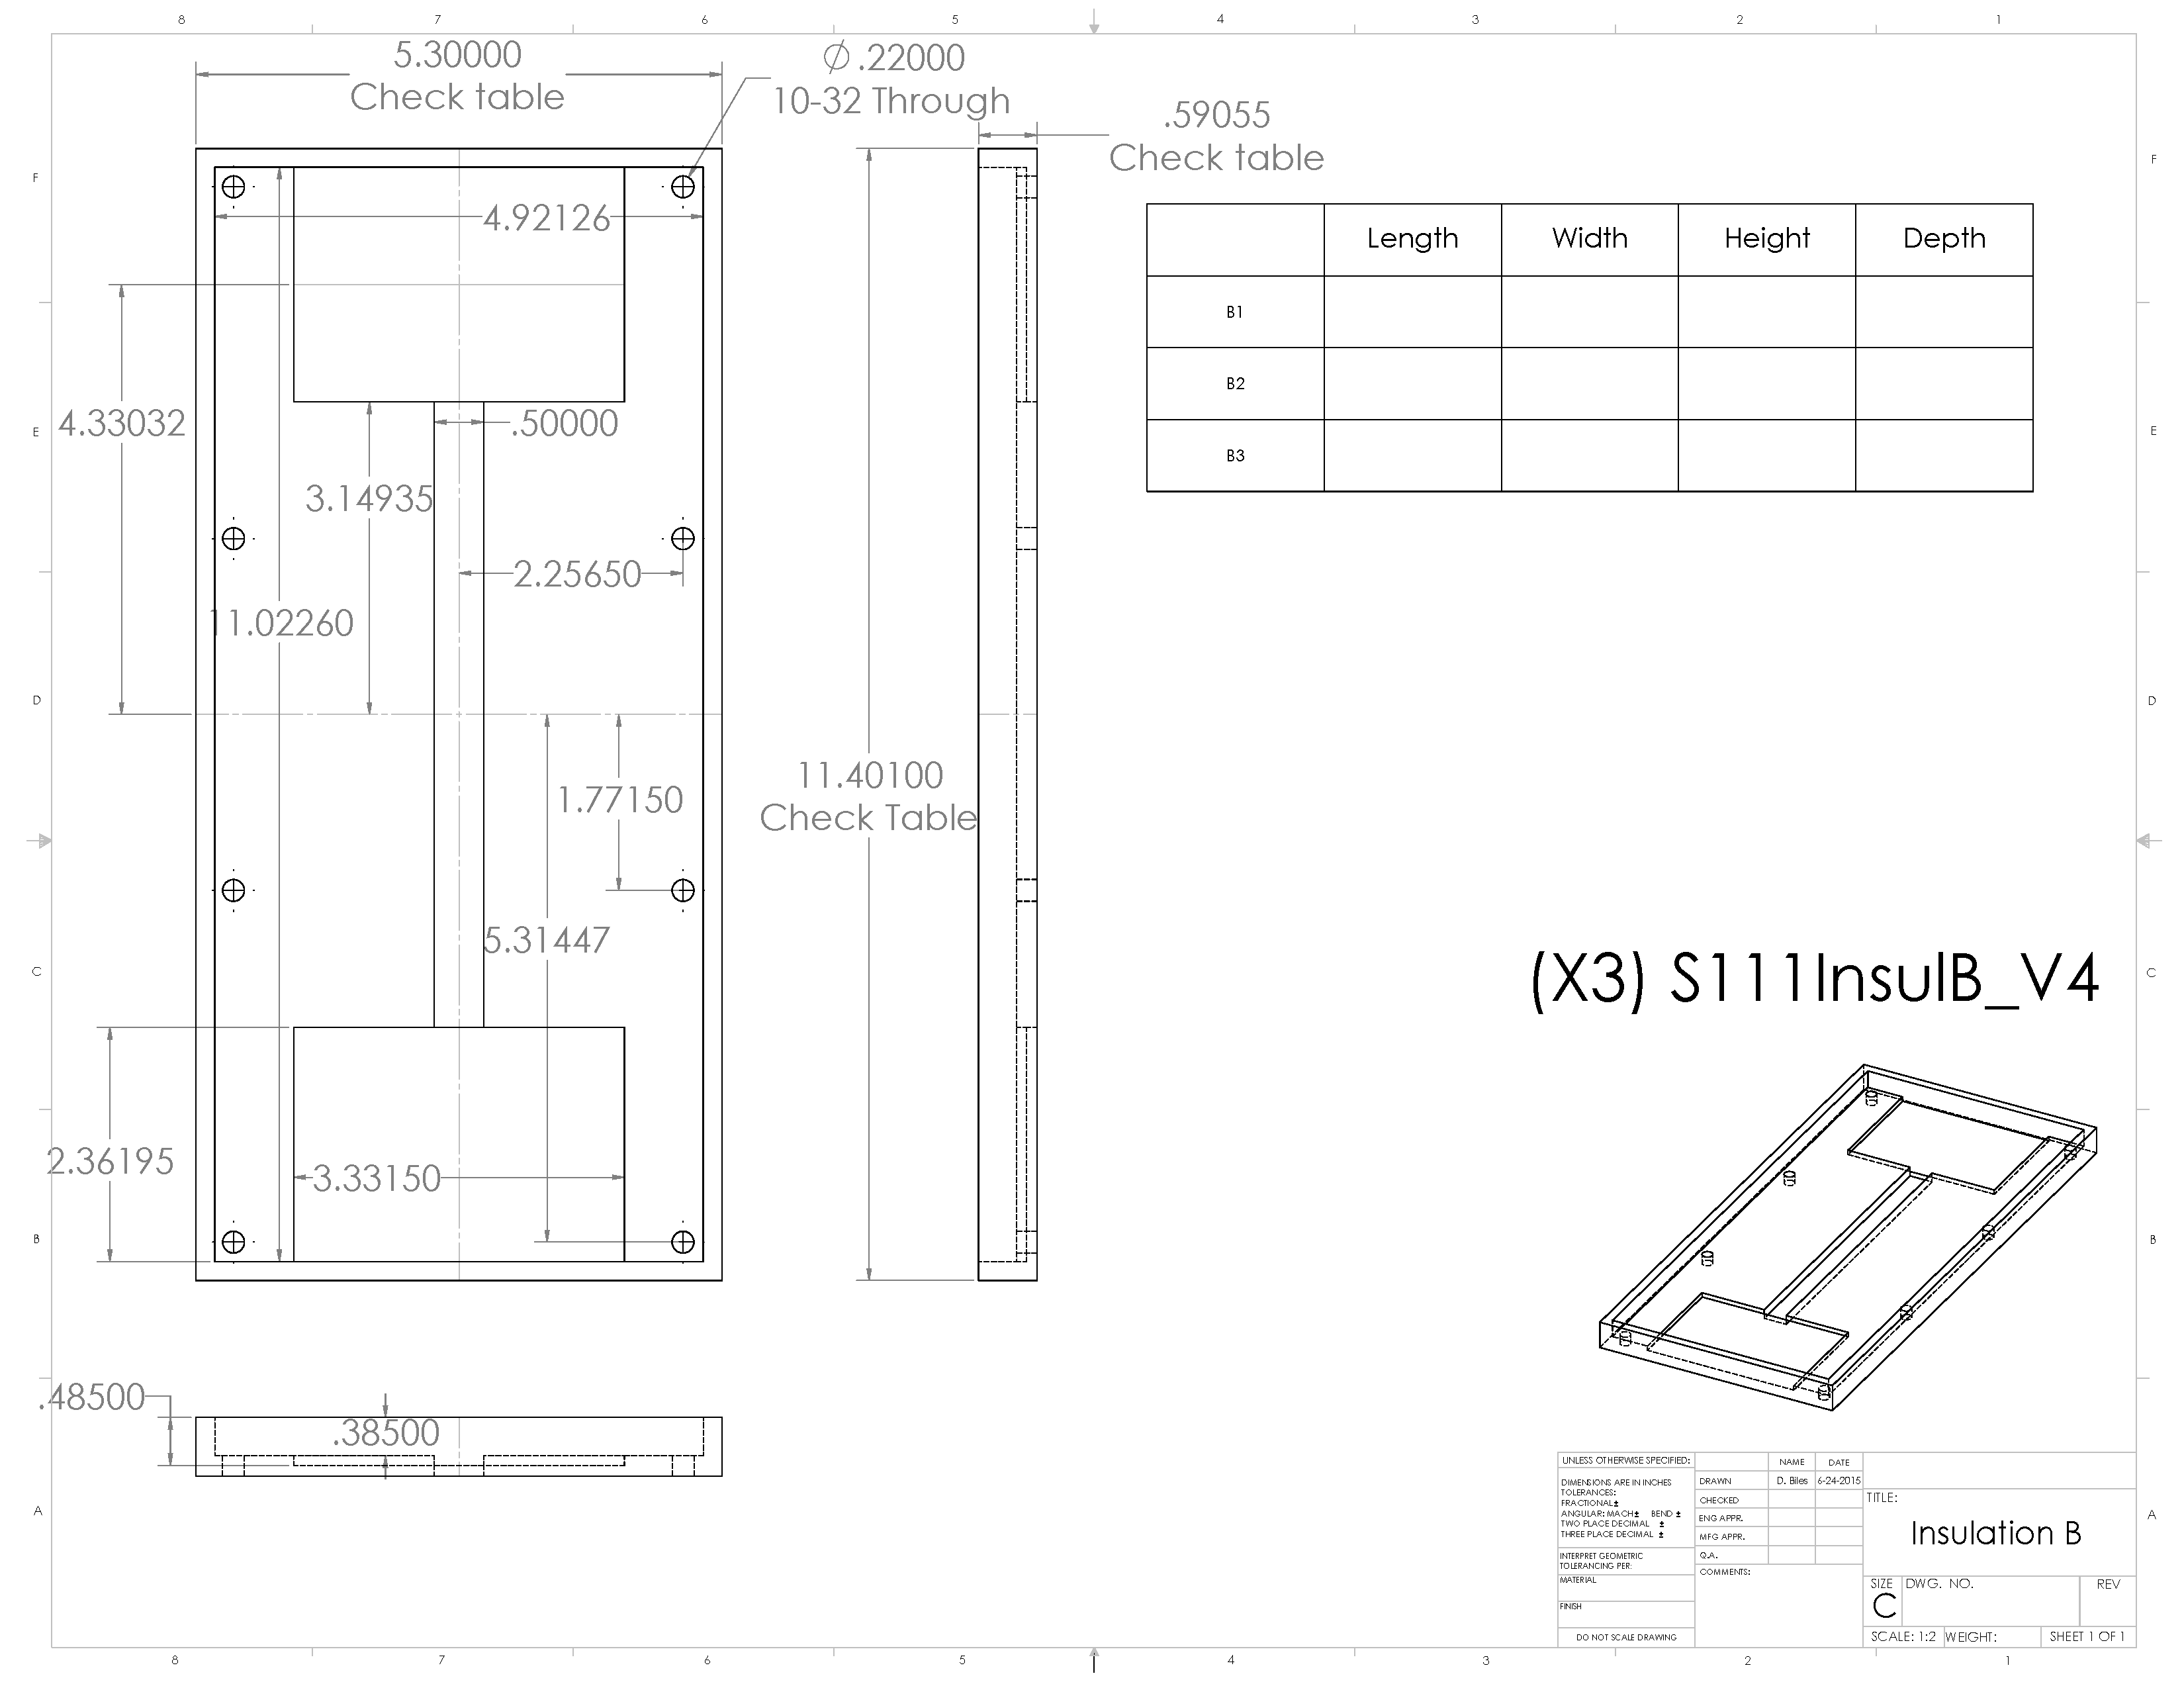
\includegraphics[scale=.2]{facility/drawings/Insulation_B.PDF}
\caption{\footnotesize {\bf XX} } 
\end{figure}

\begin{figure}[h!]
\centering
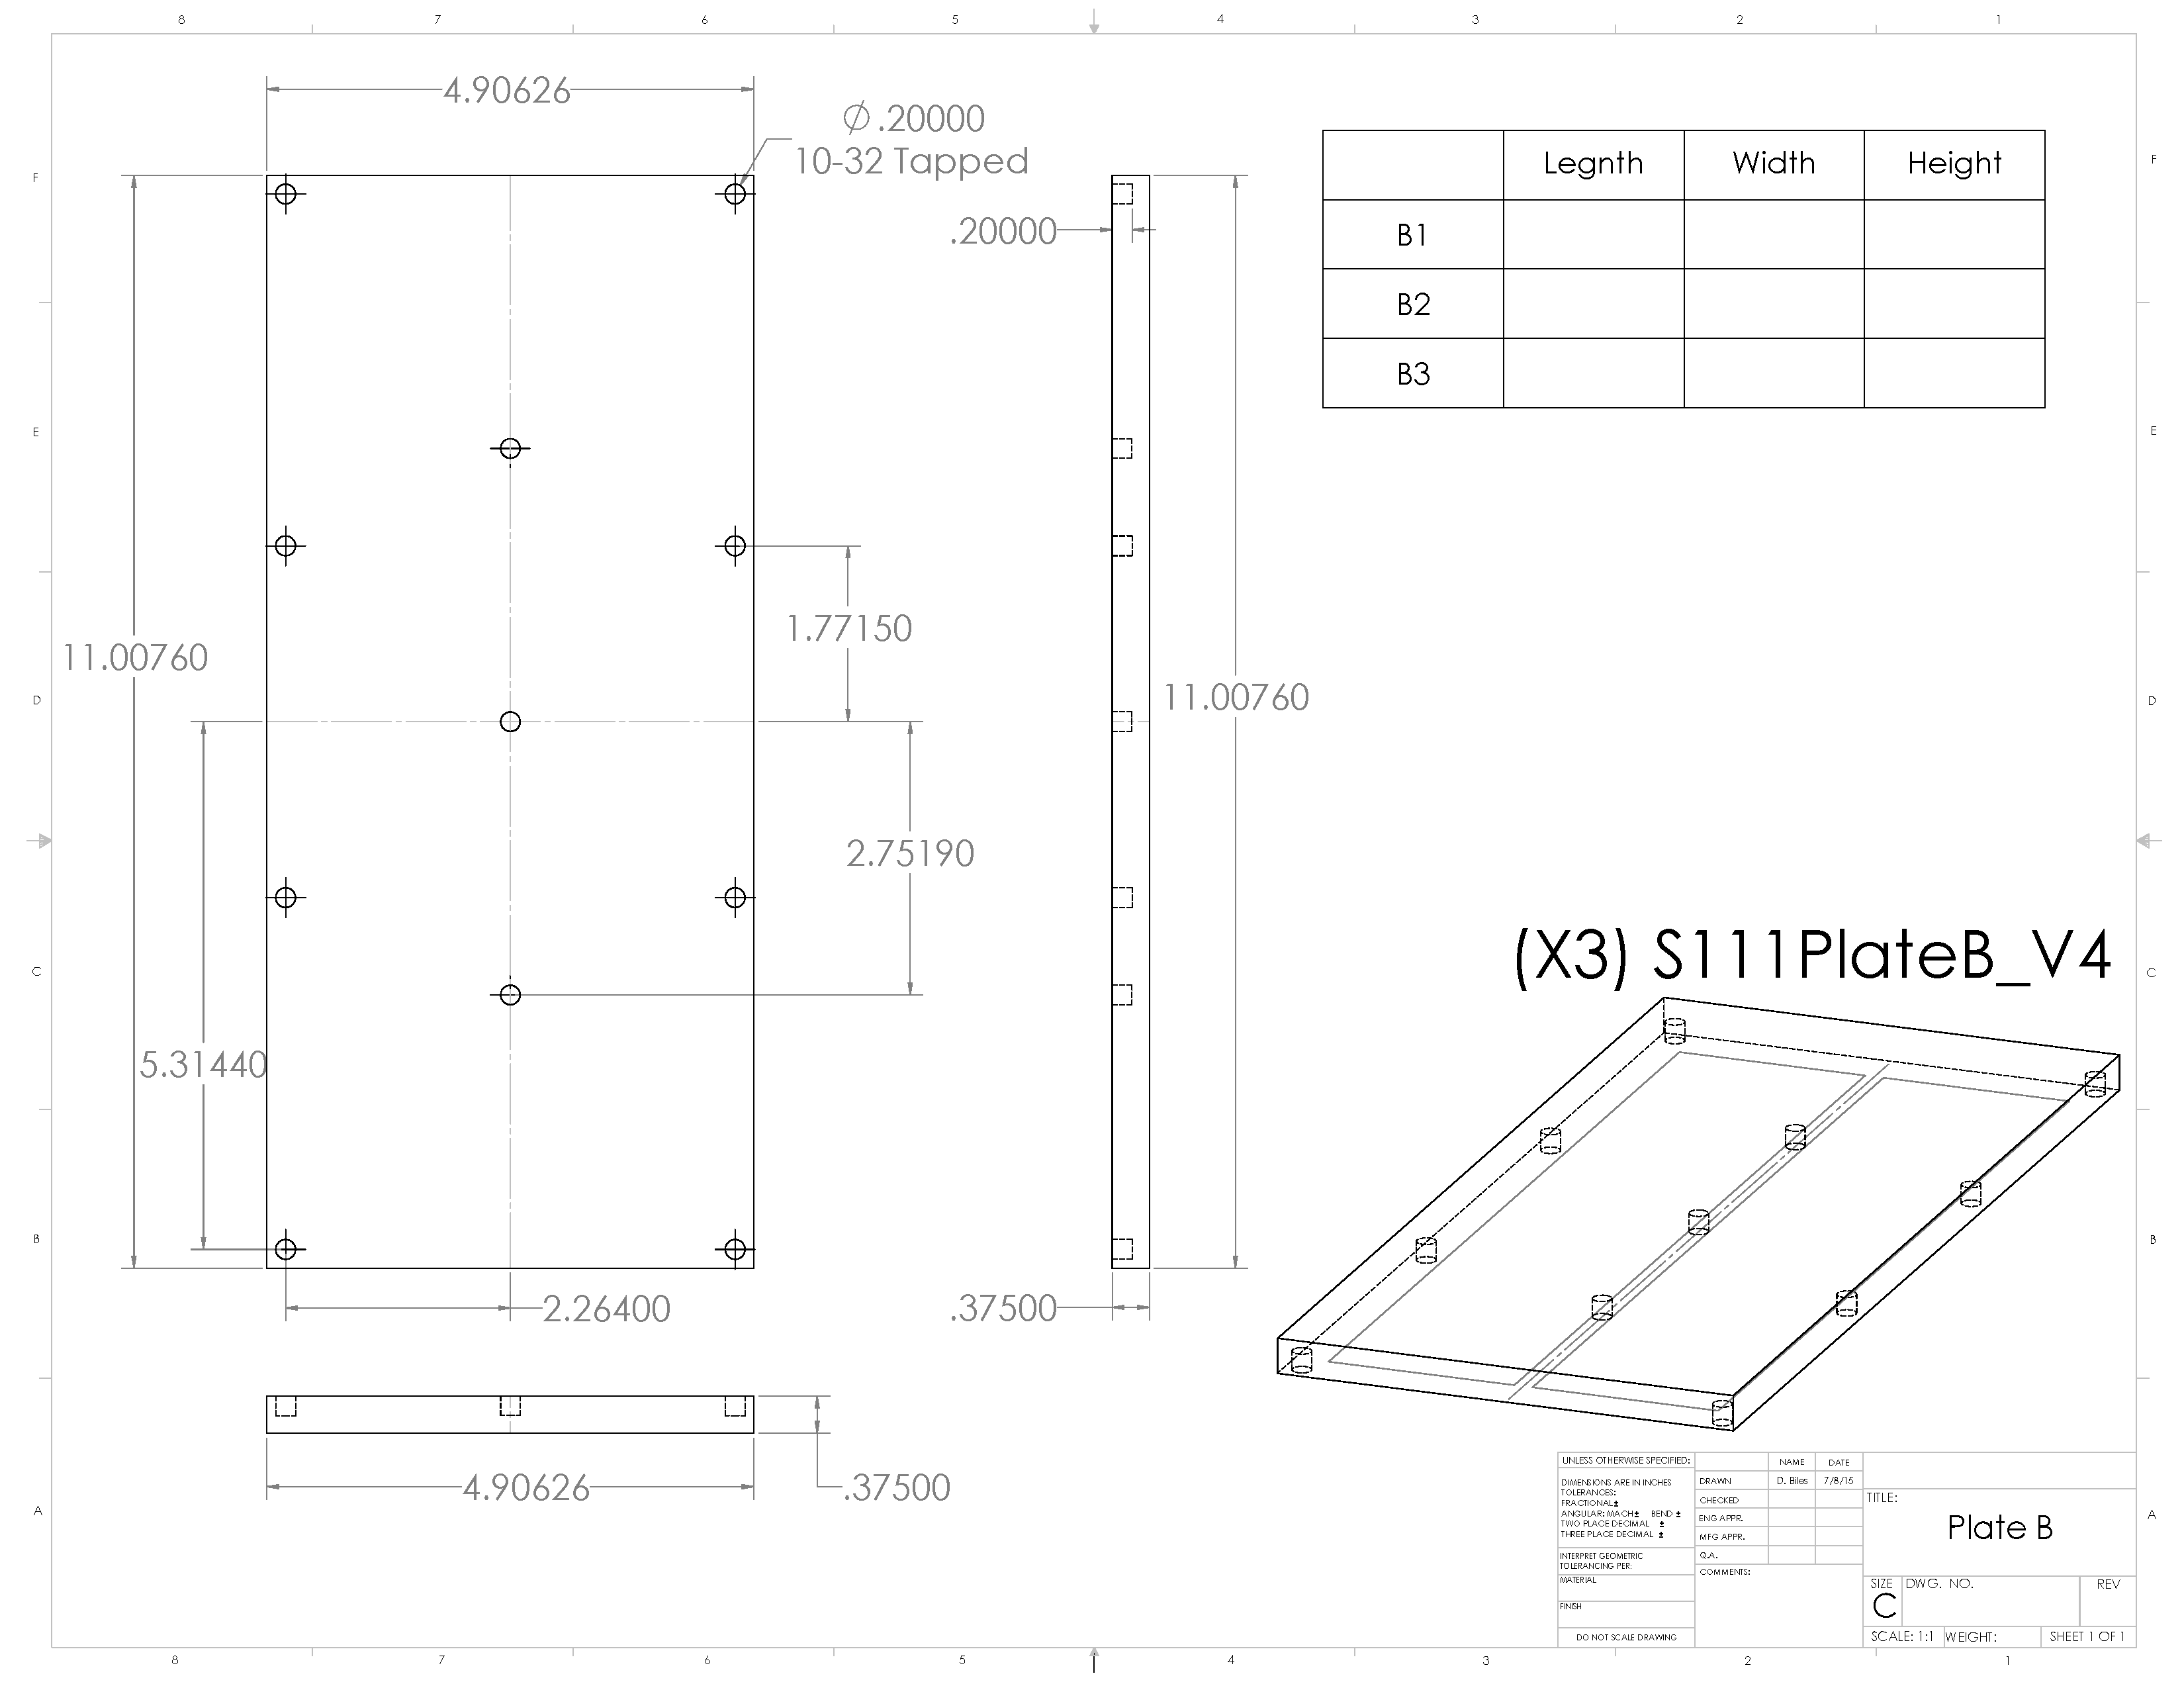
\includegraphics[scale=.2]{facility/drawings/Plate_B.PDF}
\caption{\footnotesize {\bf XX} } 
\end{figure}

\begin{figure}[h!]
  \begin{center}
  {\subfigcapskip = 5pt \subfigcapmargin = -12pt \subfigure[]{\label{fig:edge-a}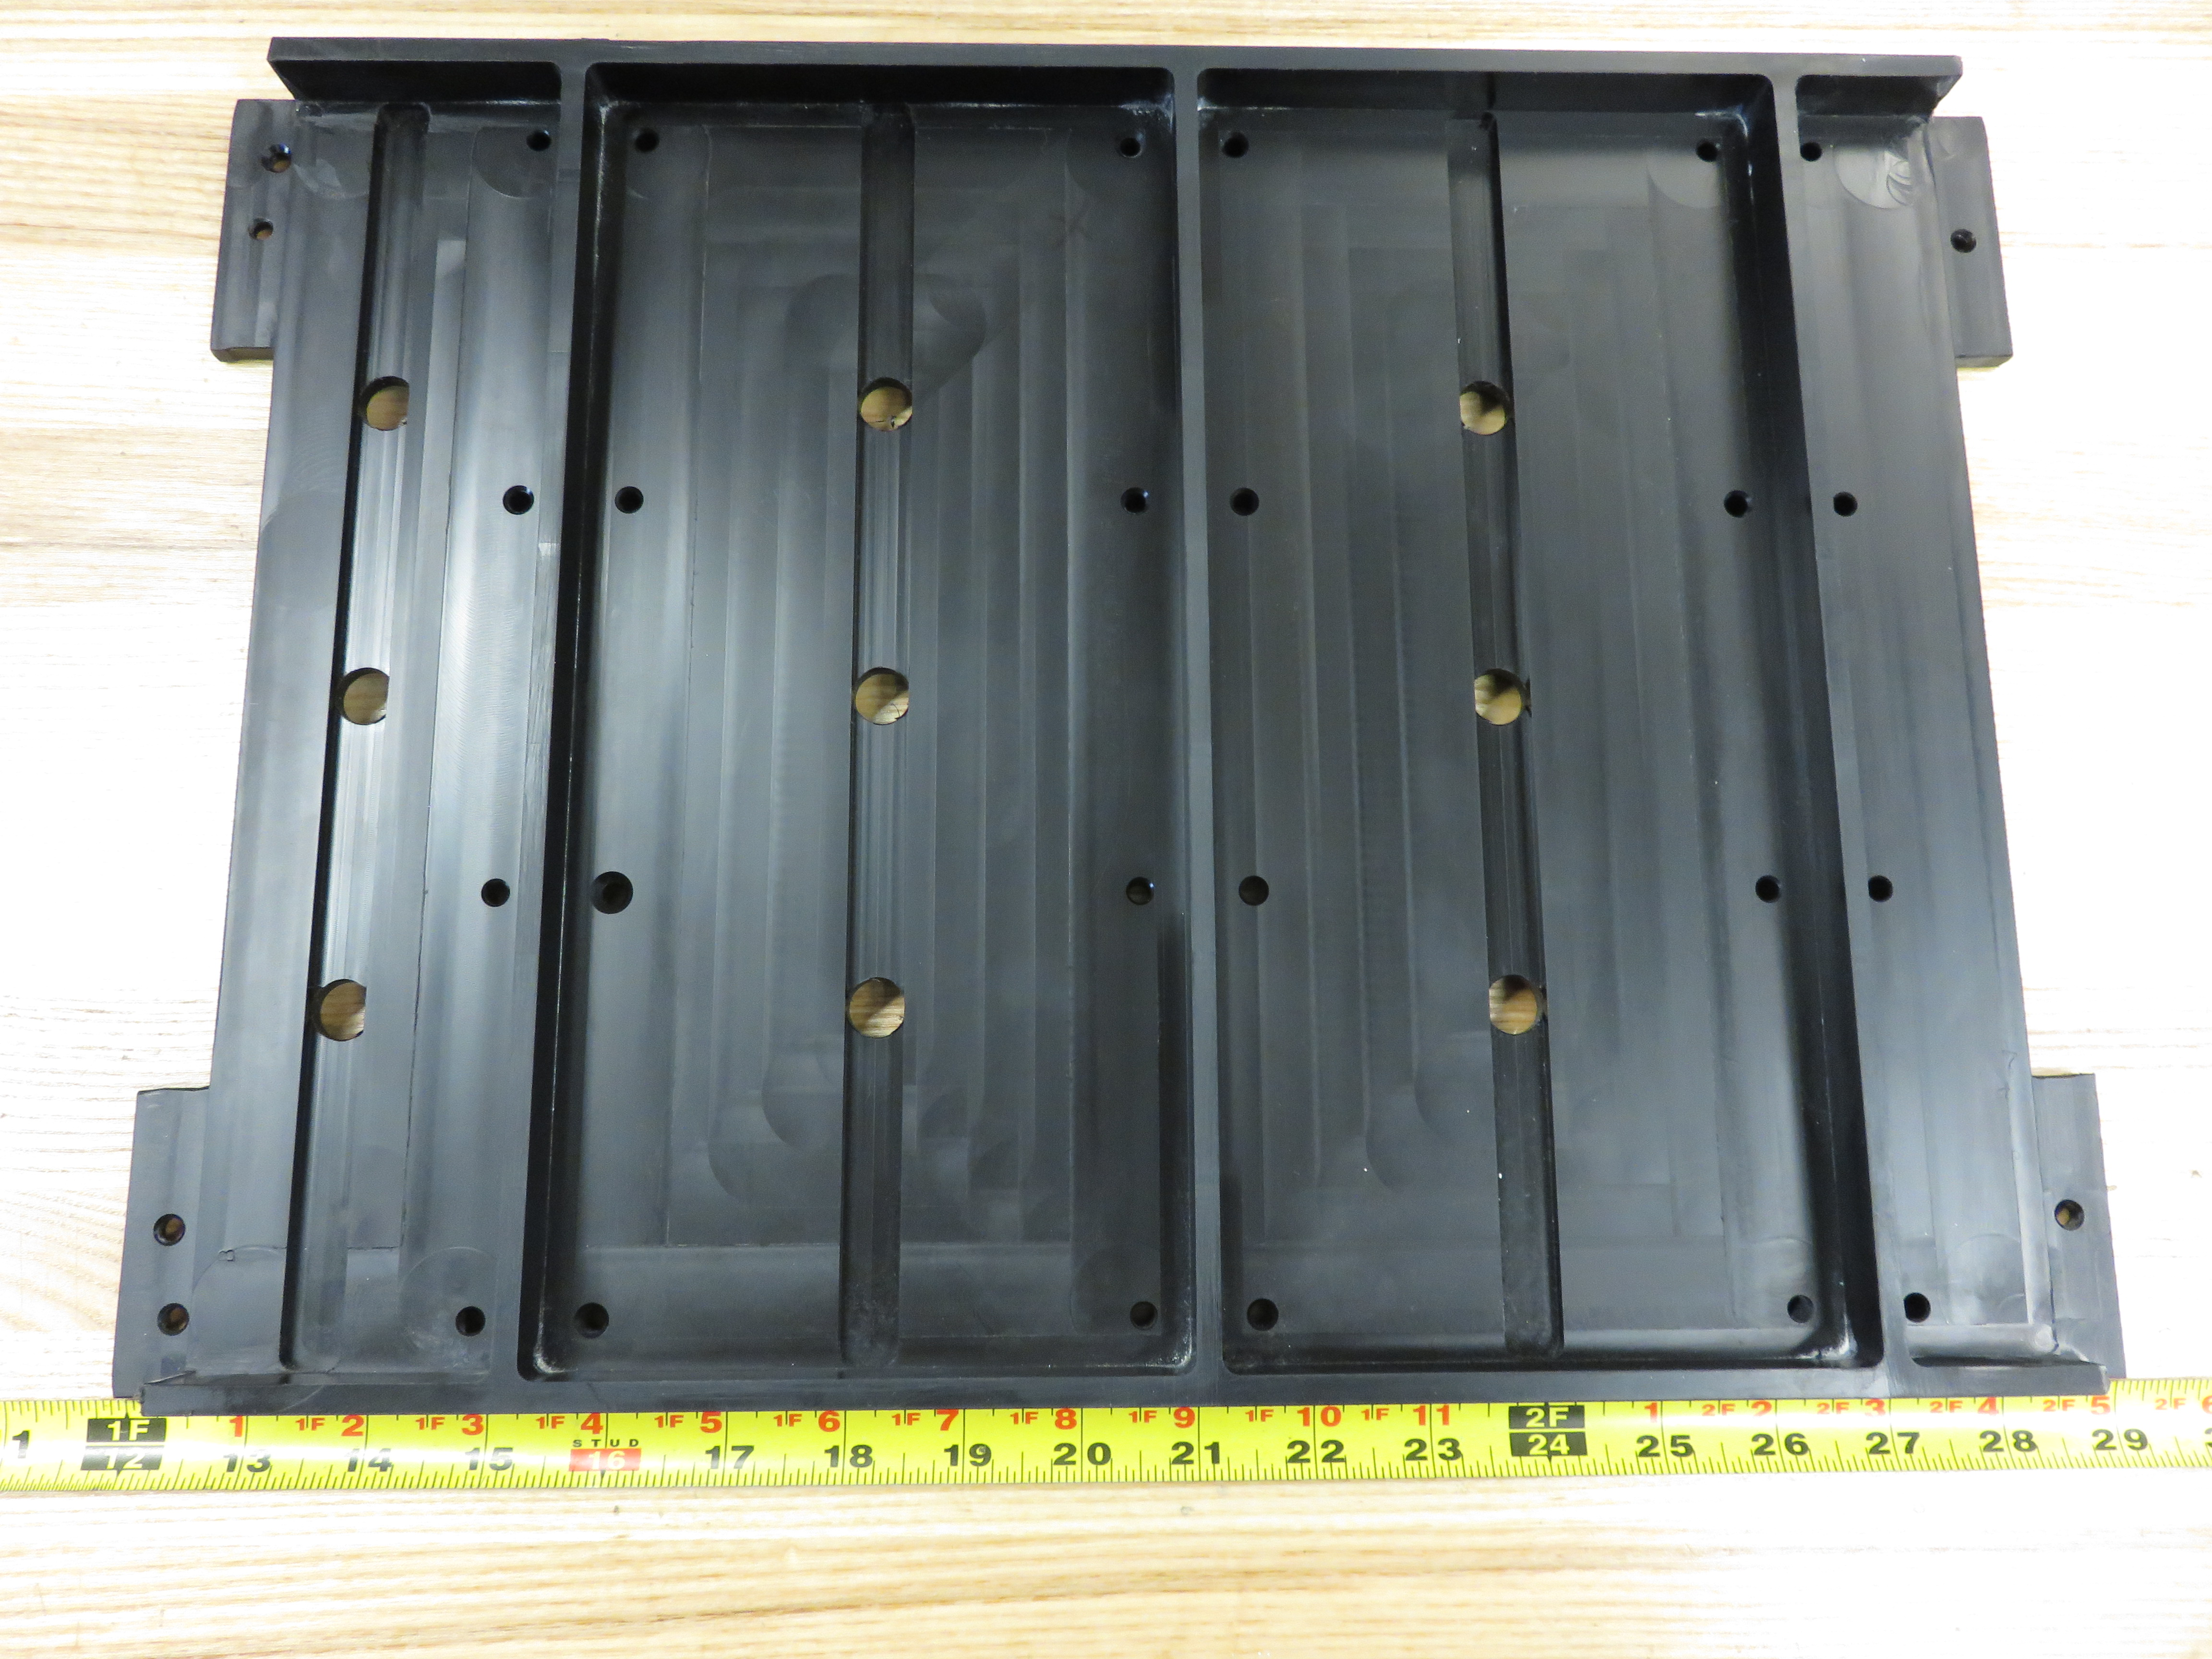
\includegraphics[scale=0.2]{facility/MachinedParts/B_meas_v2.JPG}}}
   {\subfigcapskip = 5pt \subfigcapmargin = -12pt  \subfigure[]{\label{fig:edge-b}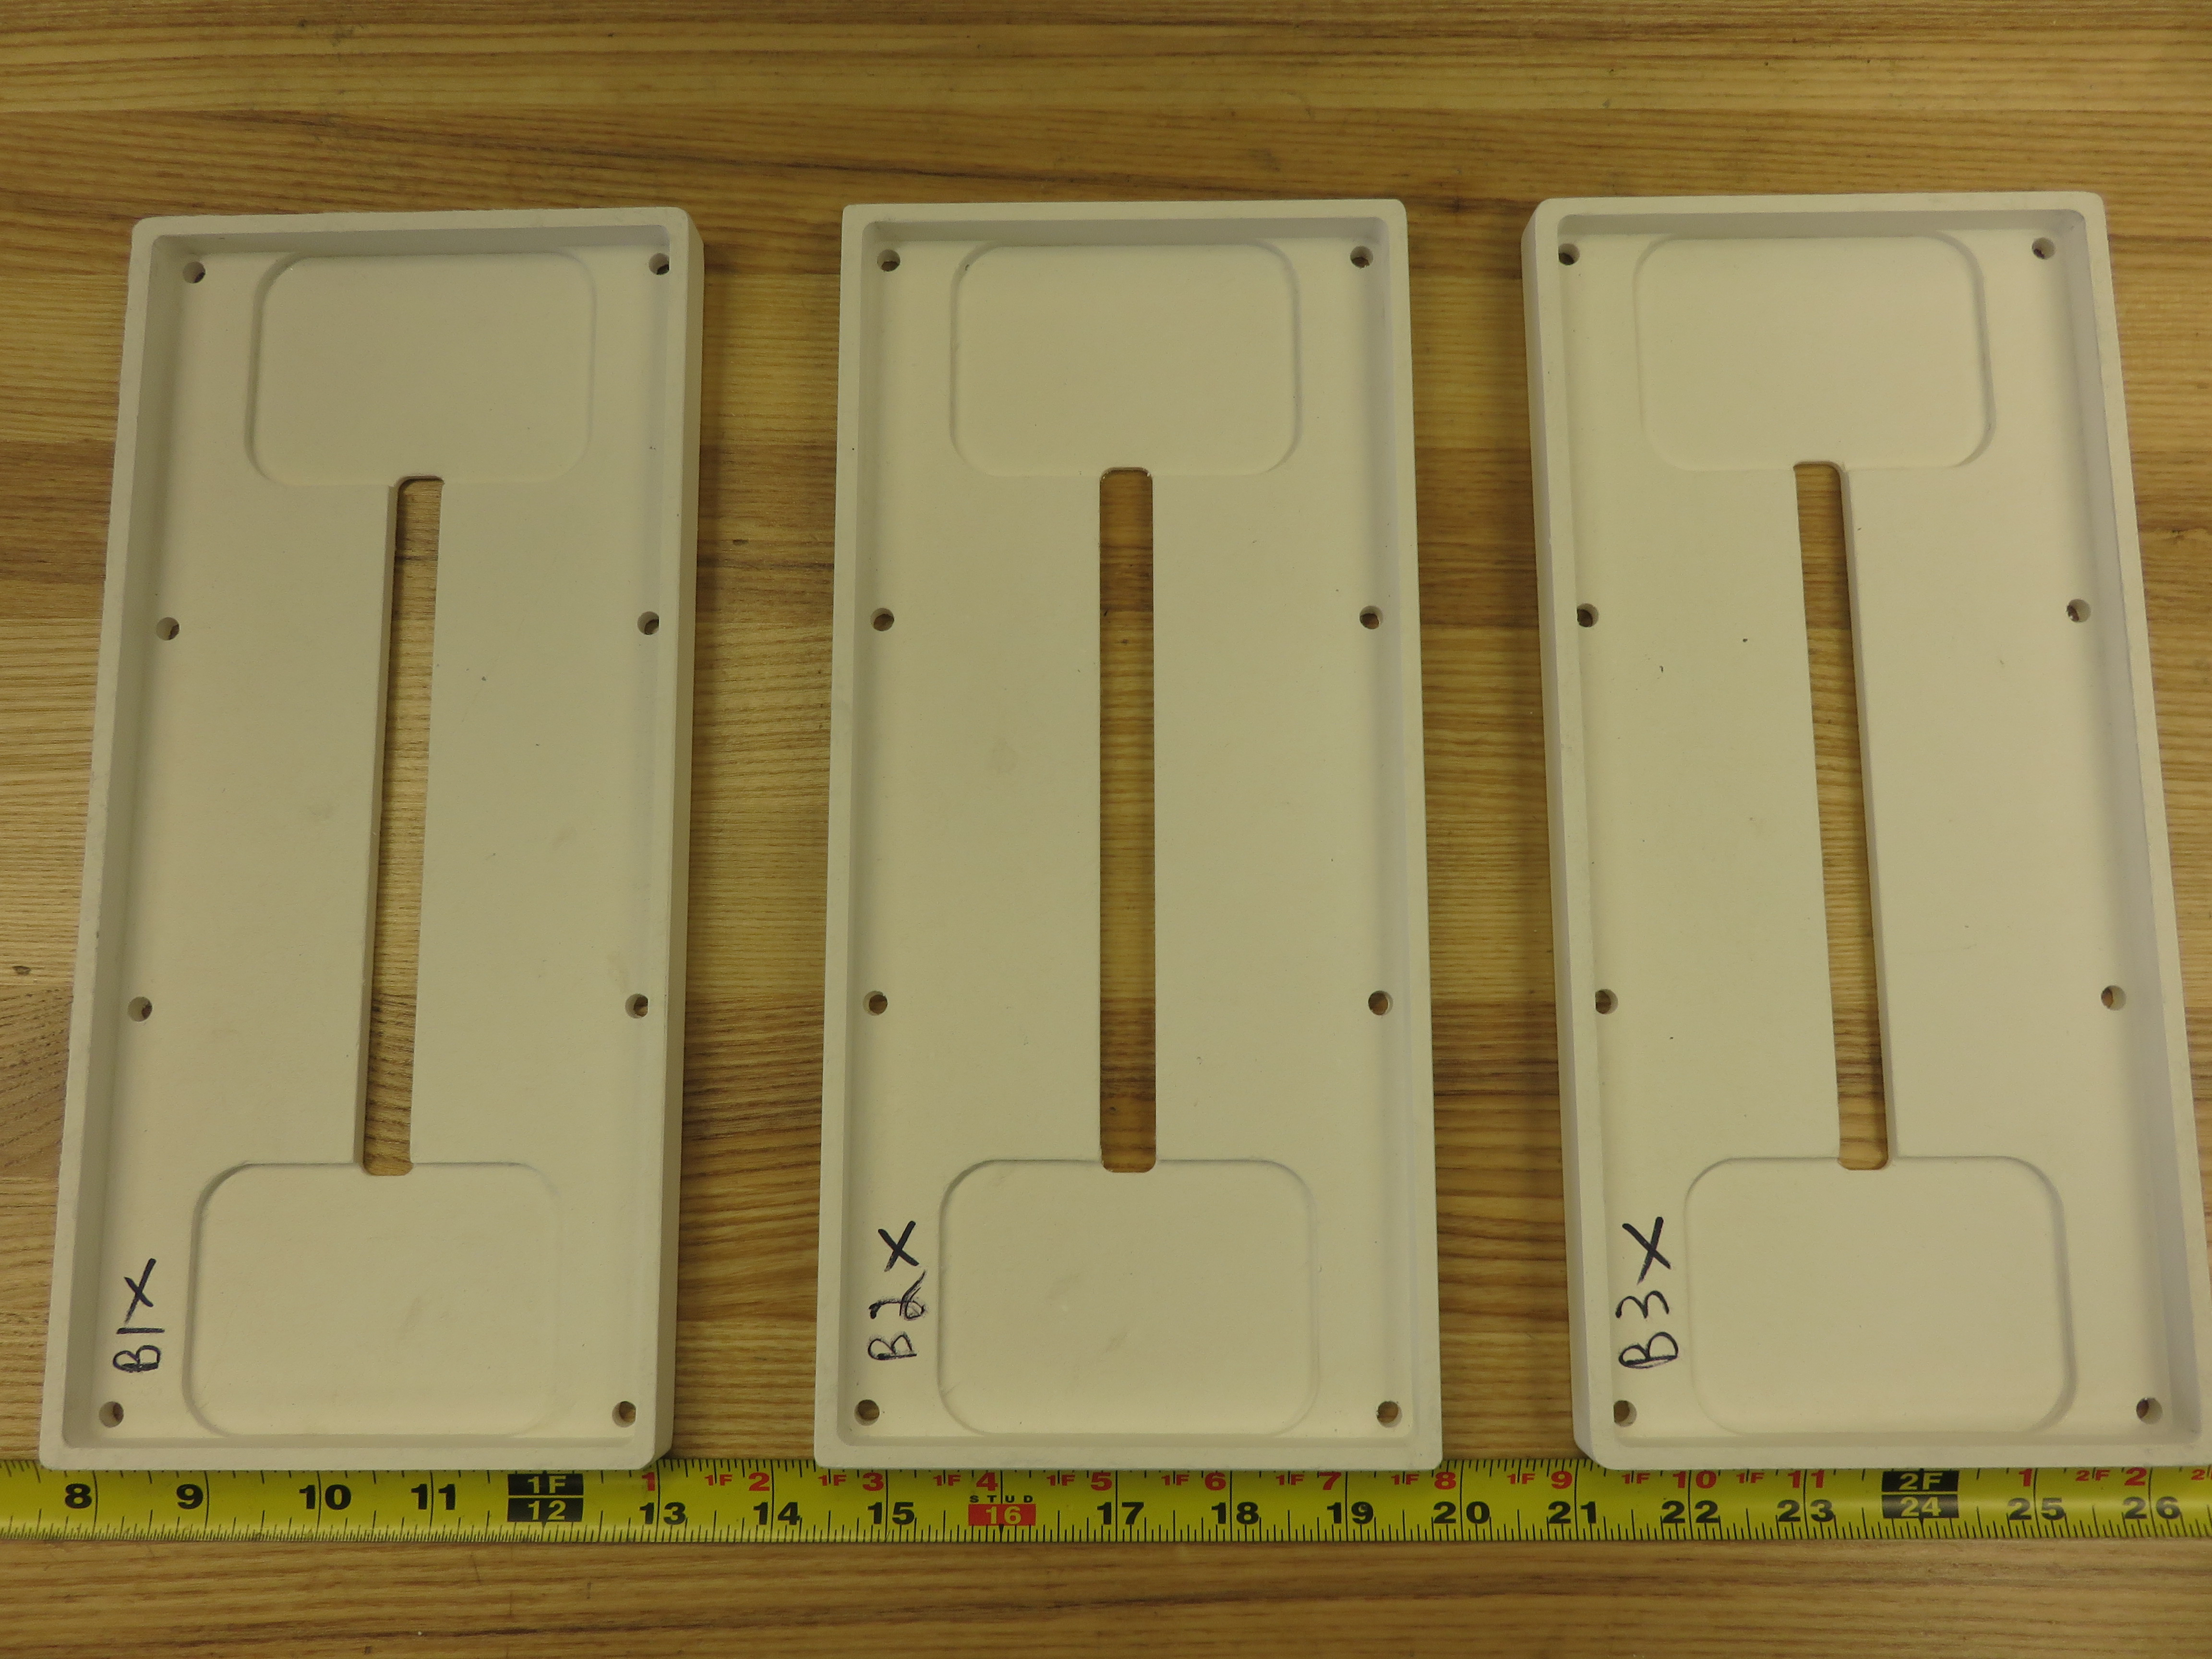
\includegraphics[scale=0.2]{facility/MachinedParts/B_insul_v2.JPG}}}
  \end{center}
\caption{(a) insulation (b) frame. } 
\end{figure}


%%%%%%%%%%%%%%%%%%%%%%%%%%%%%%%%%%%%%%%%%%%%%%%%%%%%%%
\clearpage
\subsection{Components C}
Input text description?\\

%components C
\begin{figure}[h!]
\centering
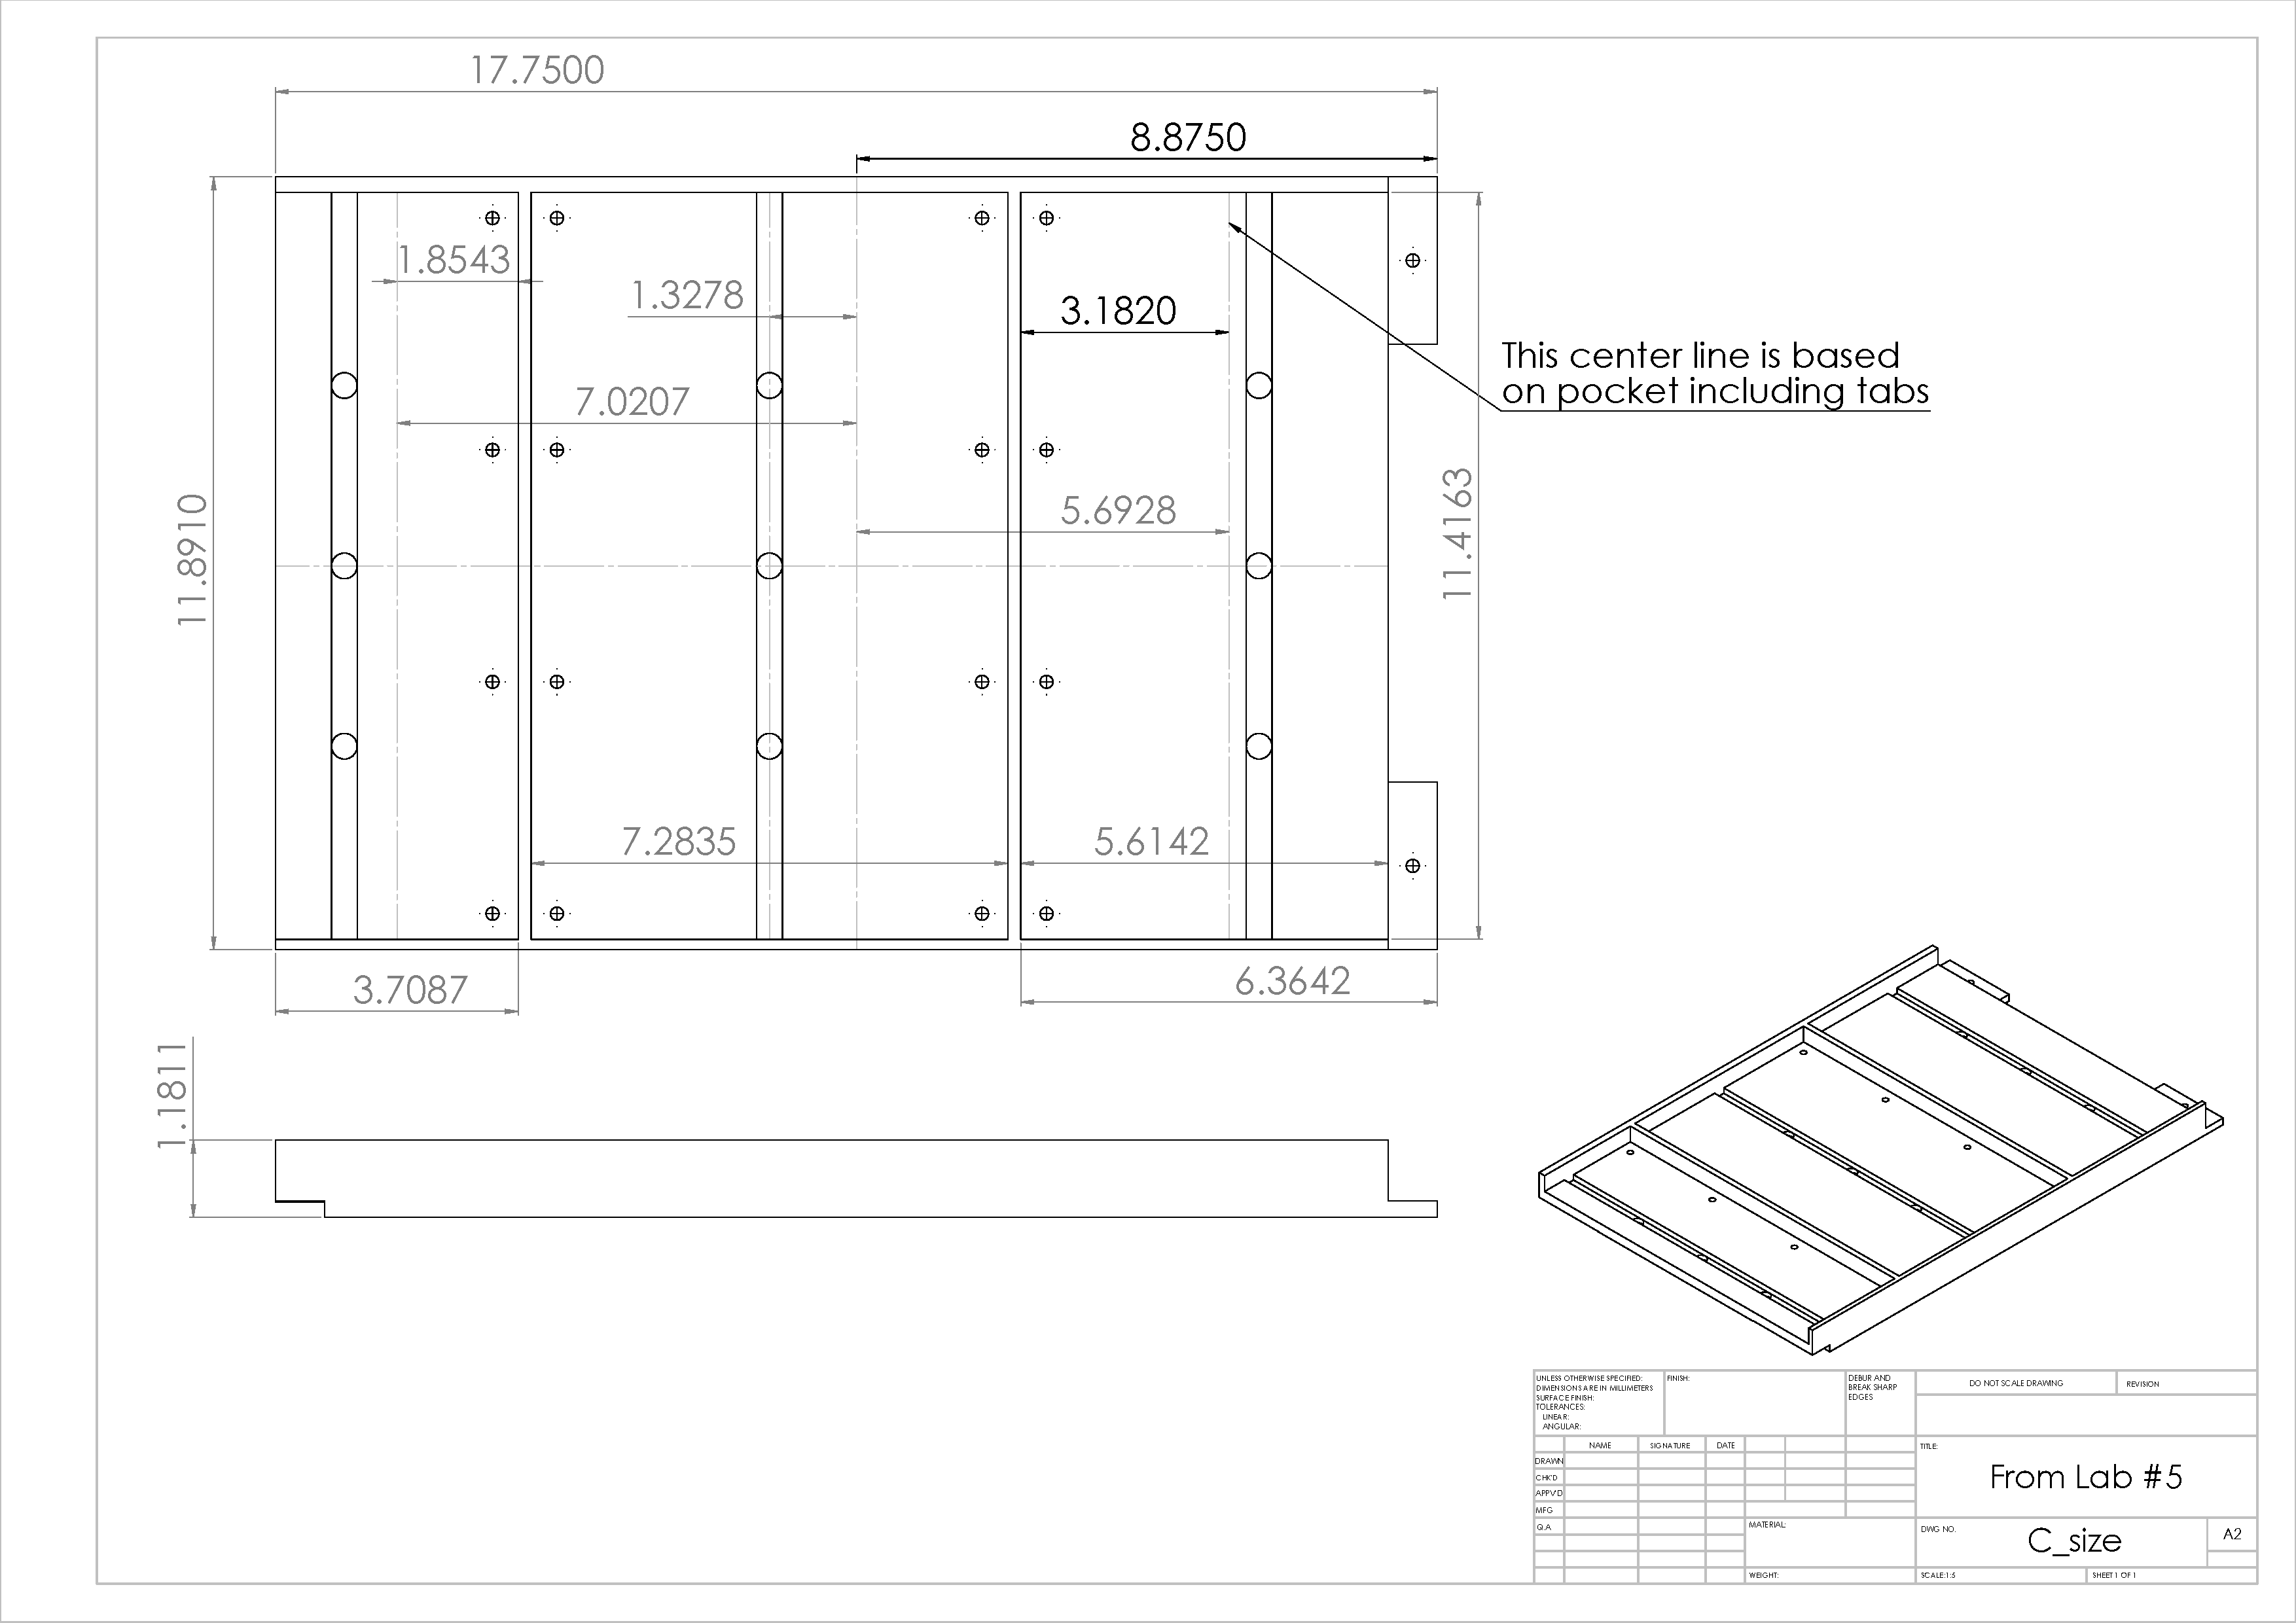
\includegraphics[scale=.2]{facility/drawings/C_size.PDF}
\caption{\footnotesize {\bf XX} } 
\end{figure}

\begin{figure}[h!]
\centering
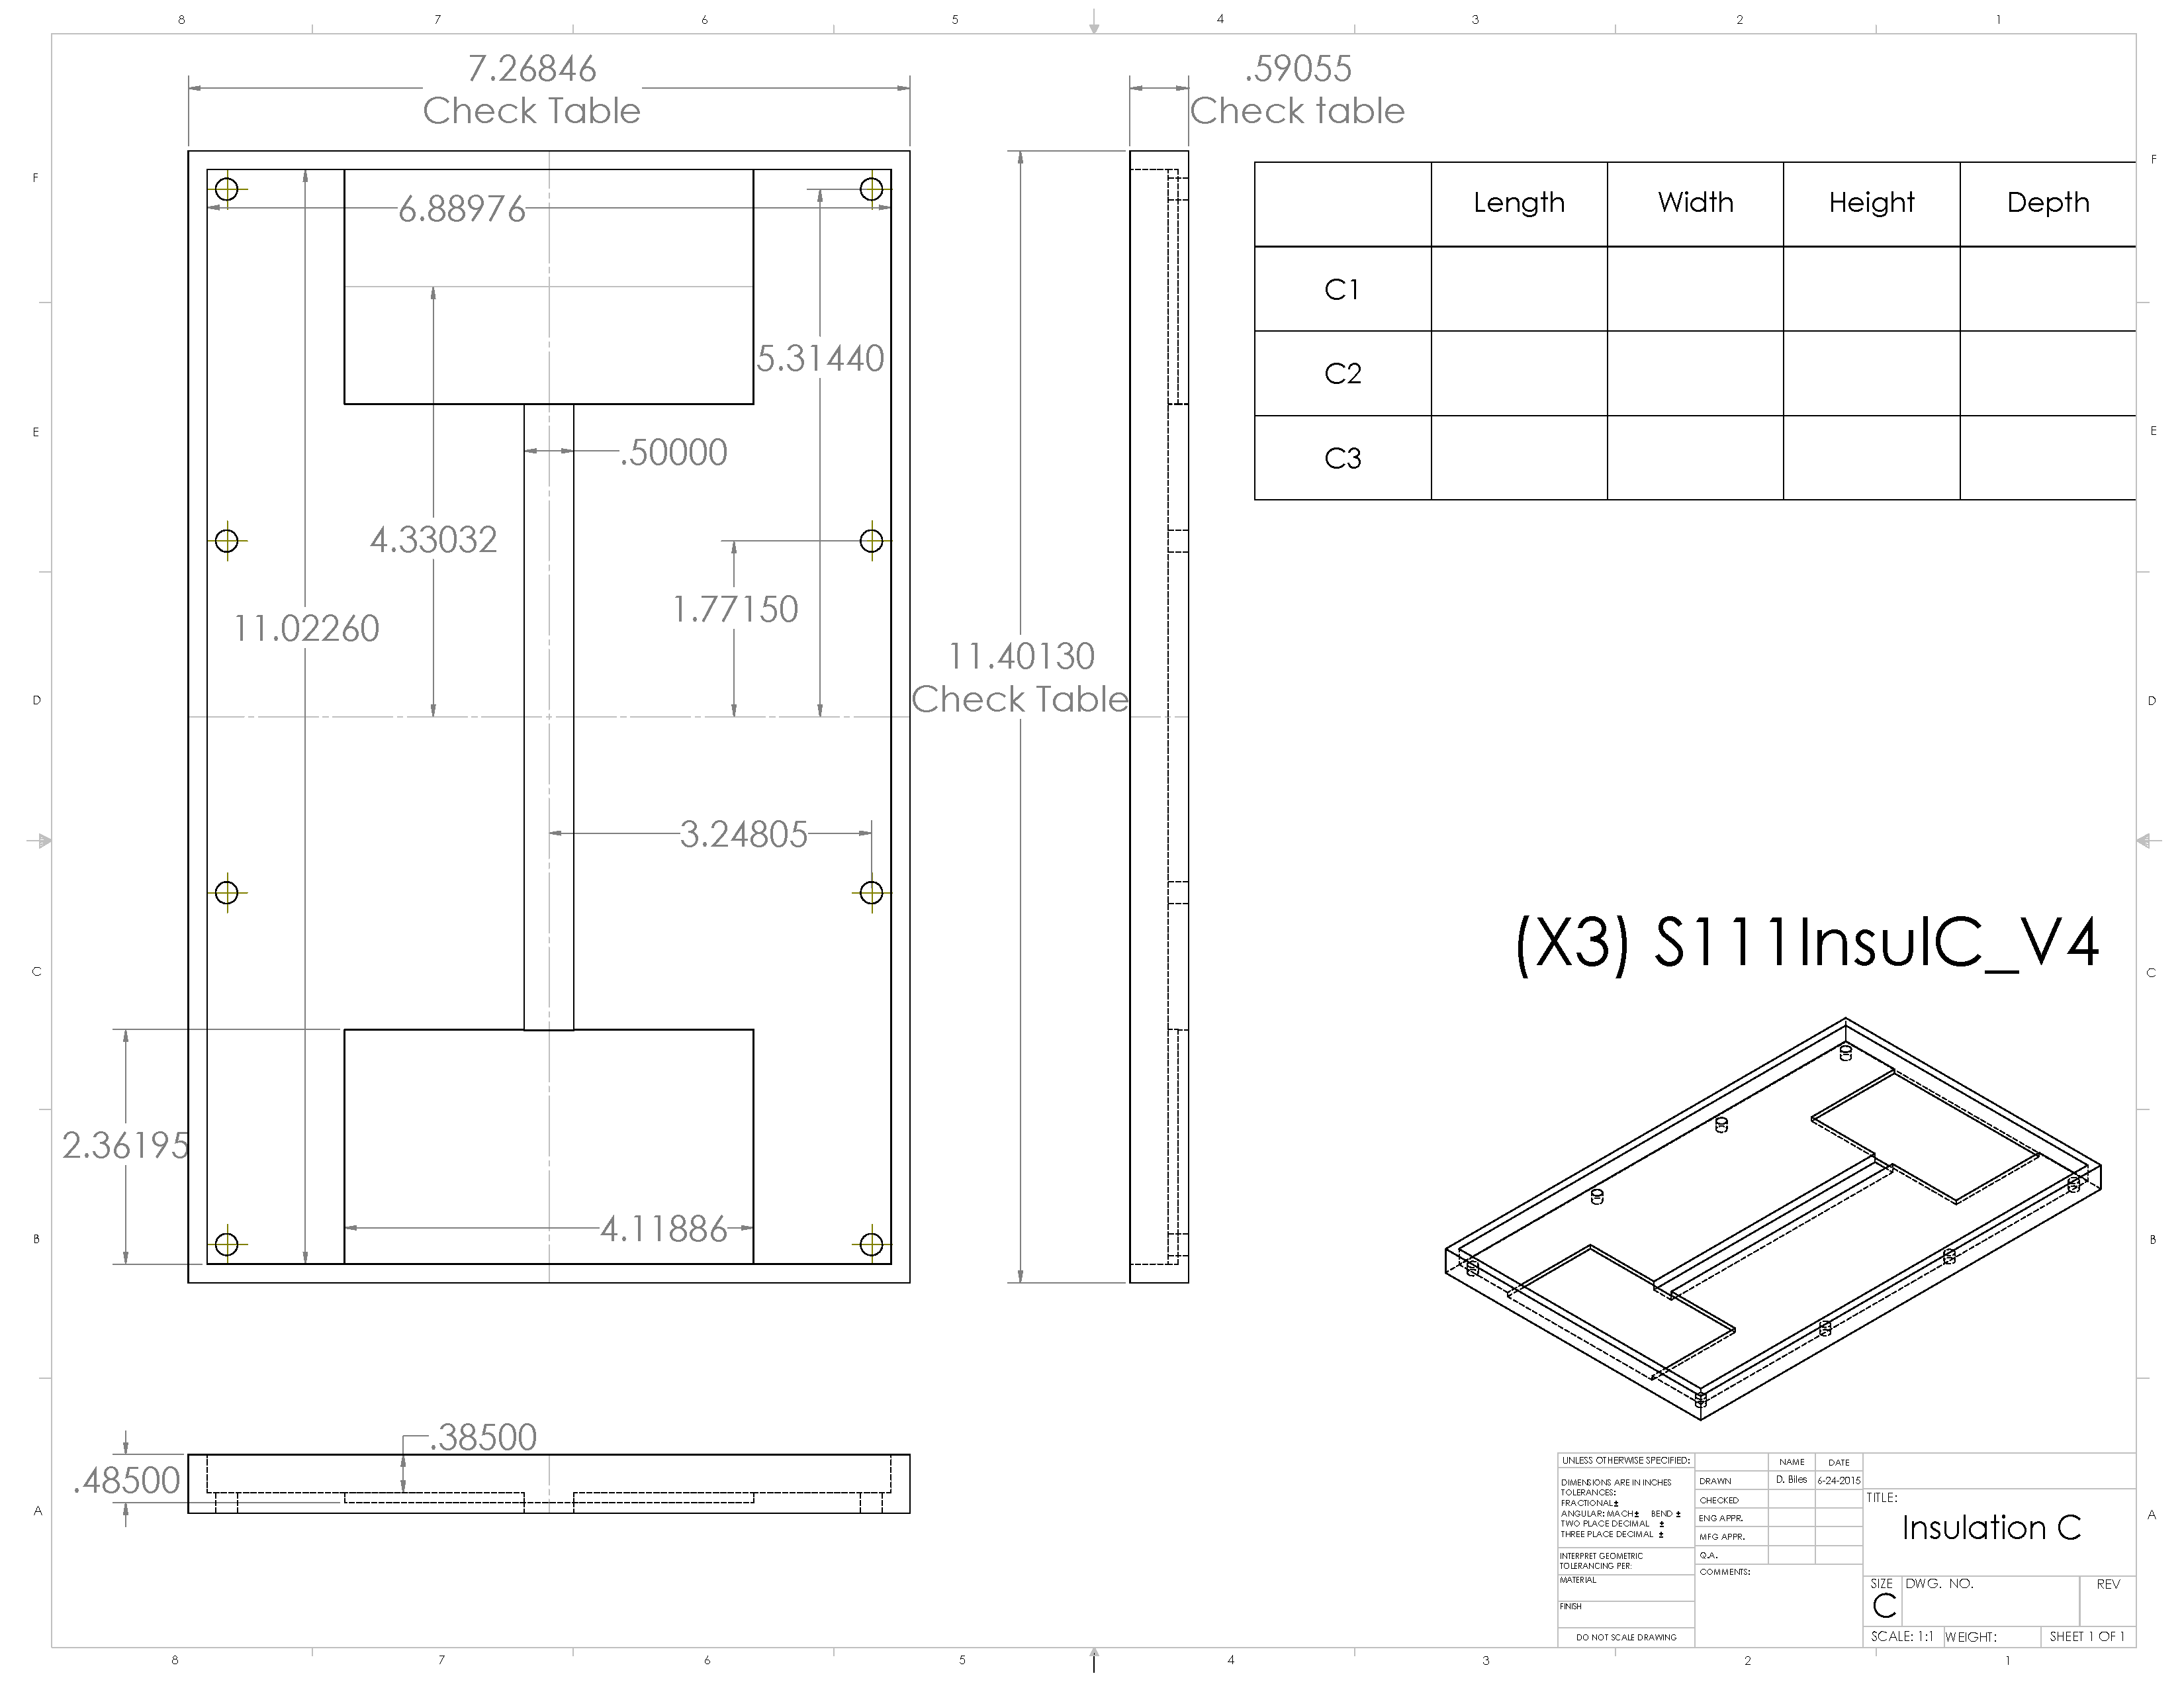
\includegraphics[scale=.2]{facility/drawings/Insulation_C.PDF}
\caption{\footnotesize {\bf XX} } 
\end{figure}

\begin{figure}[h!]
\centering
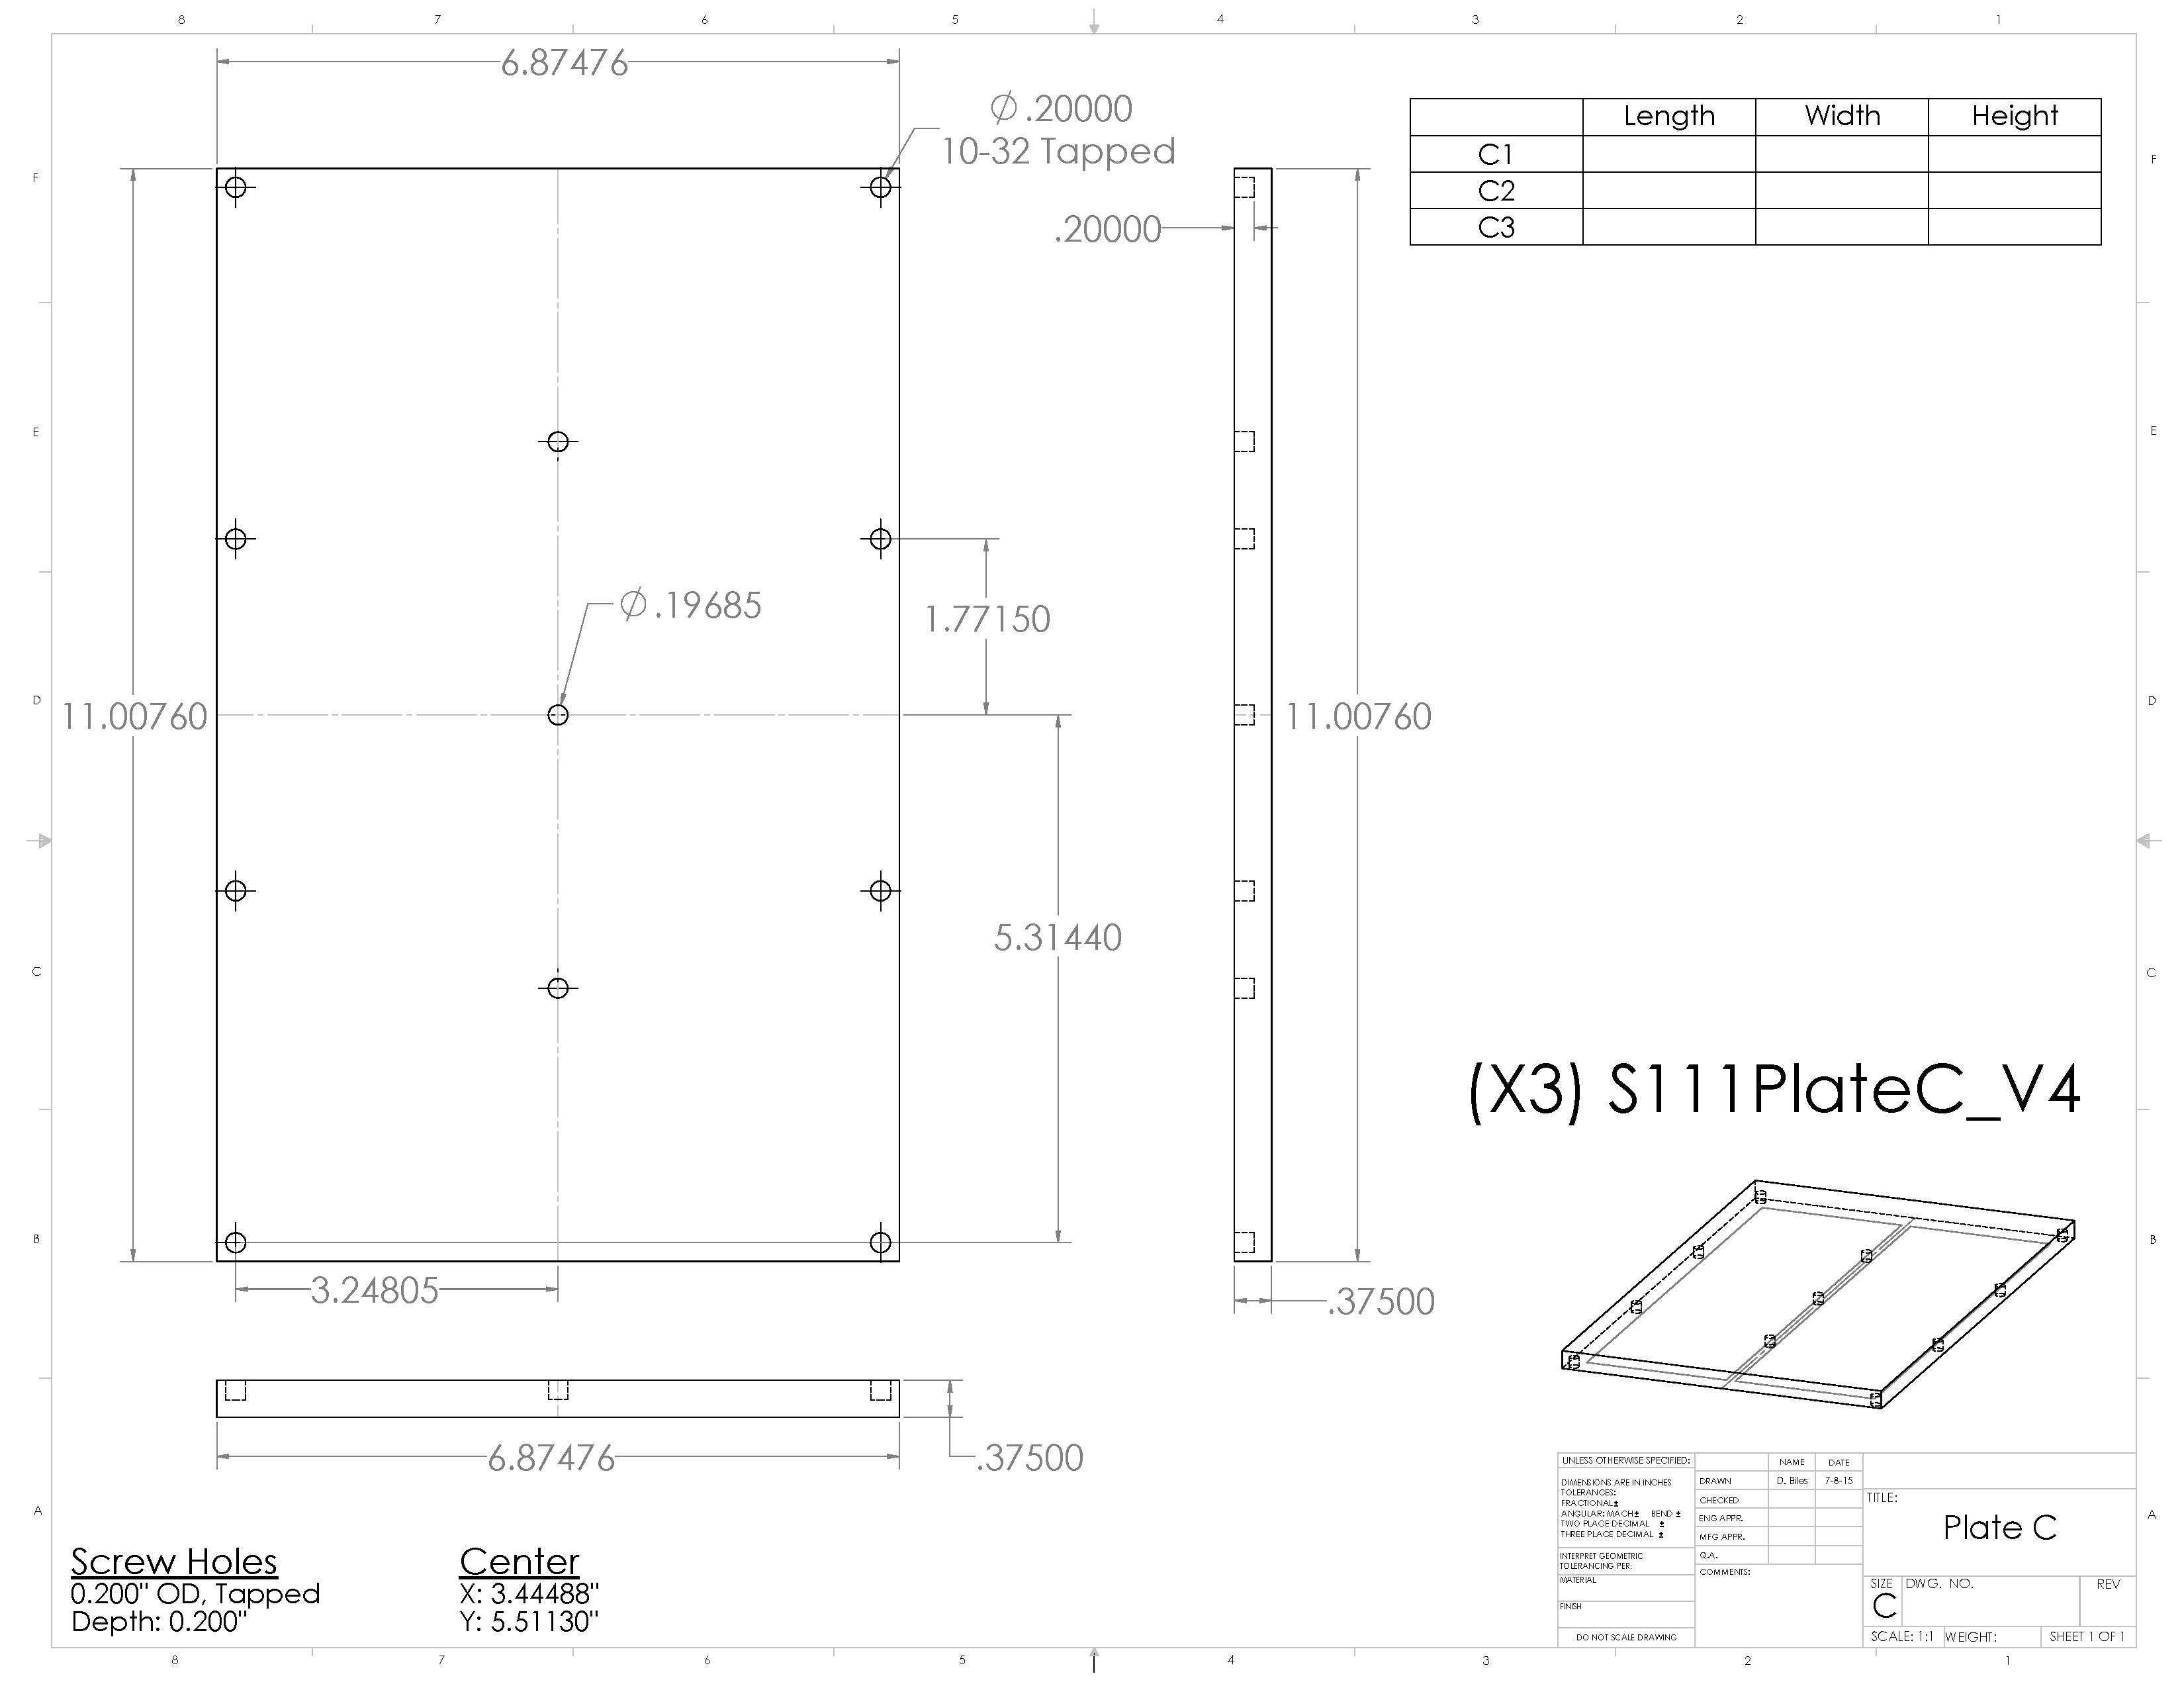
\includegraphics[scale=.2]{facility/drawings/Plate_C.PDF}
\caption{\footnotesize {\bf XX} } 
\end{figure}

\begin{figure}[h!]
  \begin{center}
  {\subfigcapskip = 5pt \subfigcapmargin = -12pt \subfigure[]{\label{fig:edge-a}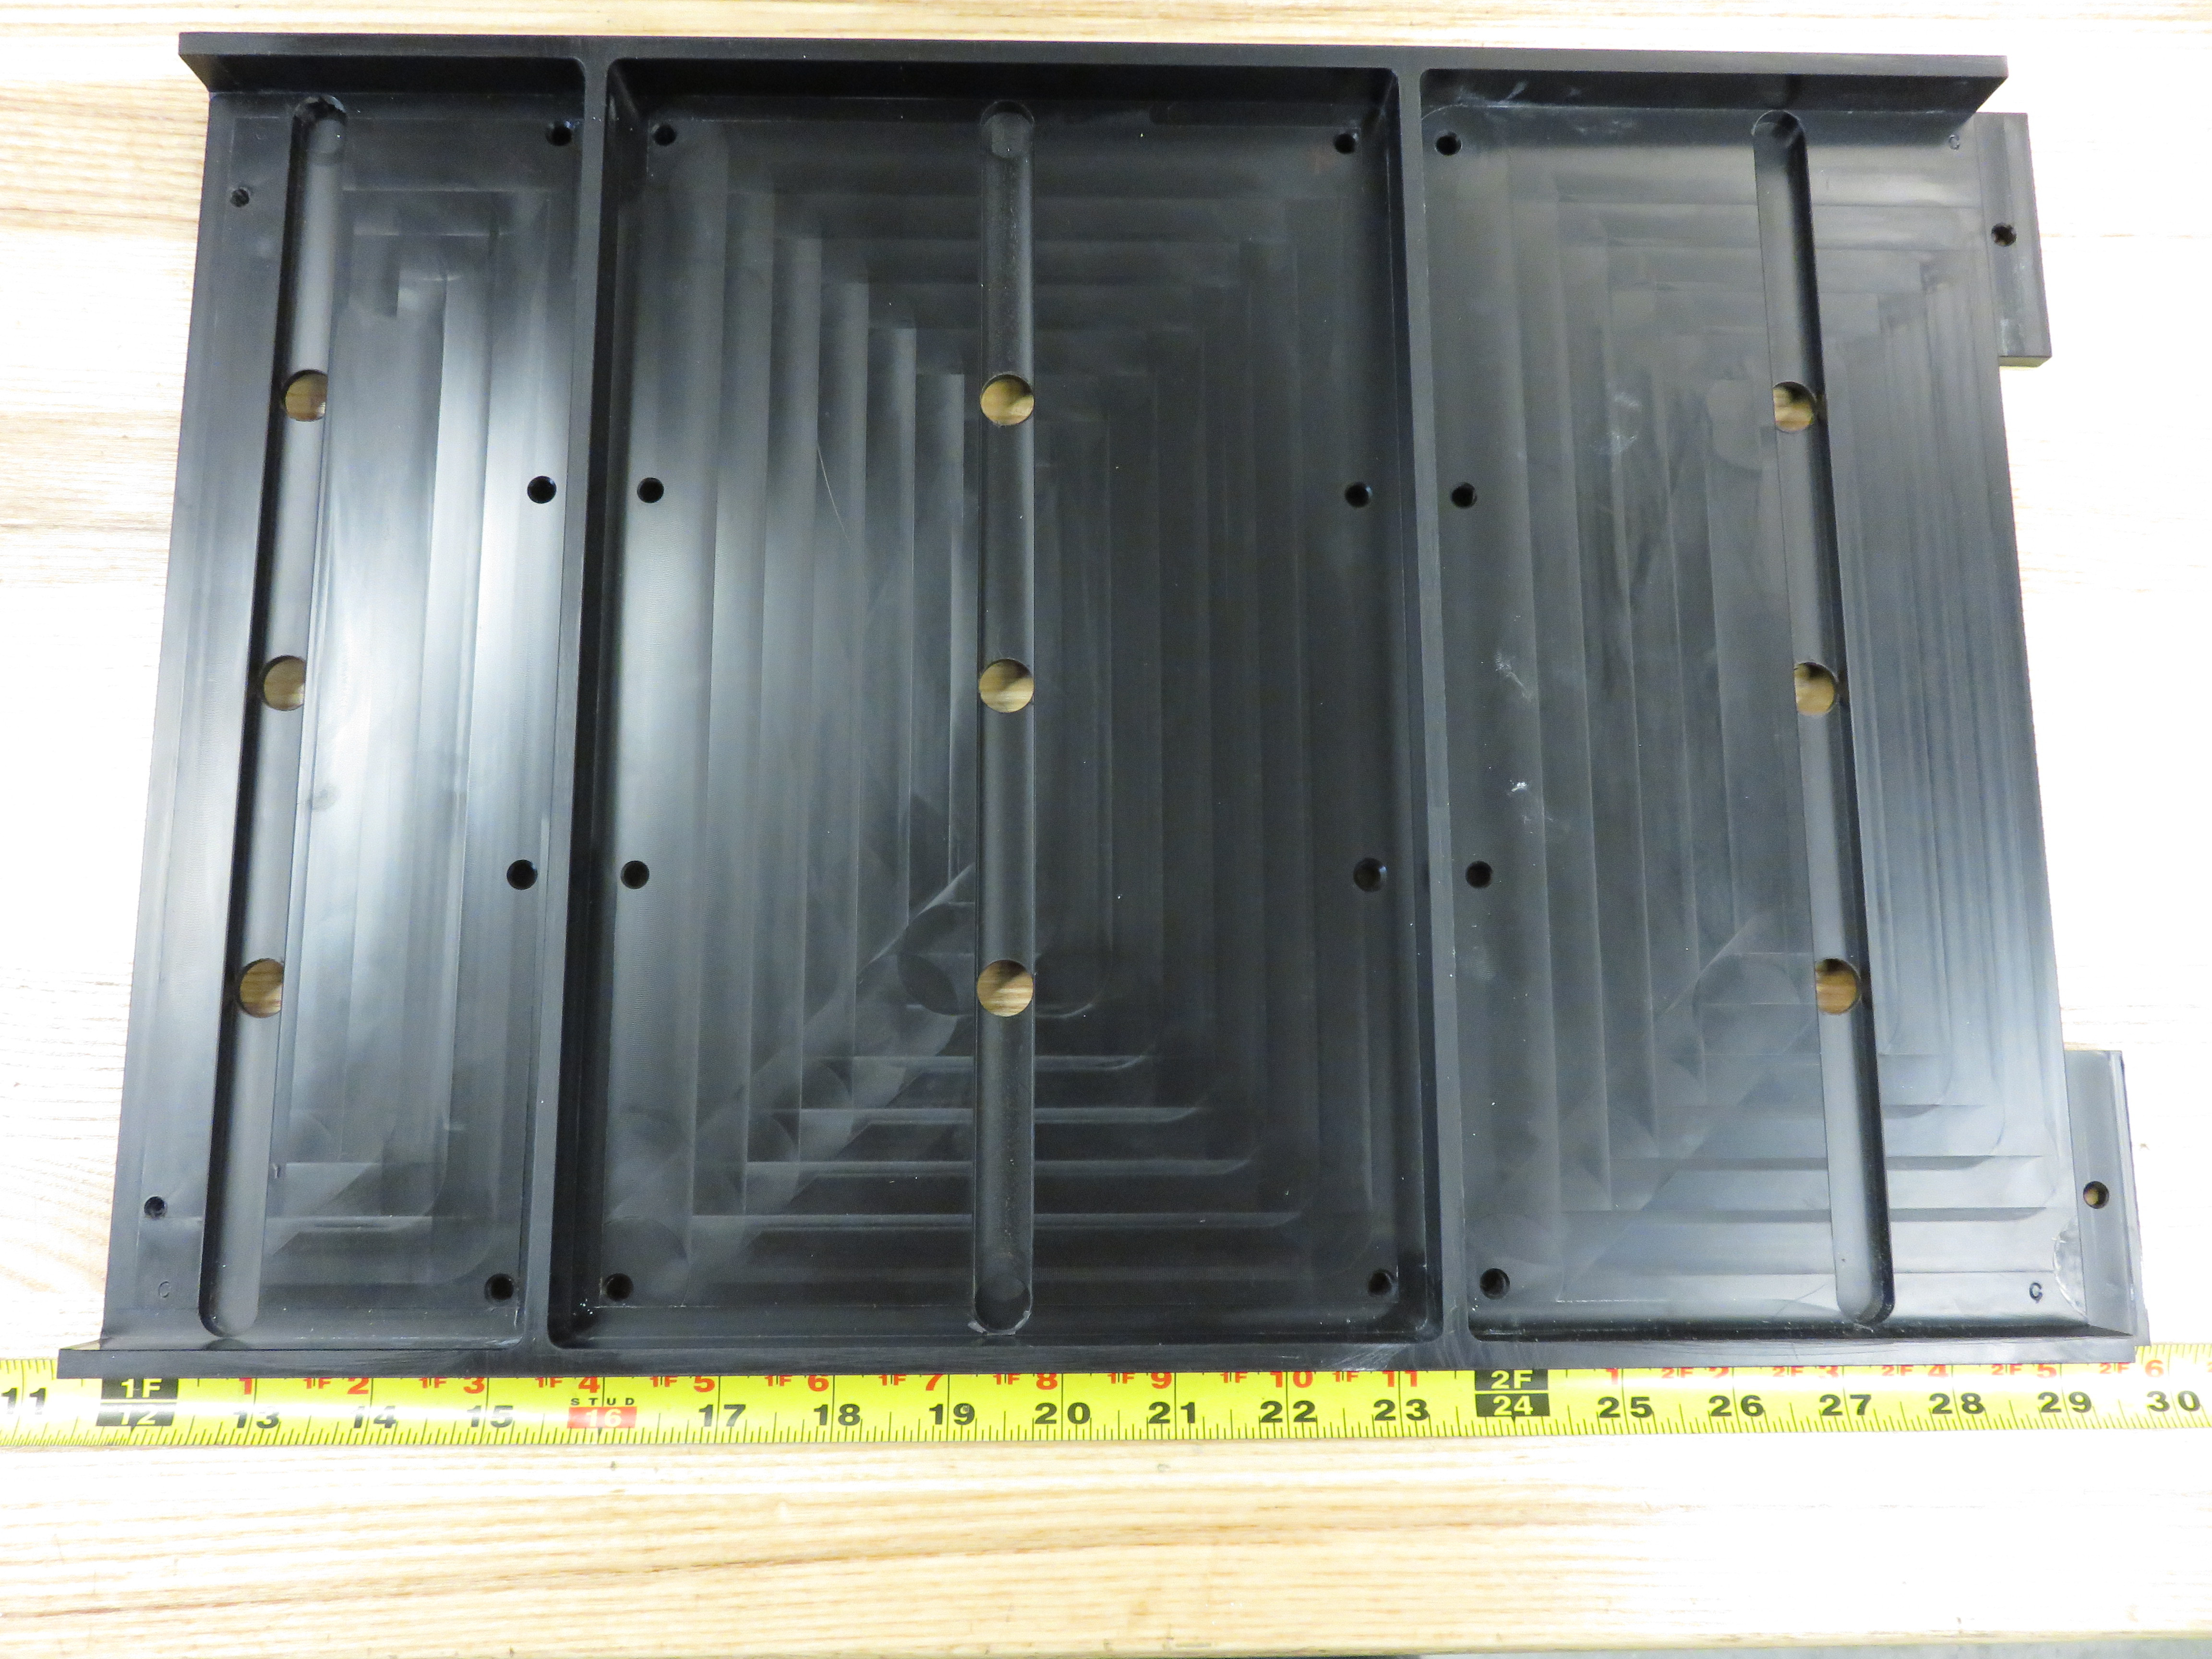
\includegraphics[scale=0.2]{facility/MachinedParts/C_meas_v2.JPG}}}
   {\subfigcapskip = 5pt \subfigcapmargin = -12pt  \subfigure[]{\label{fig:edge-b}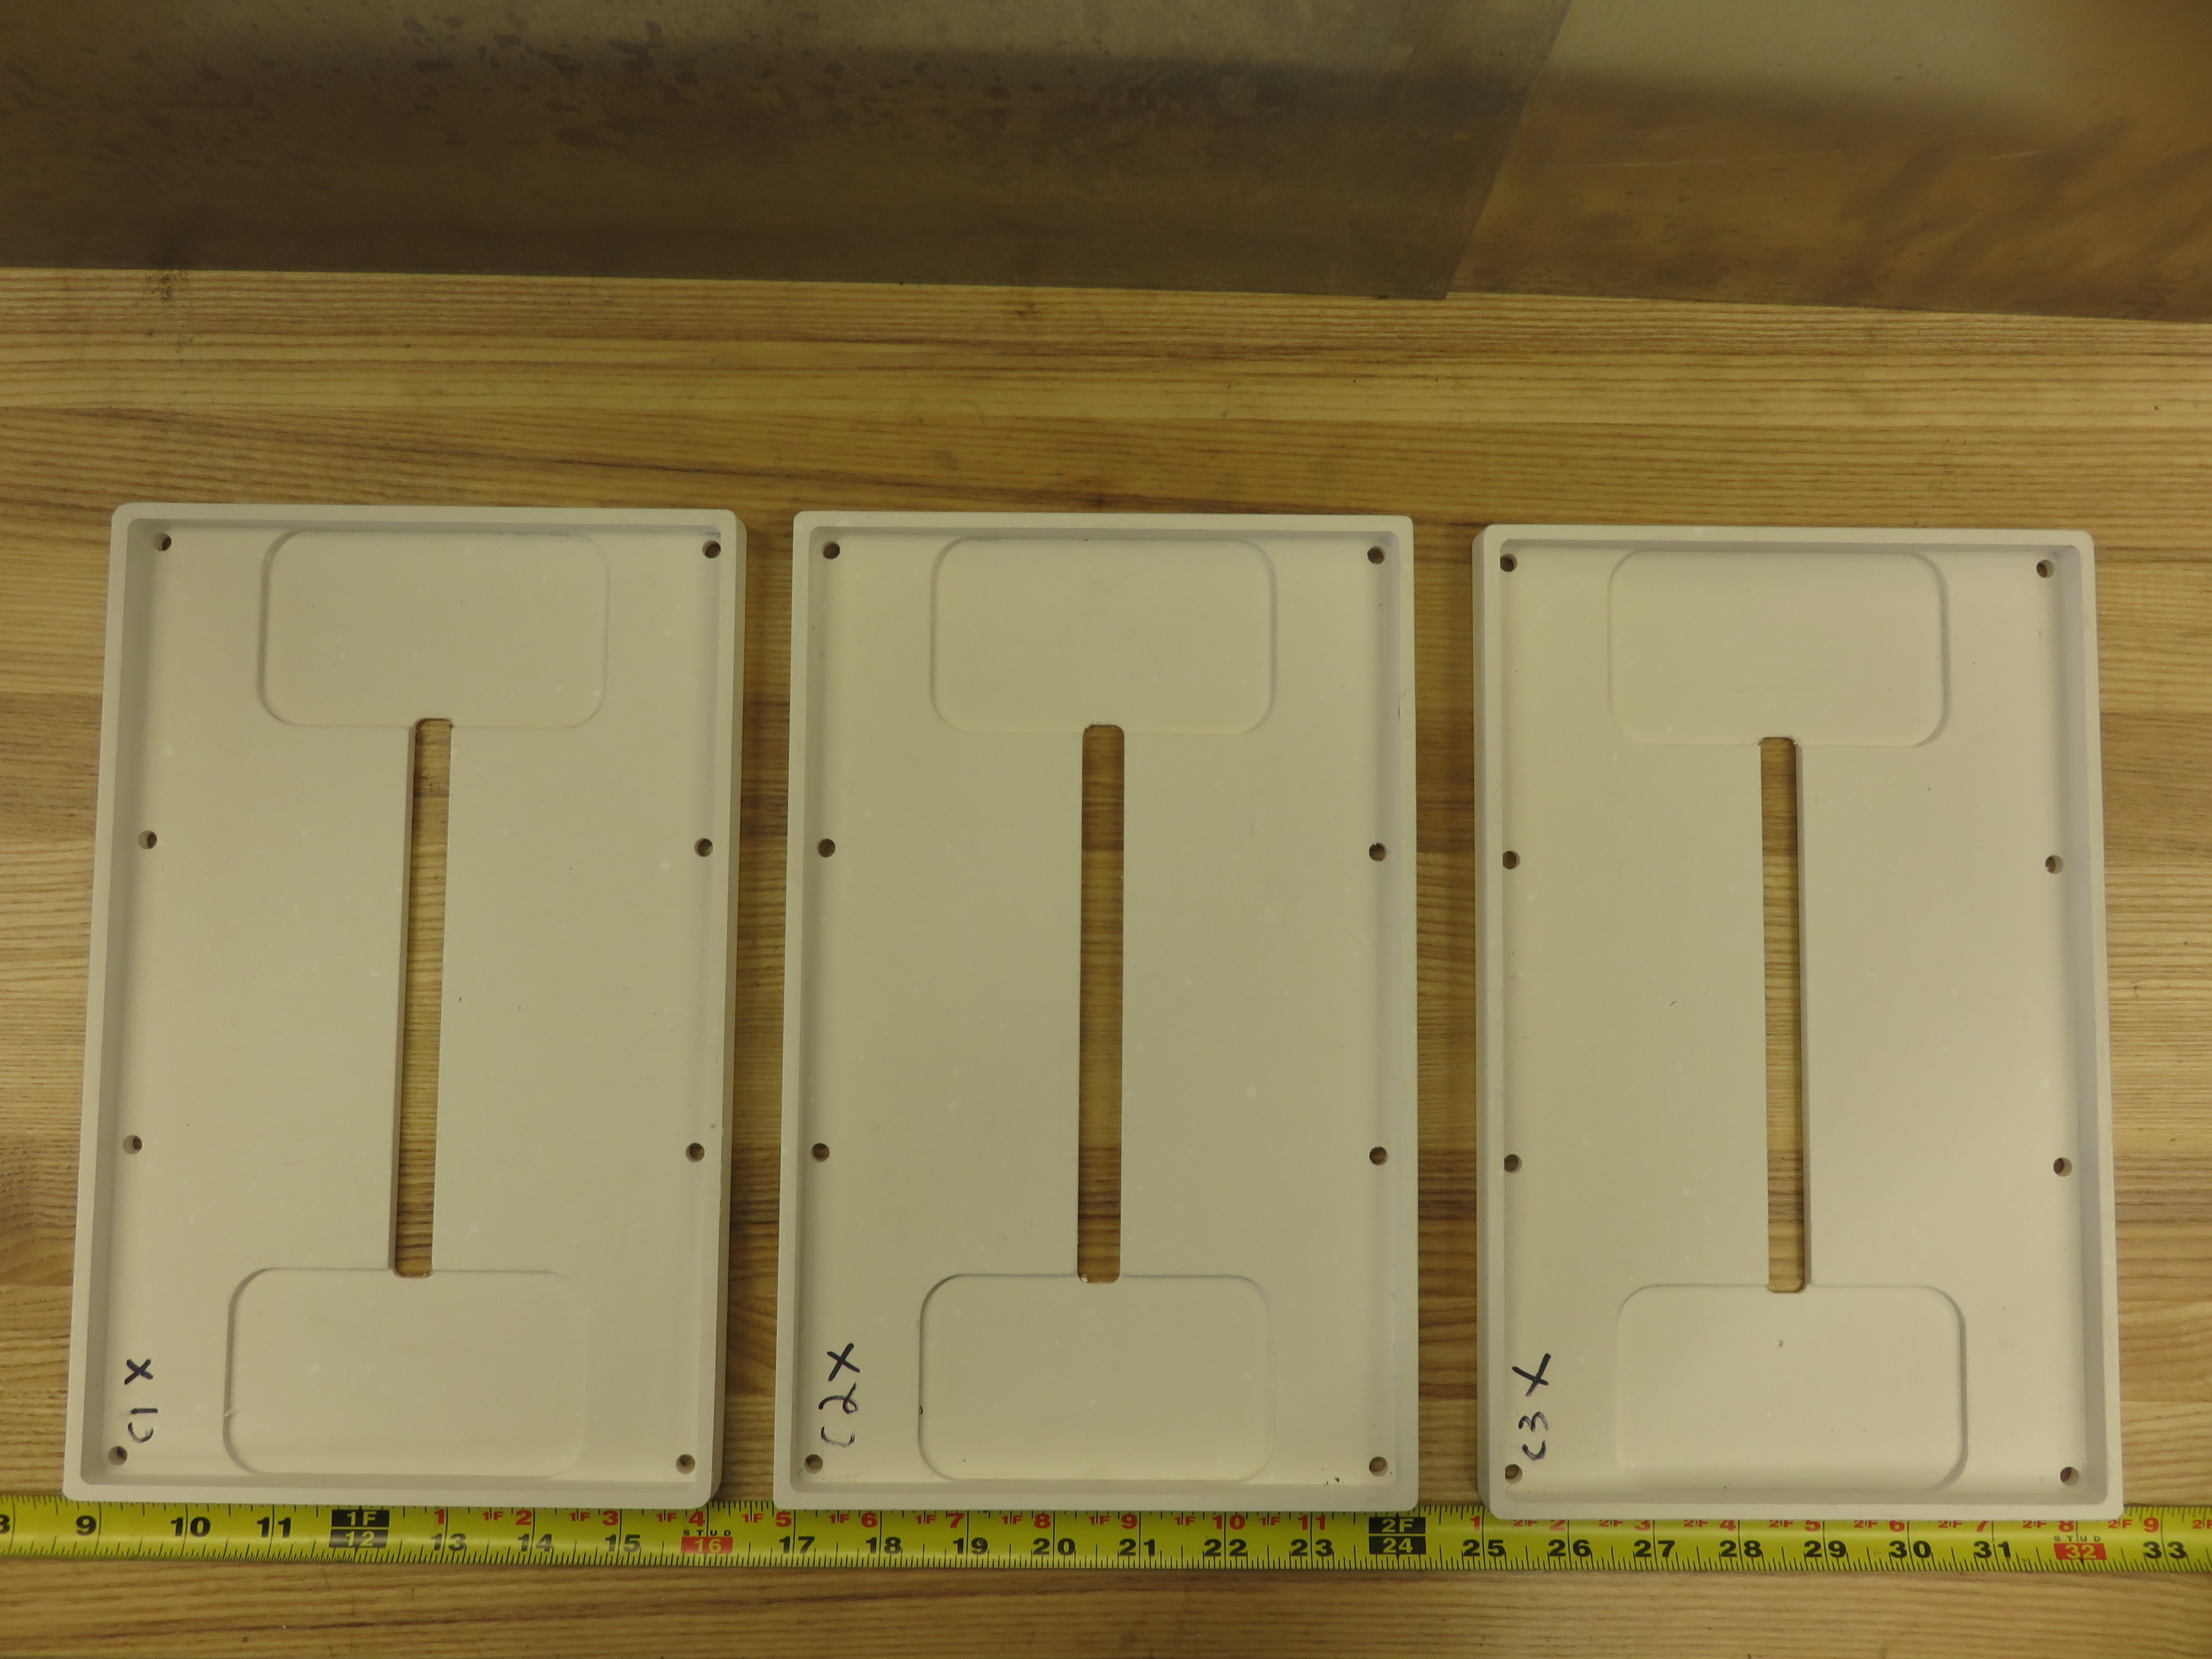
\includegraphics[scale=0.2]{facility/MachinedParts/C_insul_v1.JPG}}}
  \end{center}
\caption{(a) insulation (b) frame. } 
\end{figure}


%%%%%%%%%%%%%%%%%%%%%%%%%%%%%%%%%%%%%%%%%%%%%%%%%%%%%%
\clearpage
\subsection{Components D}
Input text description?\\

%components D
\begin{figure}[h!]
\centering
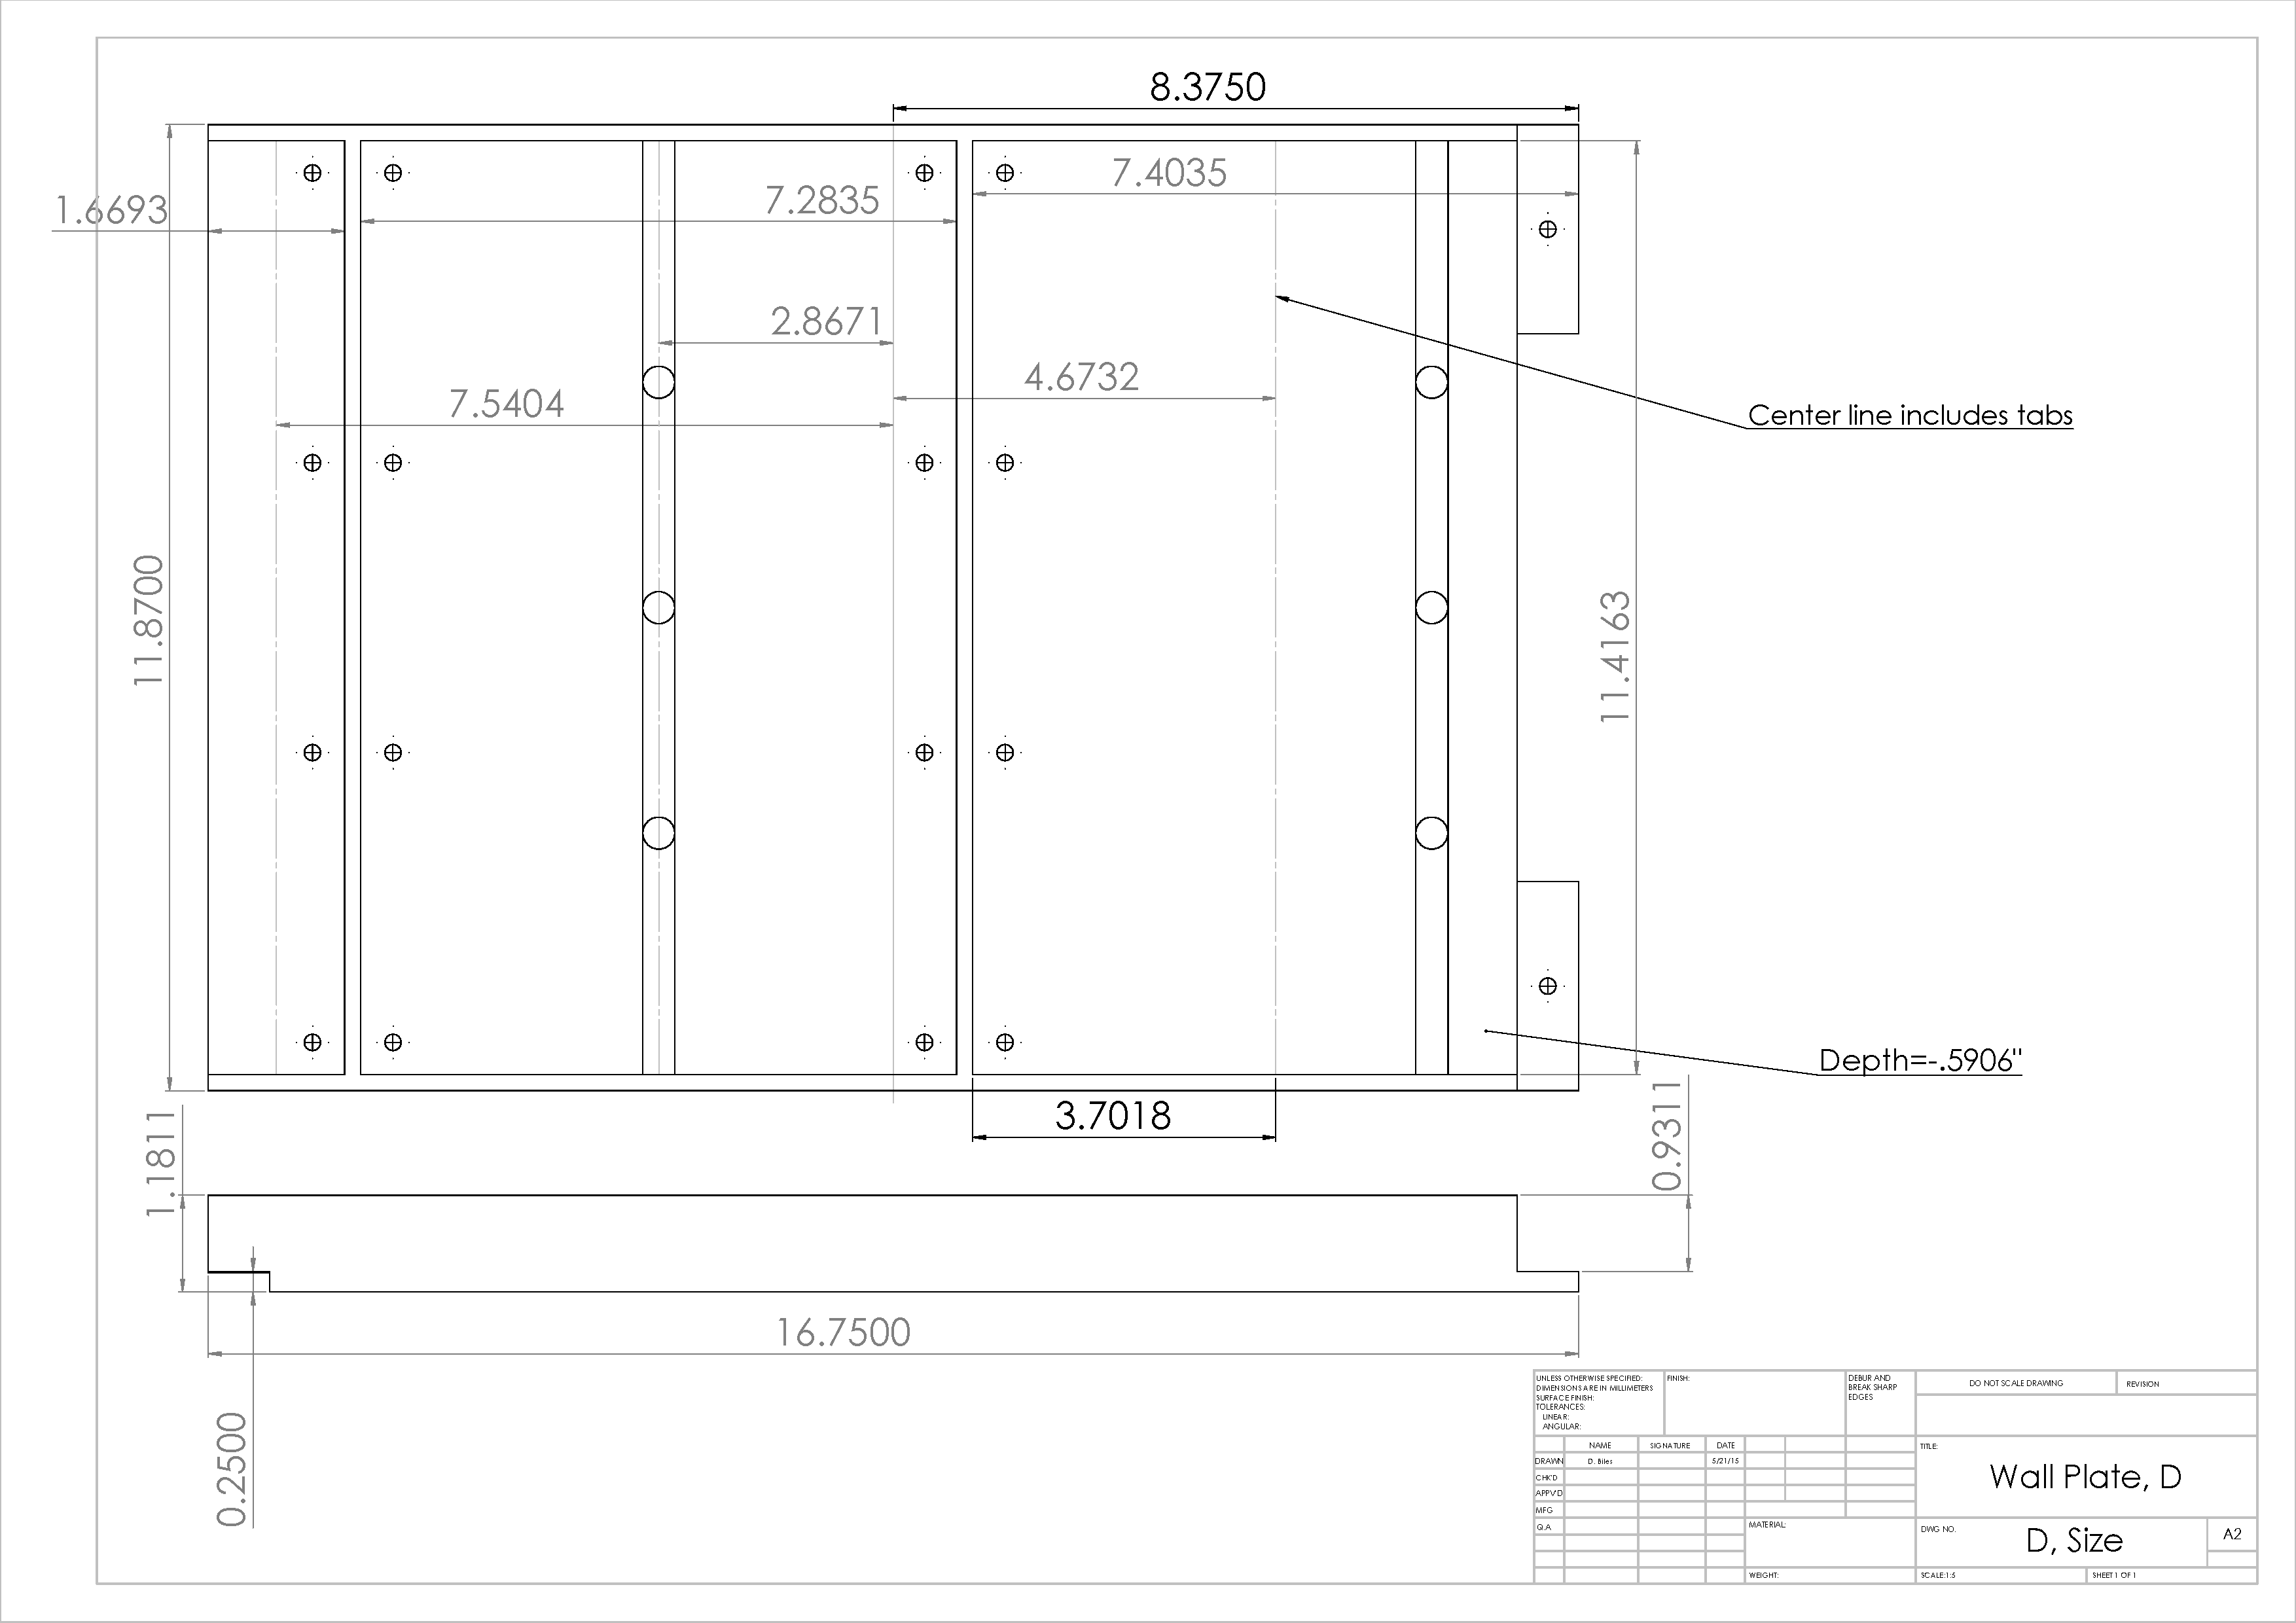
\includegraphics[scale=.2]{facility/drawings/D_size.PDF}
\caption{\footnotesize {\bf XX} } 
\end{figure}

\begin{figure}[h!]
\centering
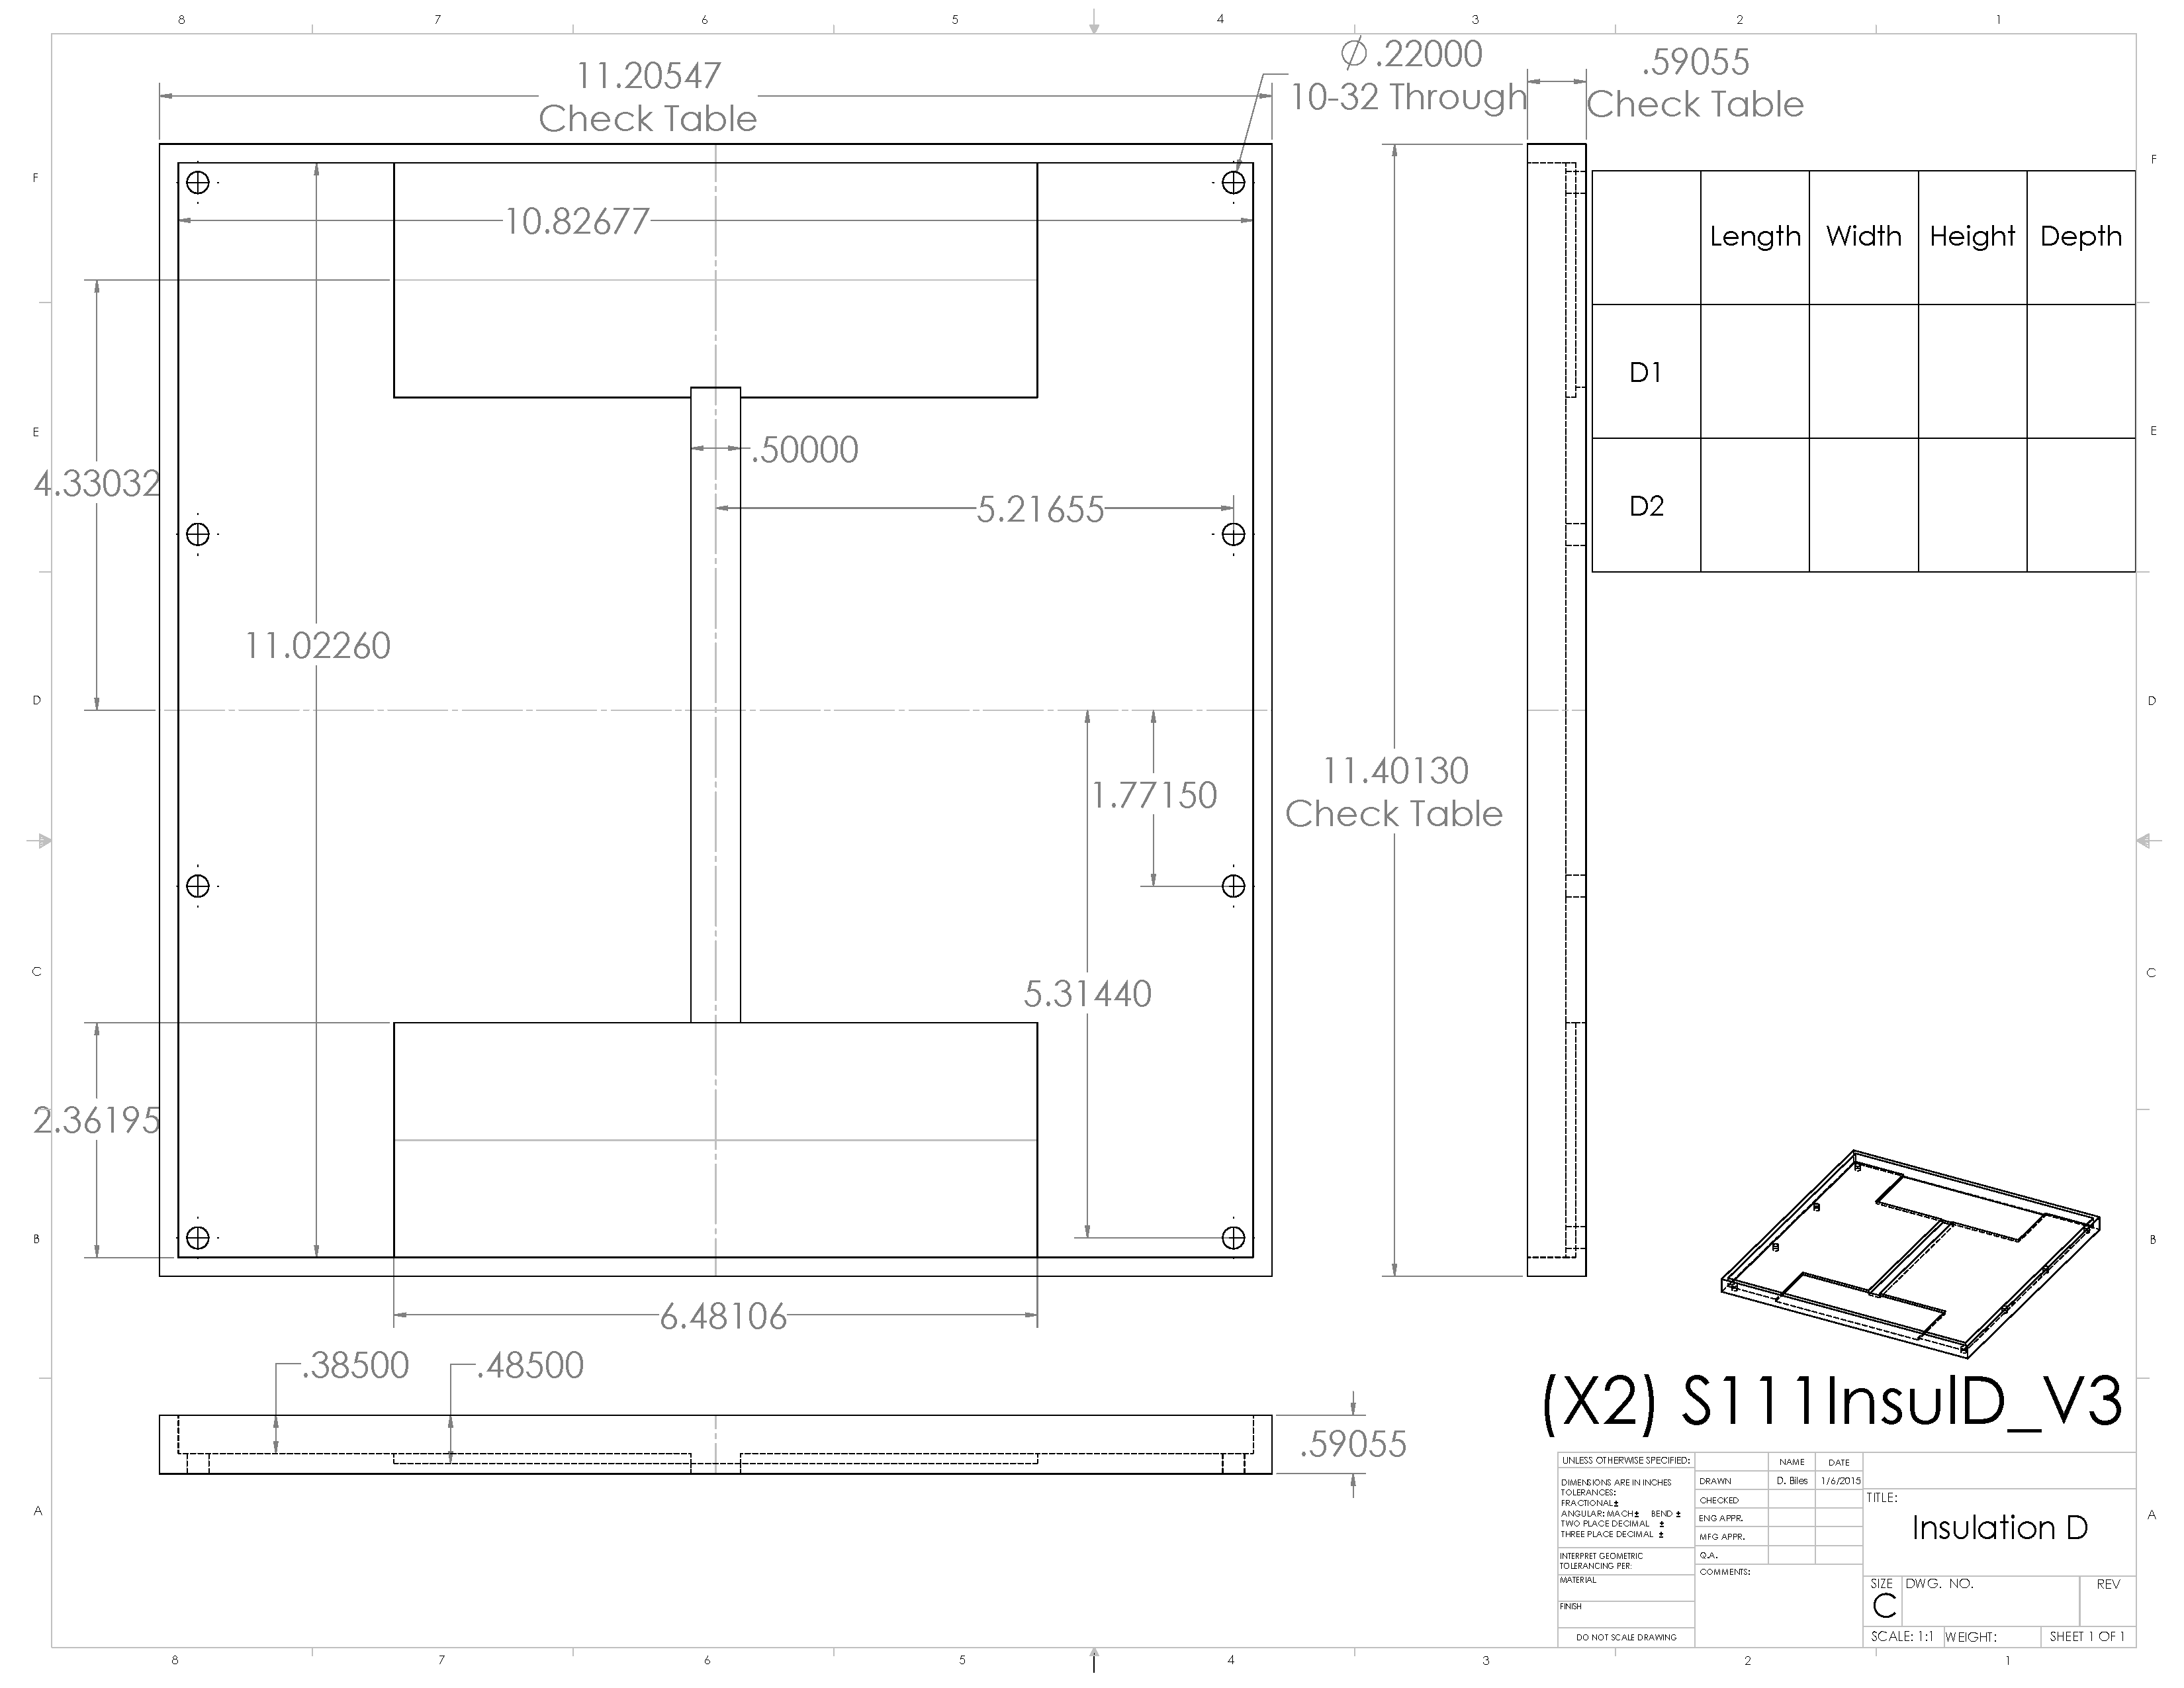
\includegraphics[scale=.2]{facility/drawings/Insulation_D.PDF}
\caption{\footnotesize {\bf XX} } 
\end{figure}

\begin{figure}[h!]
\centering
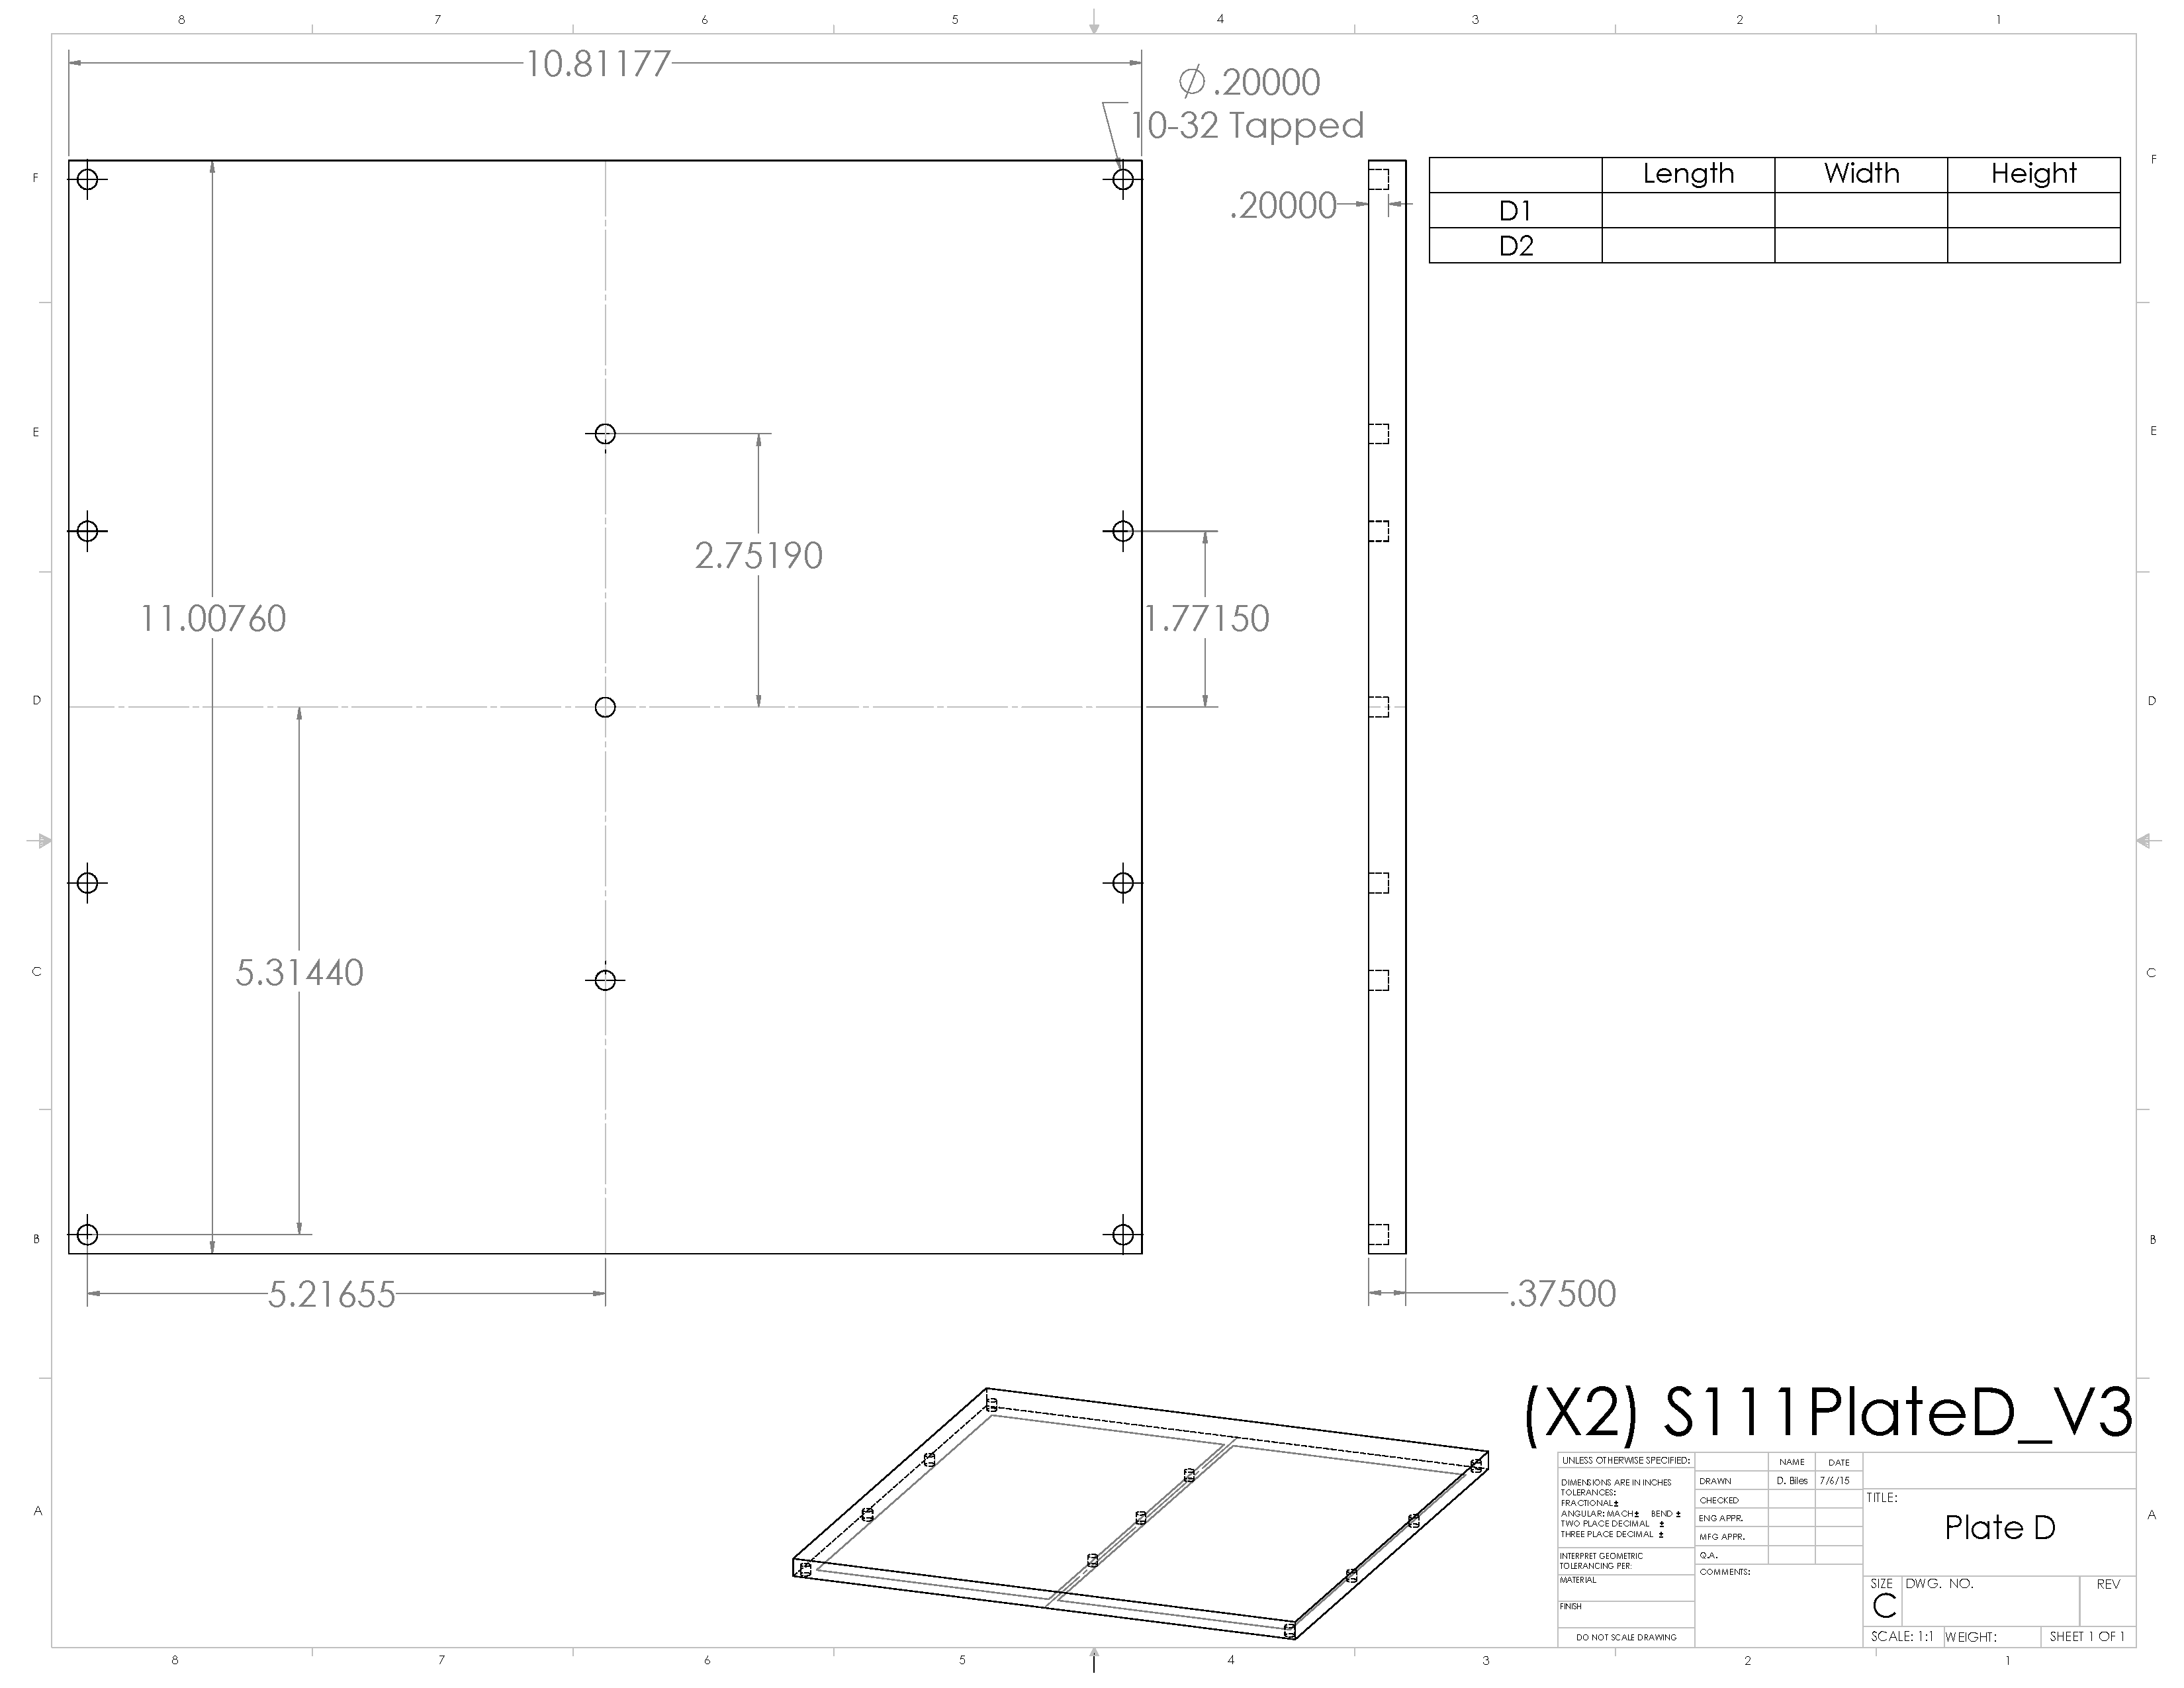
\includegraphics[scale=.2]{facility/drawings/Plate_D.PDF}
\caption{\footnotesize {\bf XX} } 
\end{figure}

\begin{figure}[h!]
  \begin{center}
  {\subfigcapskip = 5pt \subfigcapmargin = -12pt \subfigure[]{\label{fig:edge-a}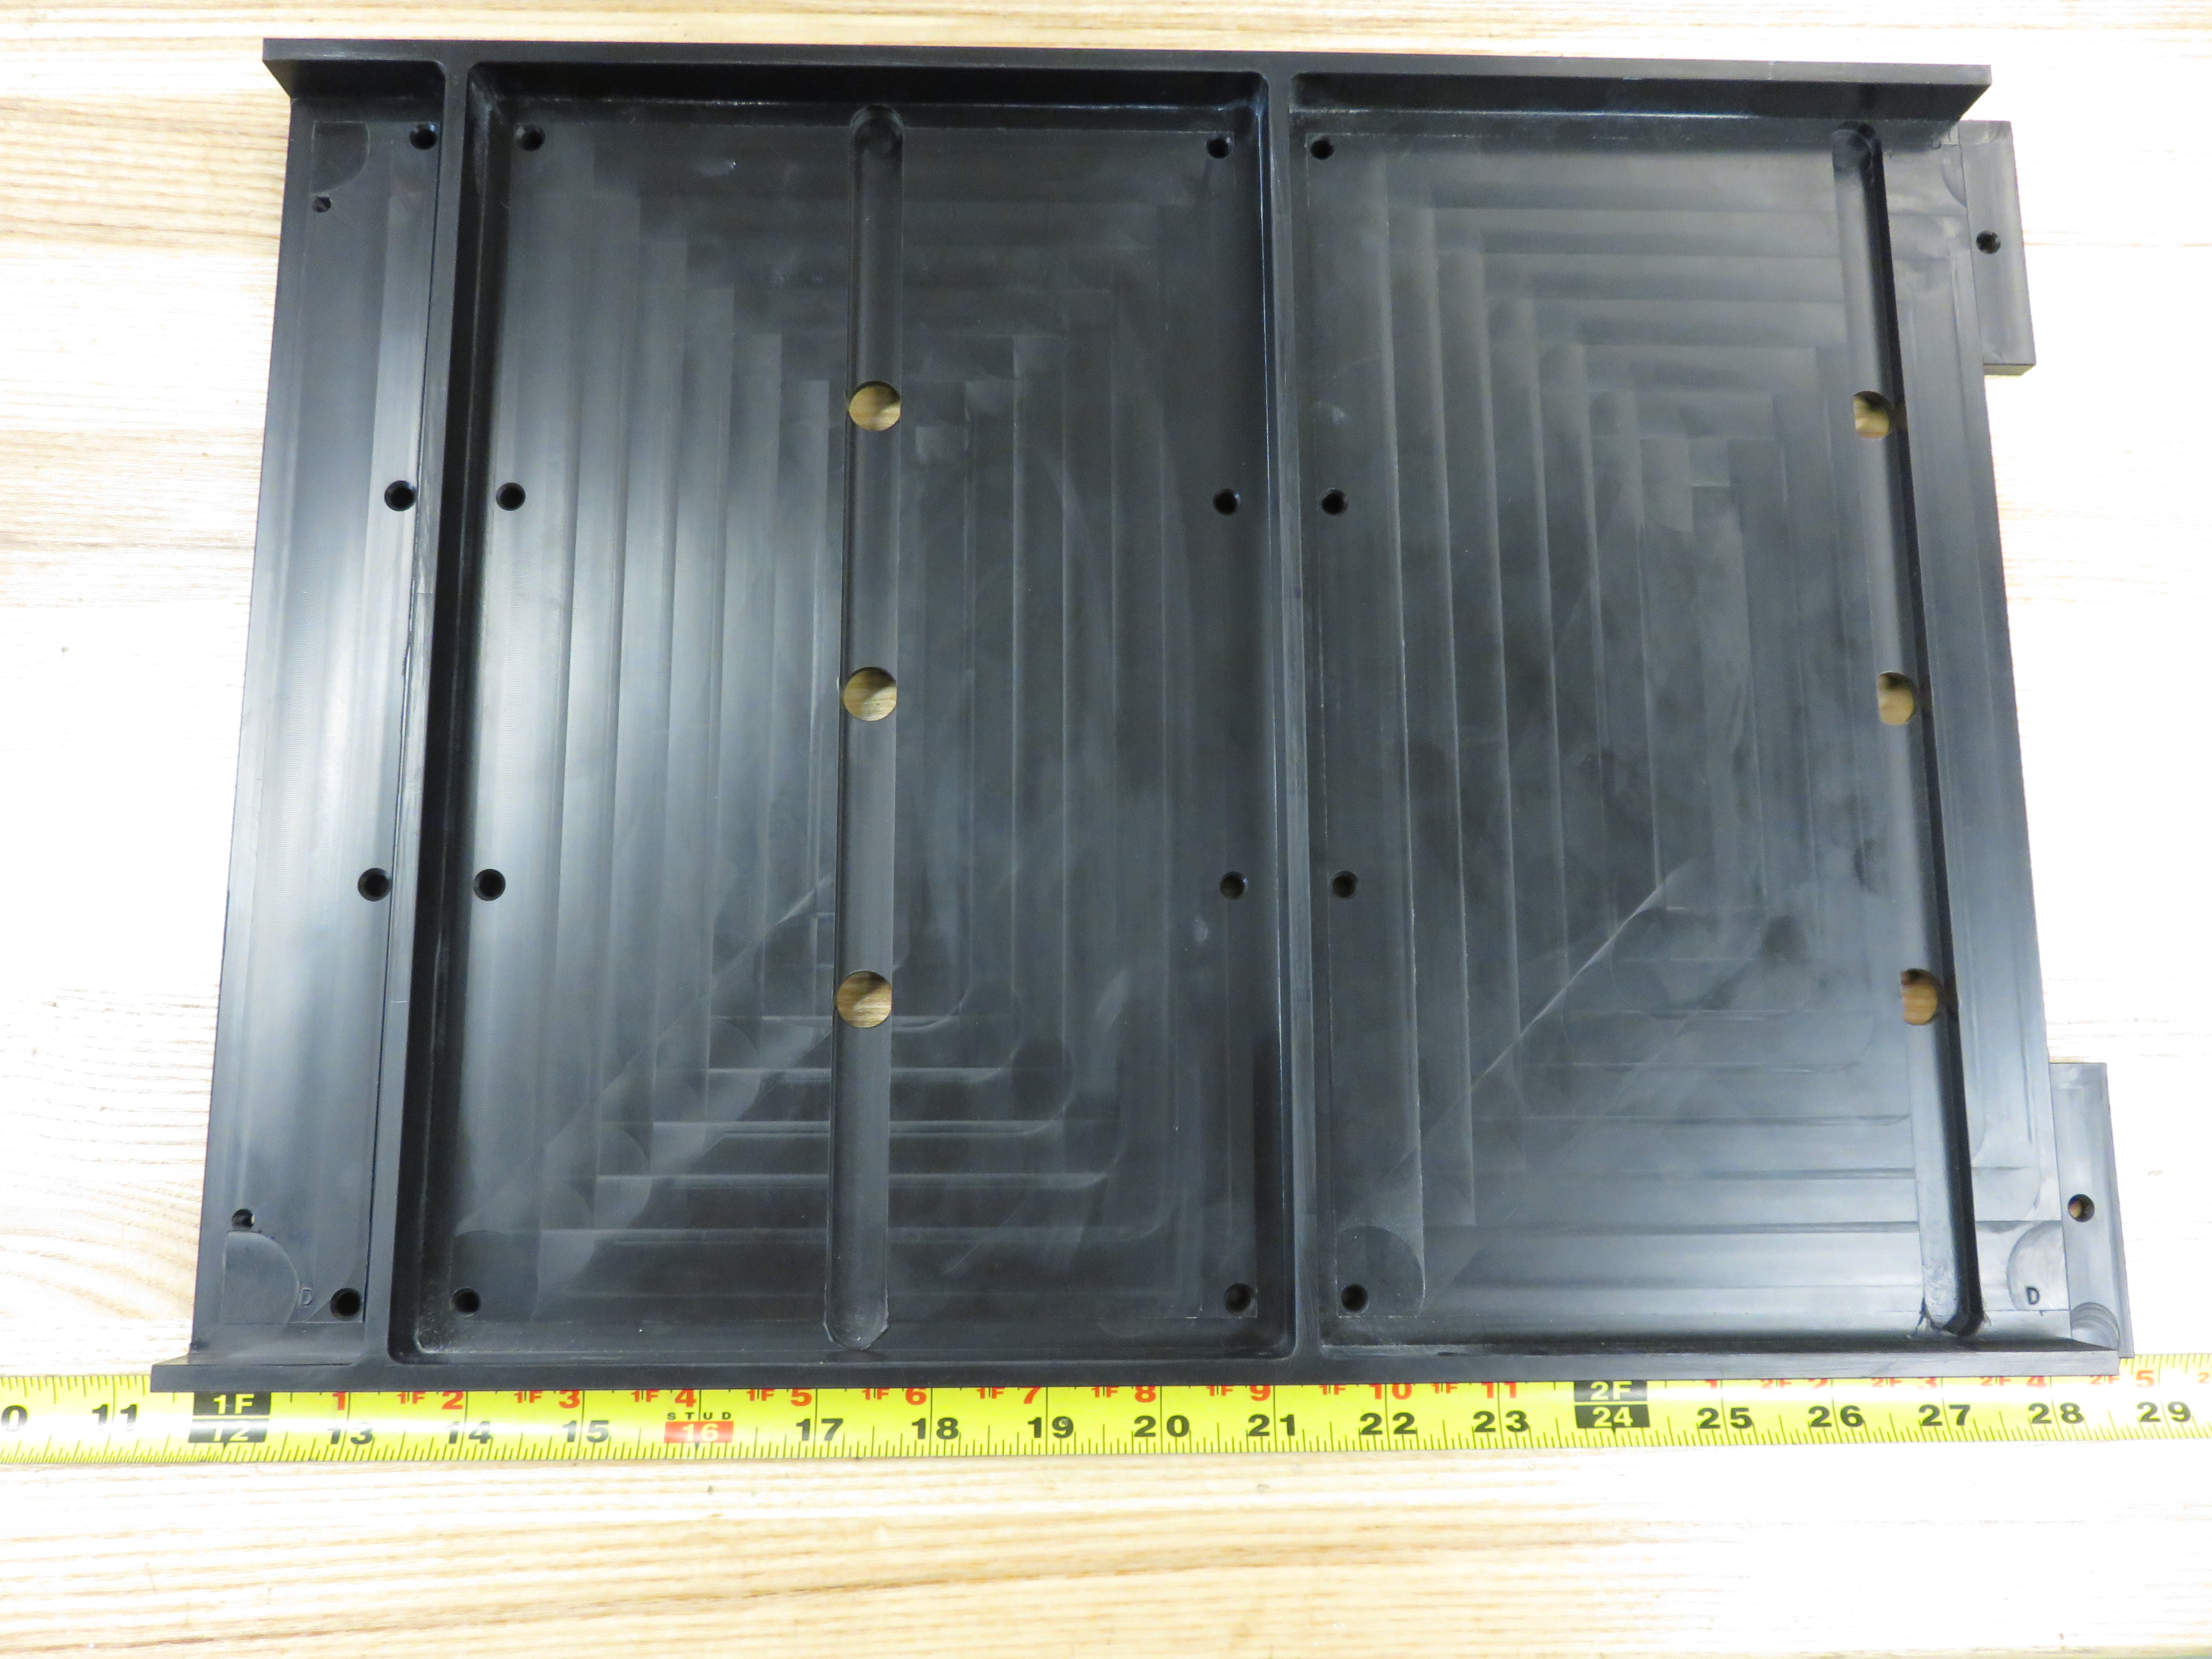
\includegraphics[scale=0.2]{facility/MachinedParts/D_meas_v2.JPG}}}
   {\subfigcapskip = 5pt \subfigcapmargin = -12pt  \subfigure[]{\label{fig:edge-b}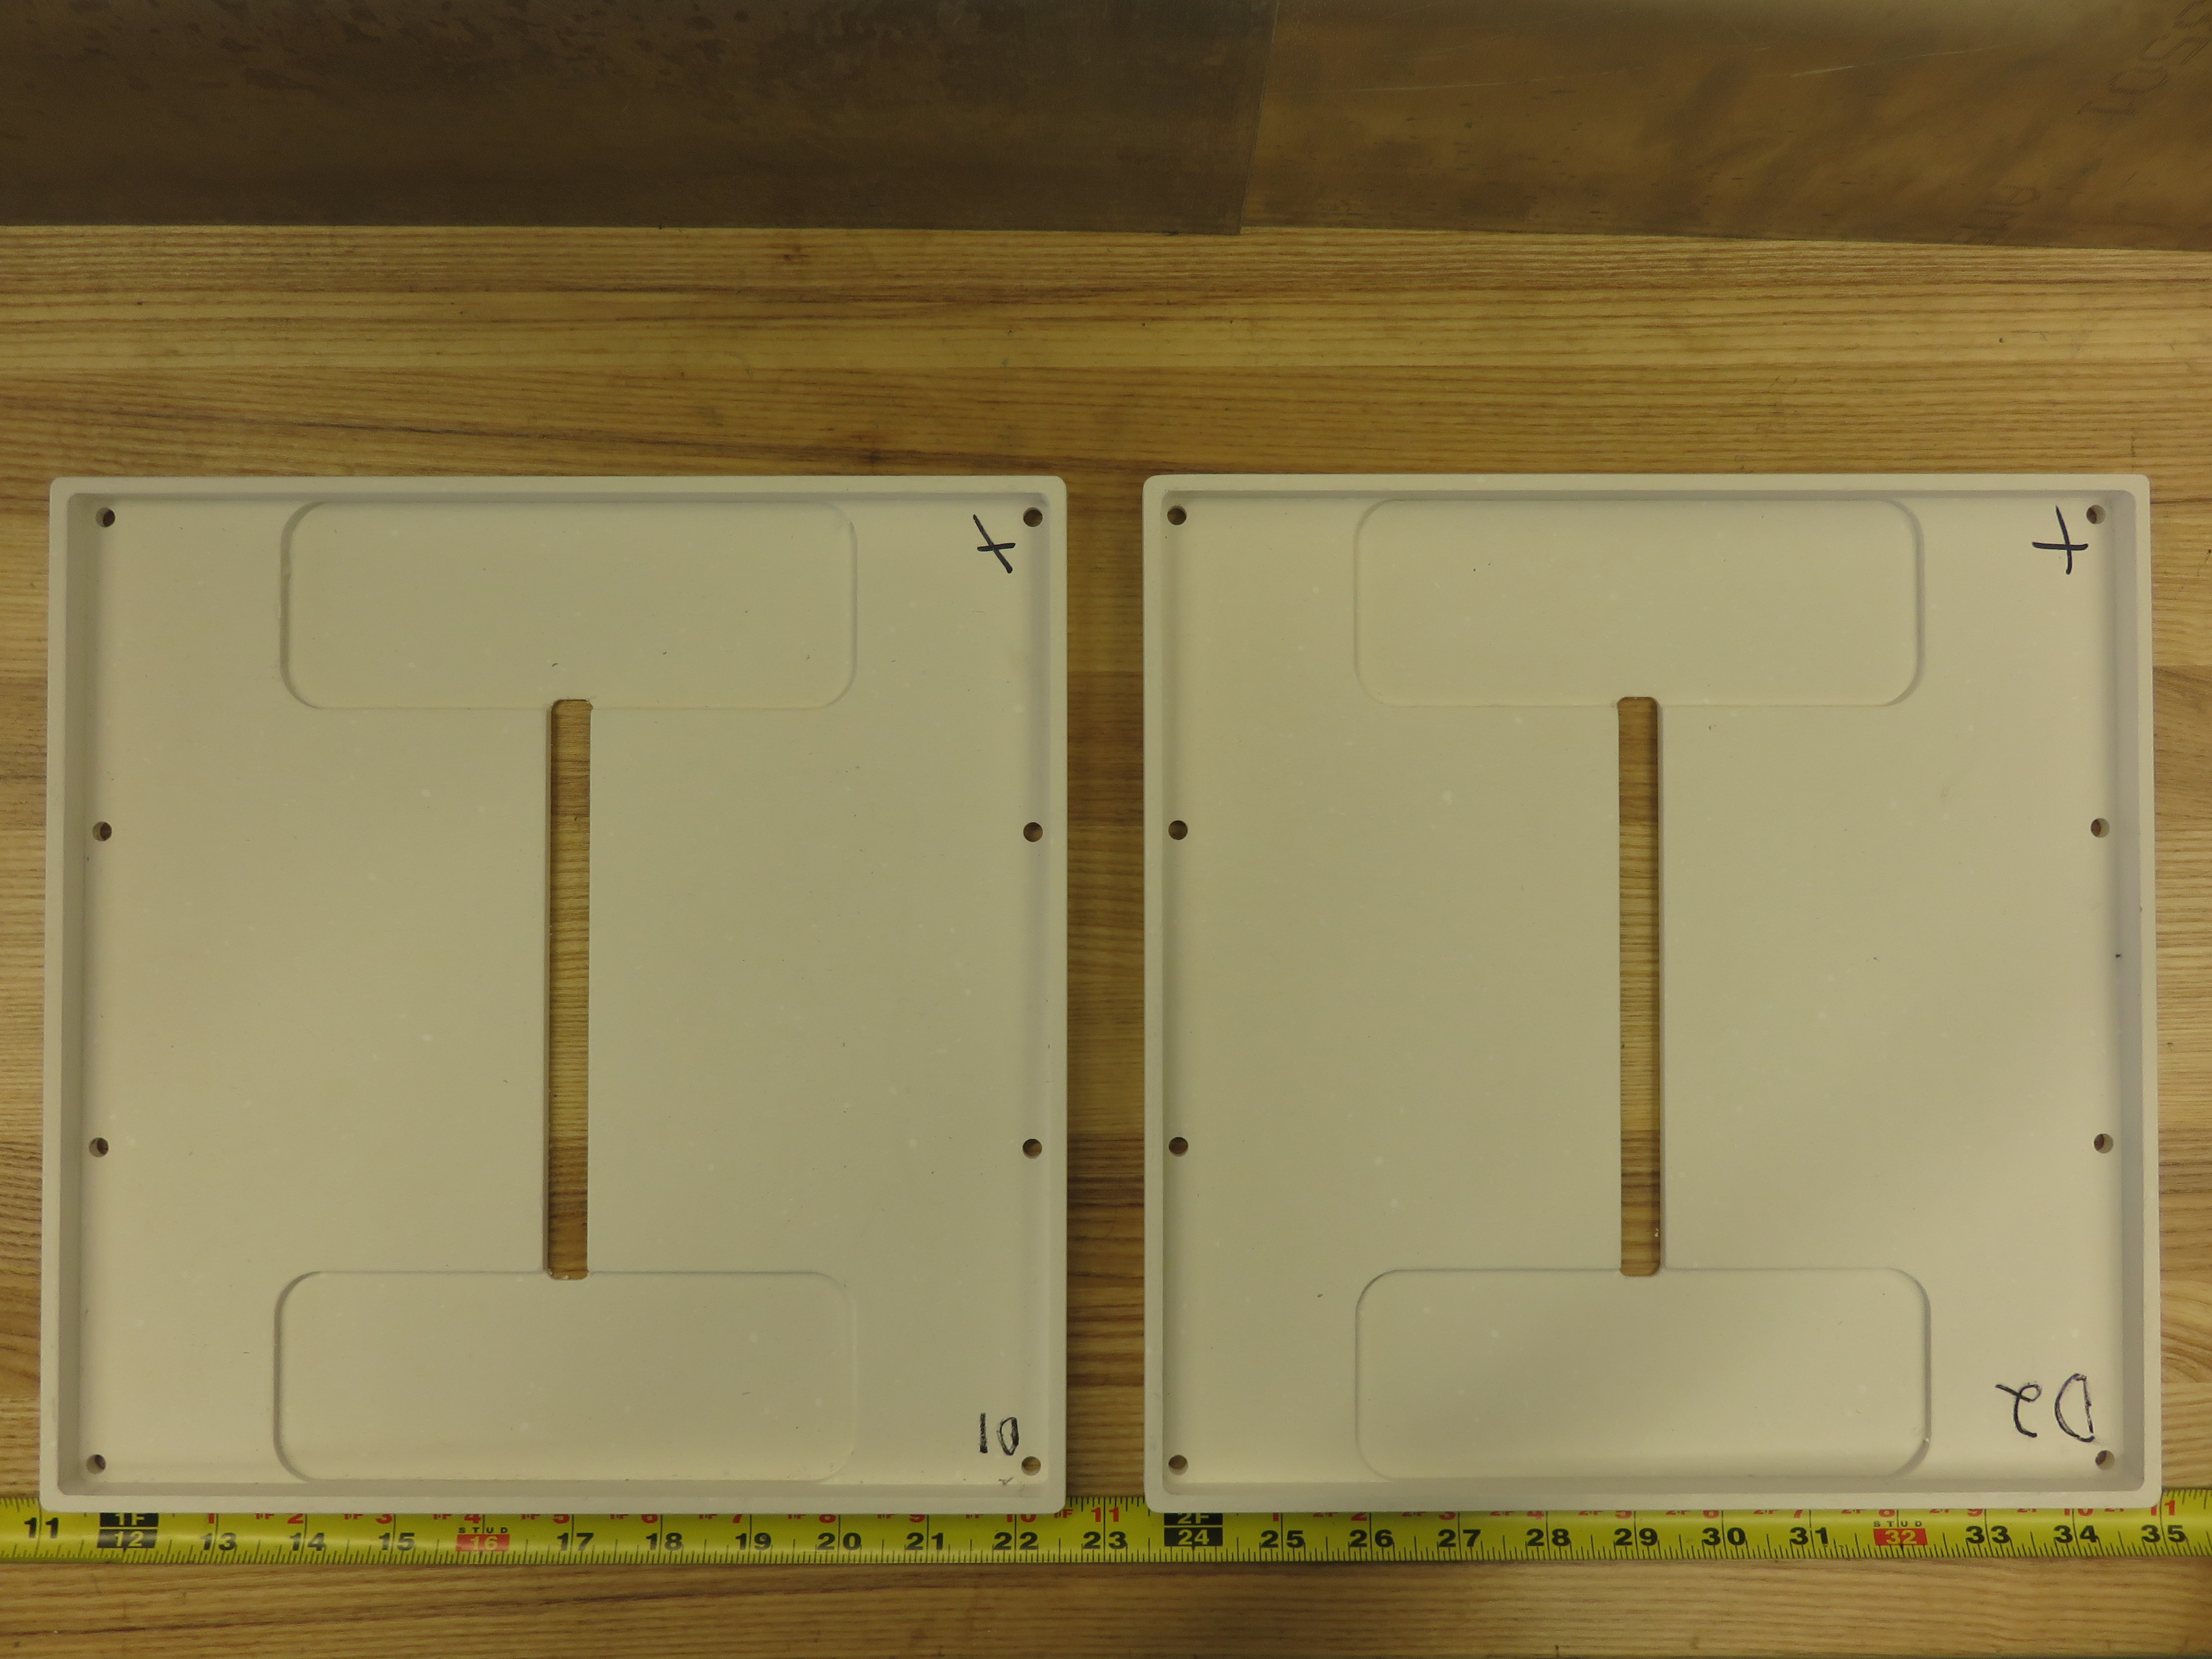
\includegraphics[scale=0.2]{facility/MachinedParts/D_insul_v2.JPG}}}
  \end{center}
\caption{(a) insulation (b) frame. } 
\end{figure}

%%%%%%%%%%%%%%%%%%%%%%%%%%%%%%%%%%%%%%%%%%%%%%%%%%%%%%
\clearpage
\subsection{Components E}
Input text description?\\

%components E
\begin{figure}[h!]
\centering
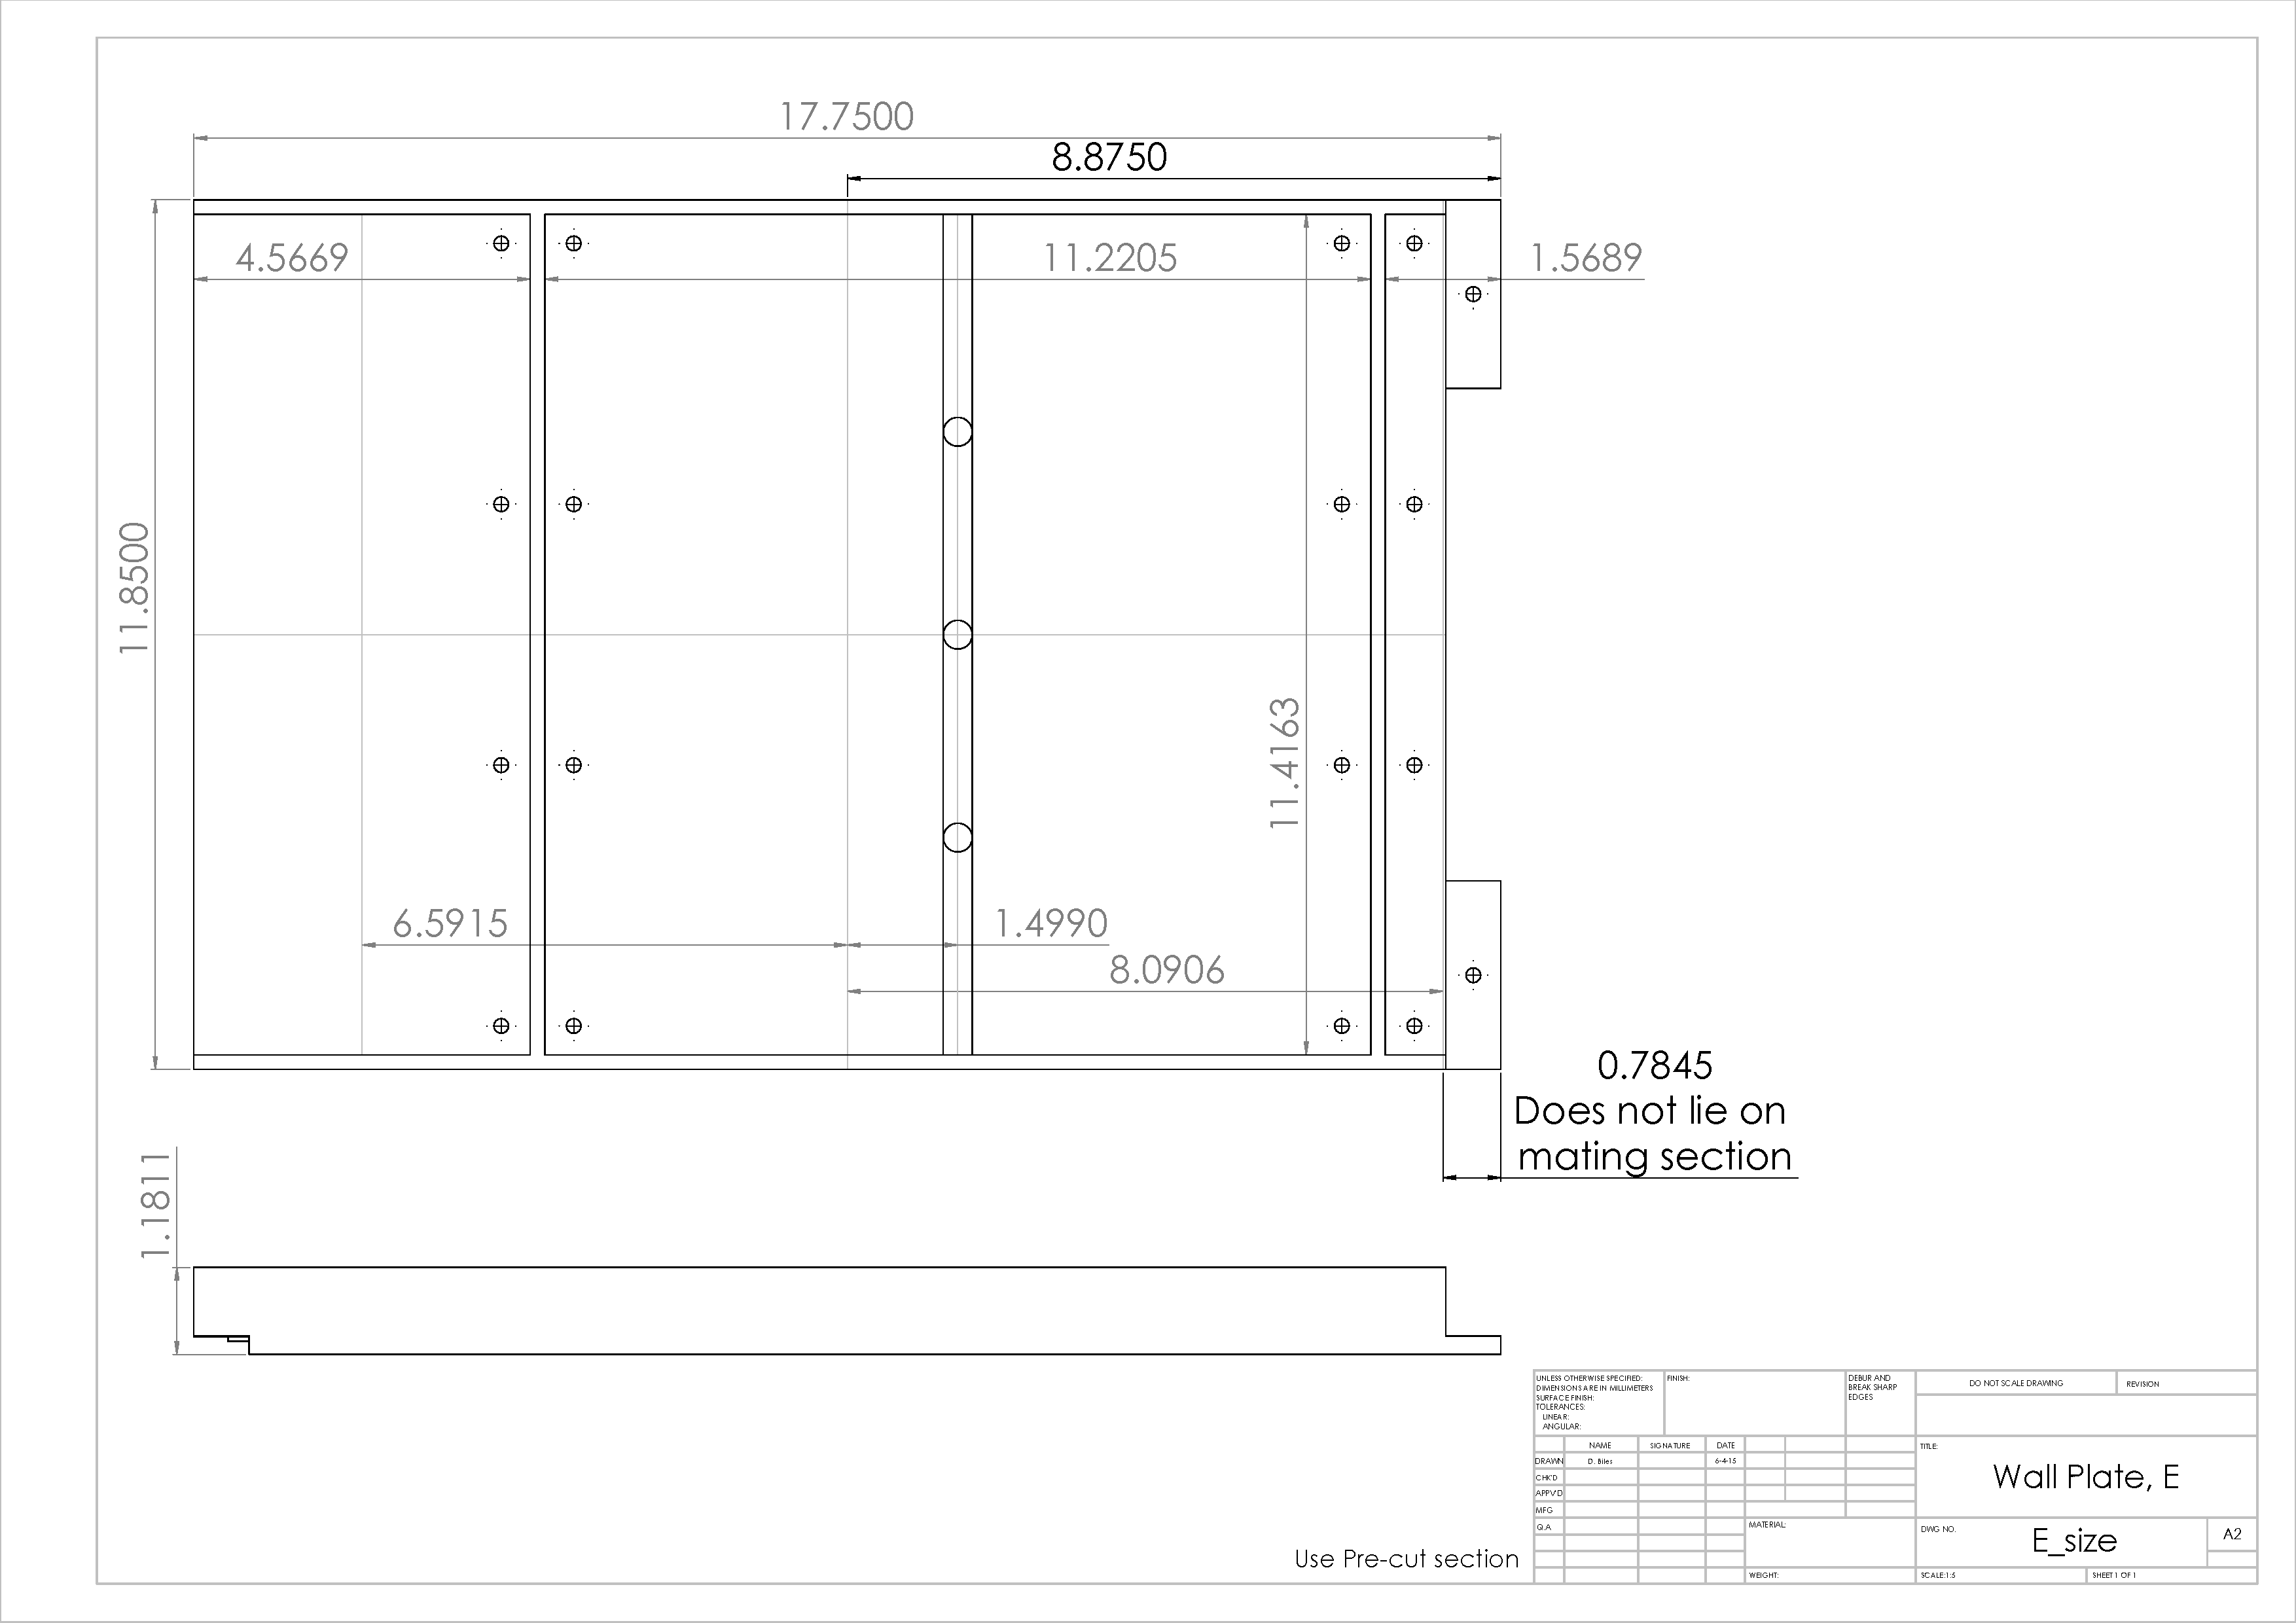
\includegraphics[scale=.2]{facility/drawings/E_size.PDF}
\caption{\footnotesize {\bf XX} } 
\end{figure}

\begin{figure}[h!]
\centering
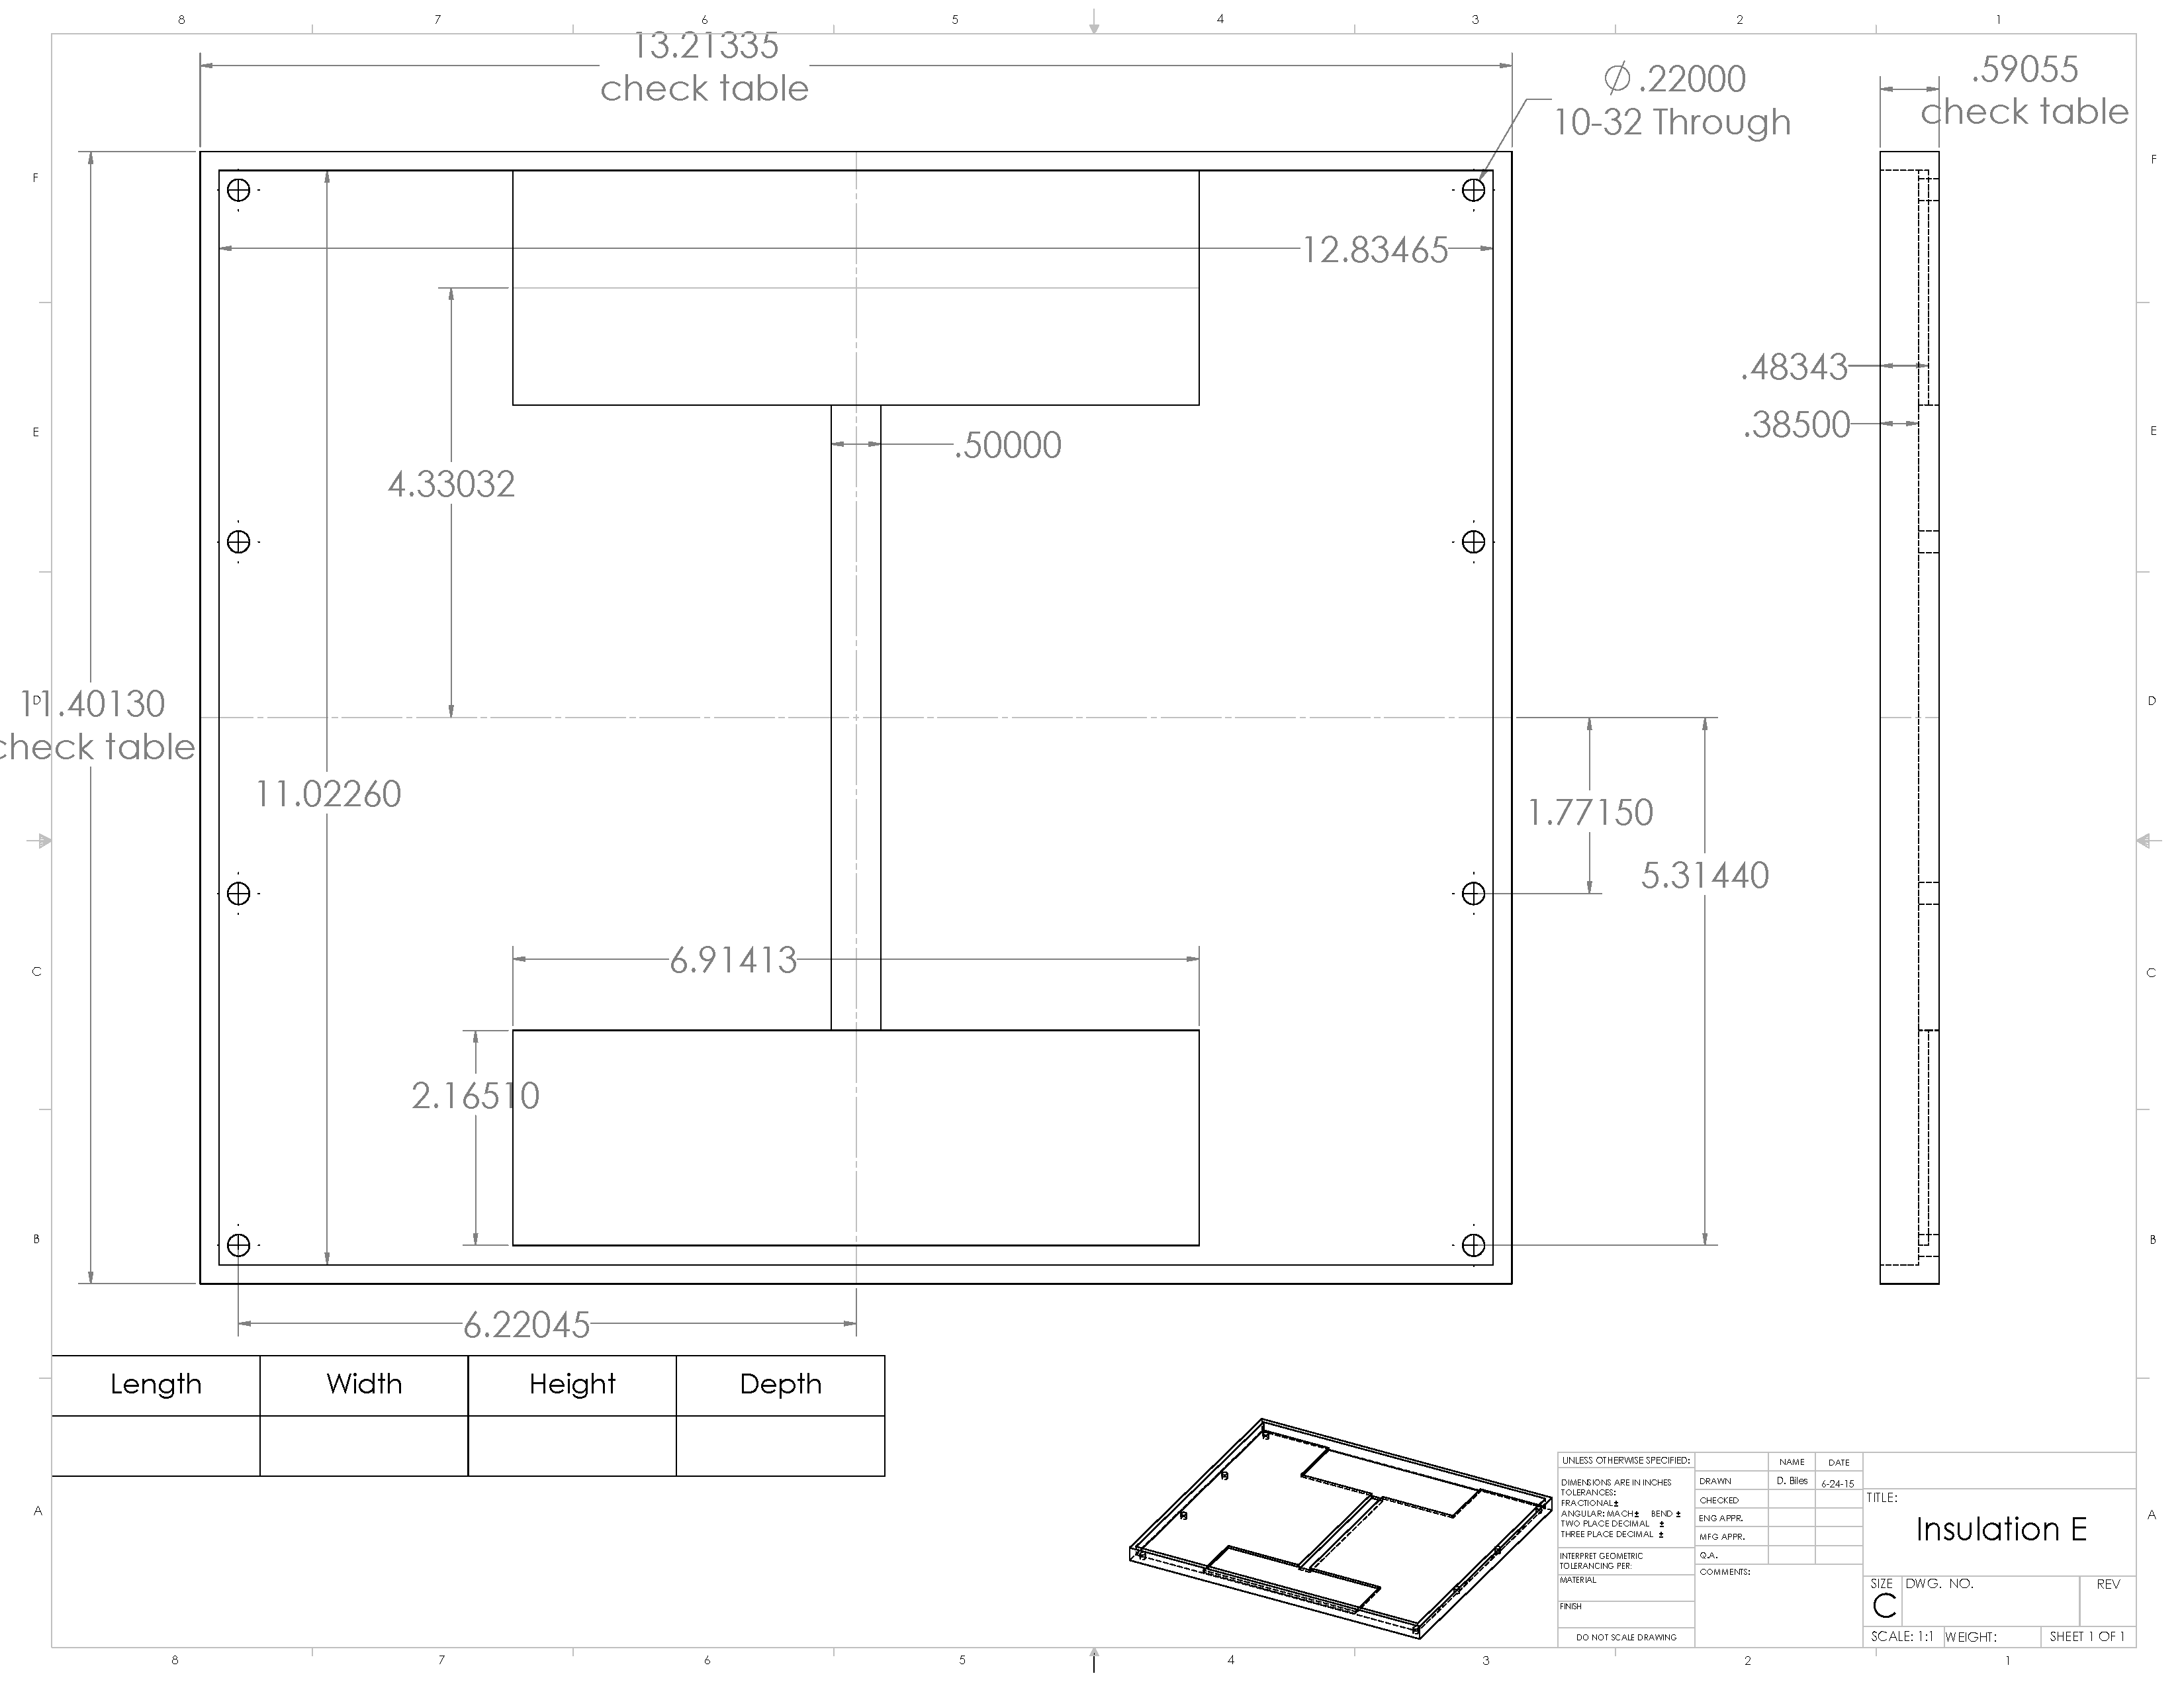
\includegraphics[scale=.2]{facility/drawings/Insulation_E.PDF}
\caption{\footnotesize {\bf XX} } 
\end{figure}

\begin{figure}[h!]
\centering
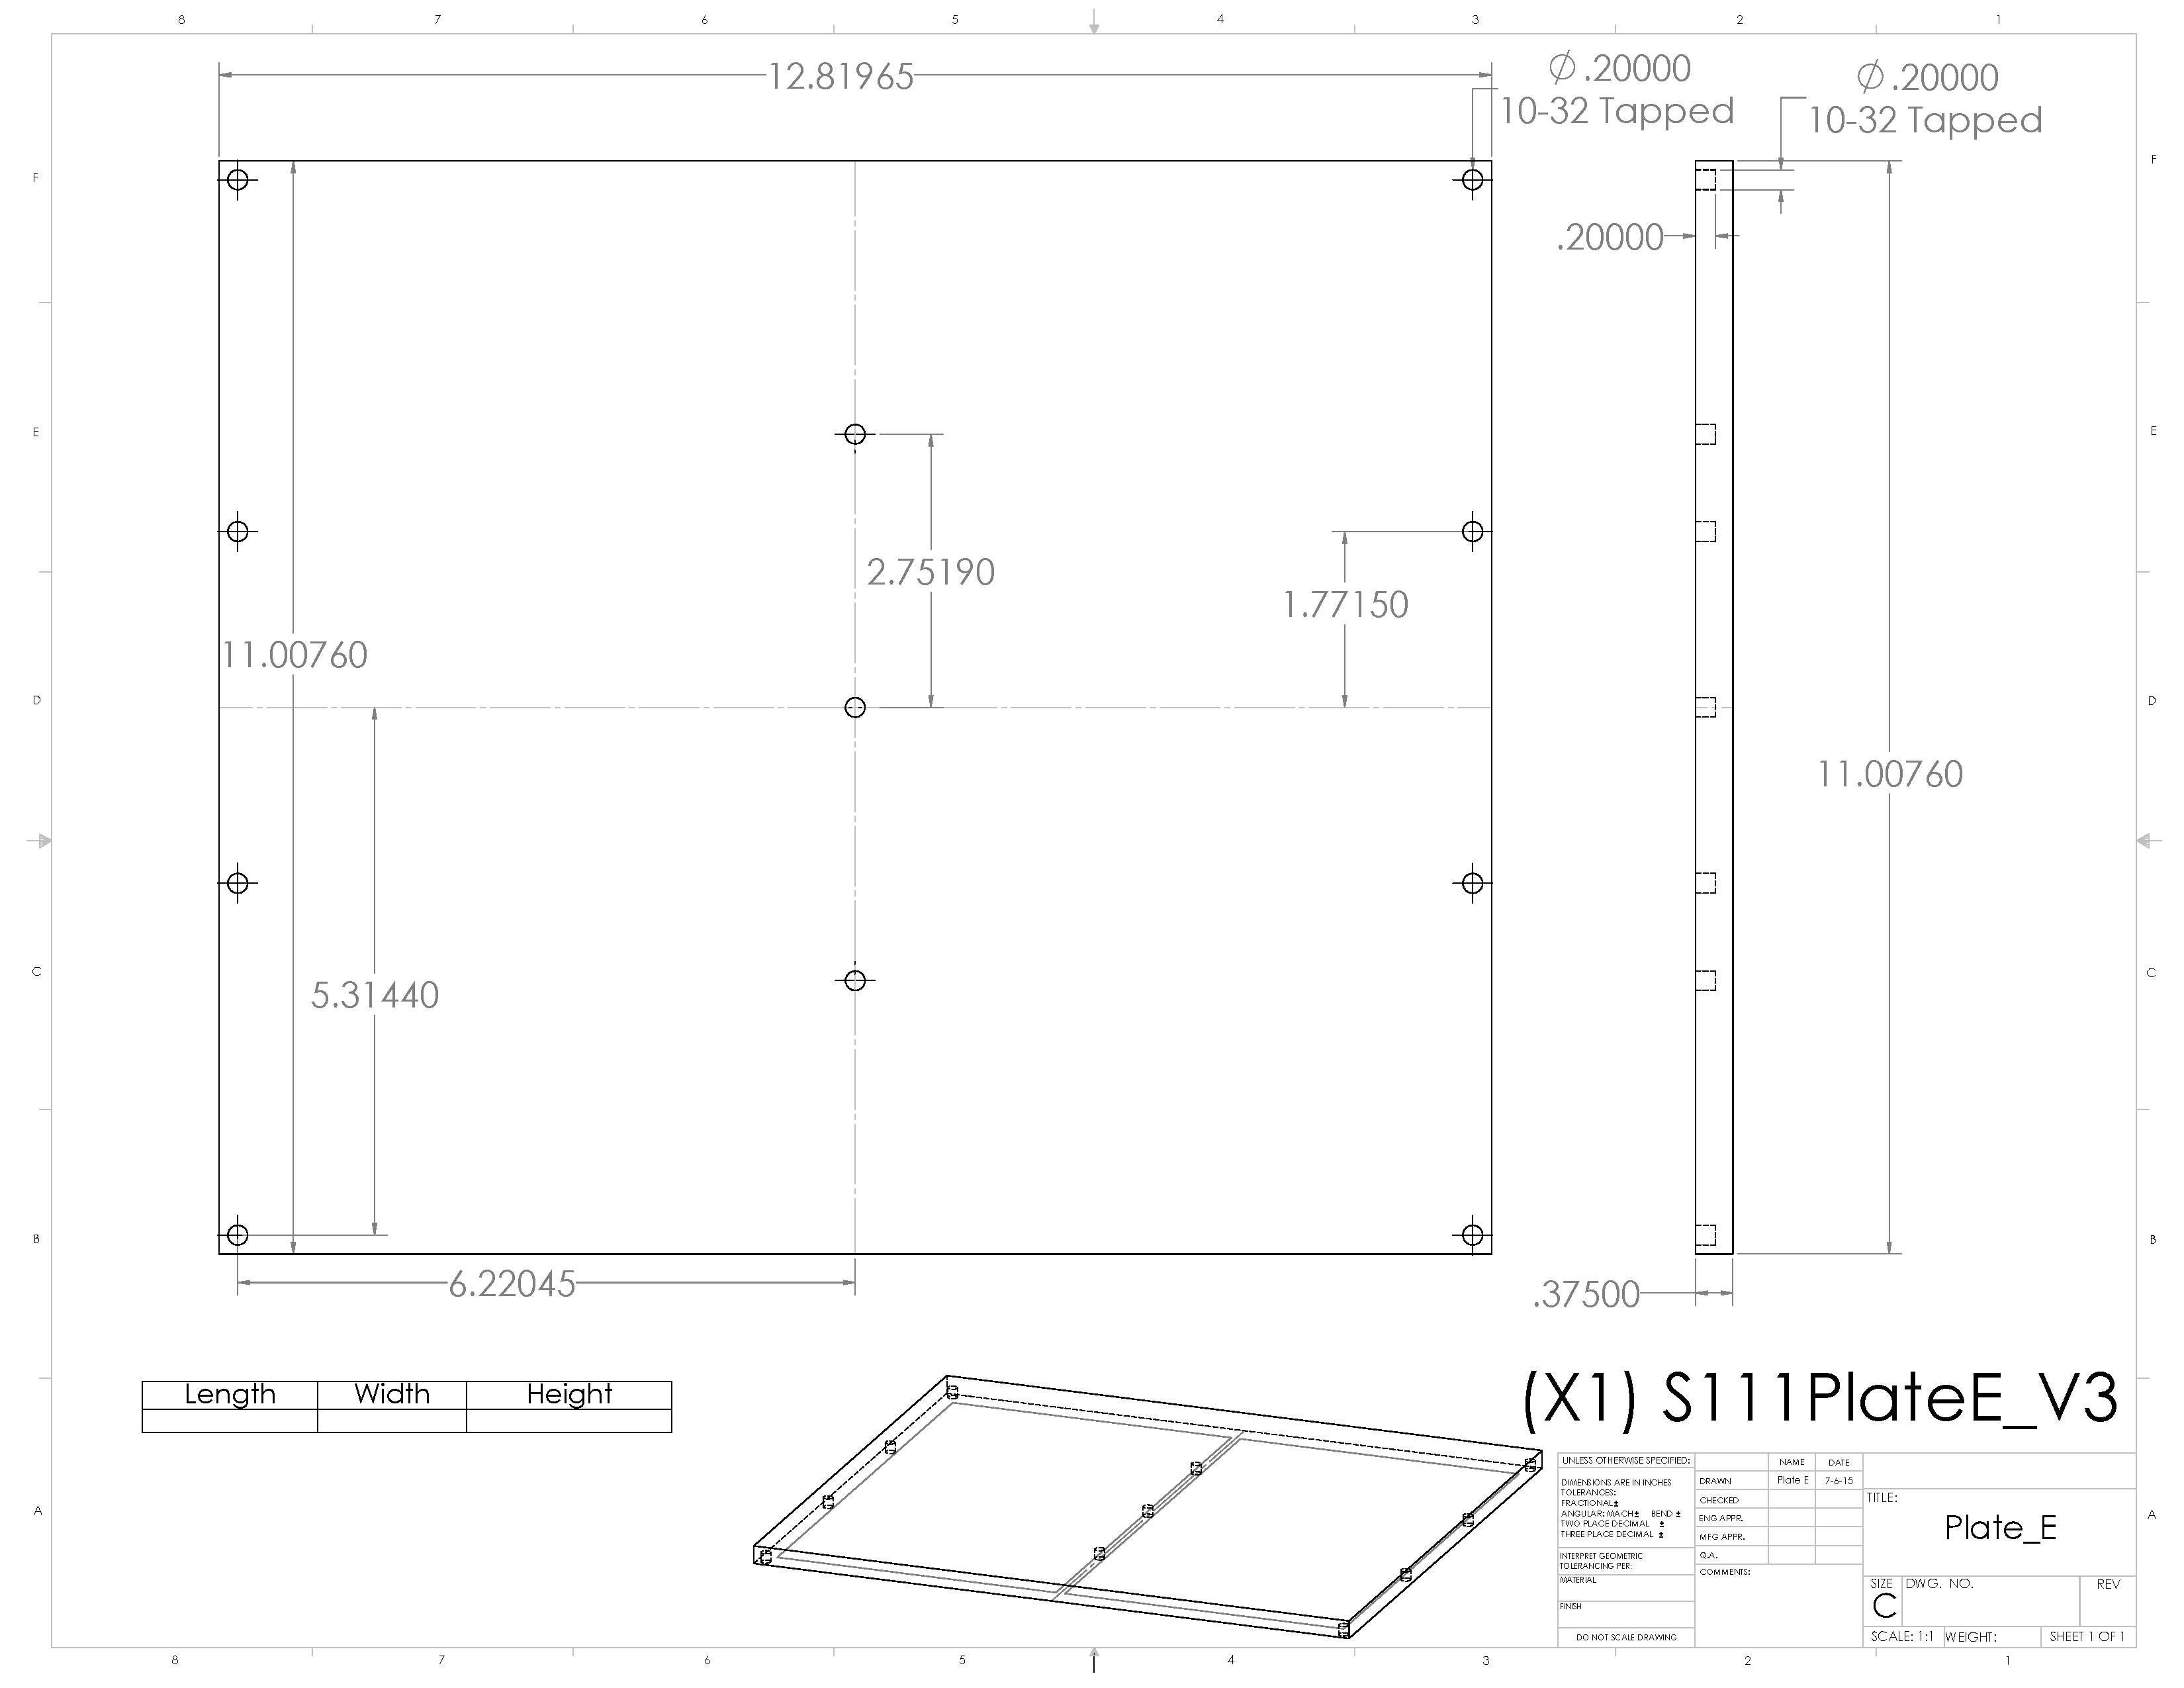
\includegraphics[scale=.2]{facility/drawings/Plate_E.PDF}
\caption{\footnotesize {\bf XX} } 
\end{figure}

\begin{figure}[h!]
  \begin{center}
  {\subfigcapskip = 5pt \subfigcapmargin = -12pt \subfigure[]{\label{fig:edge-a}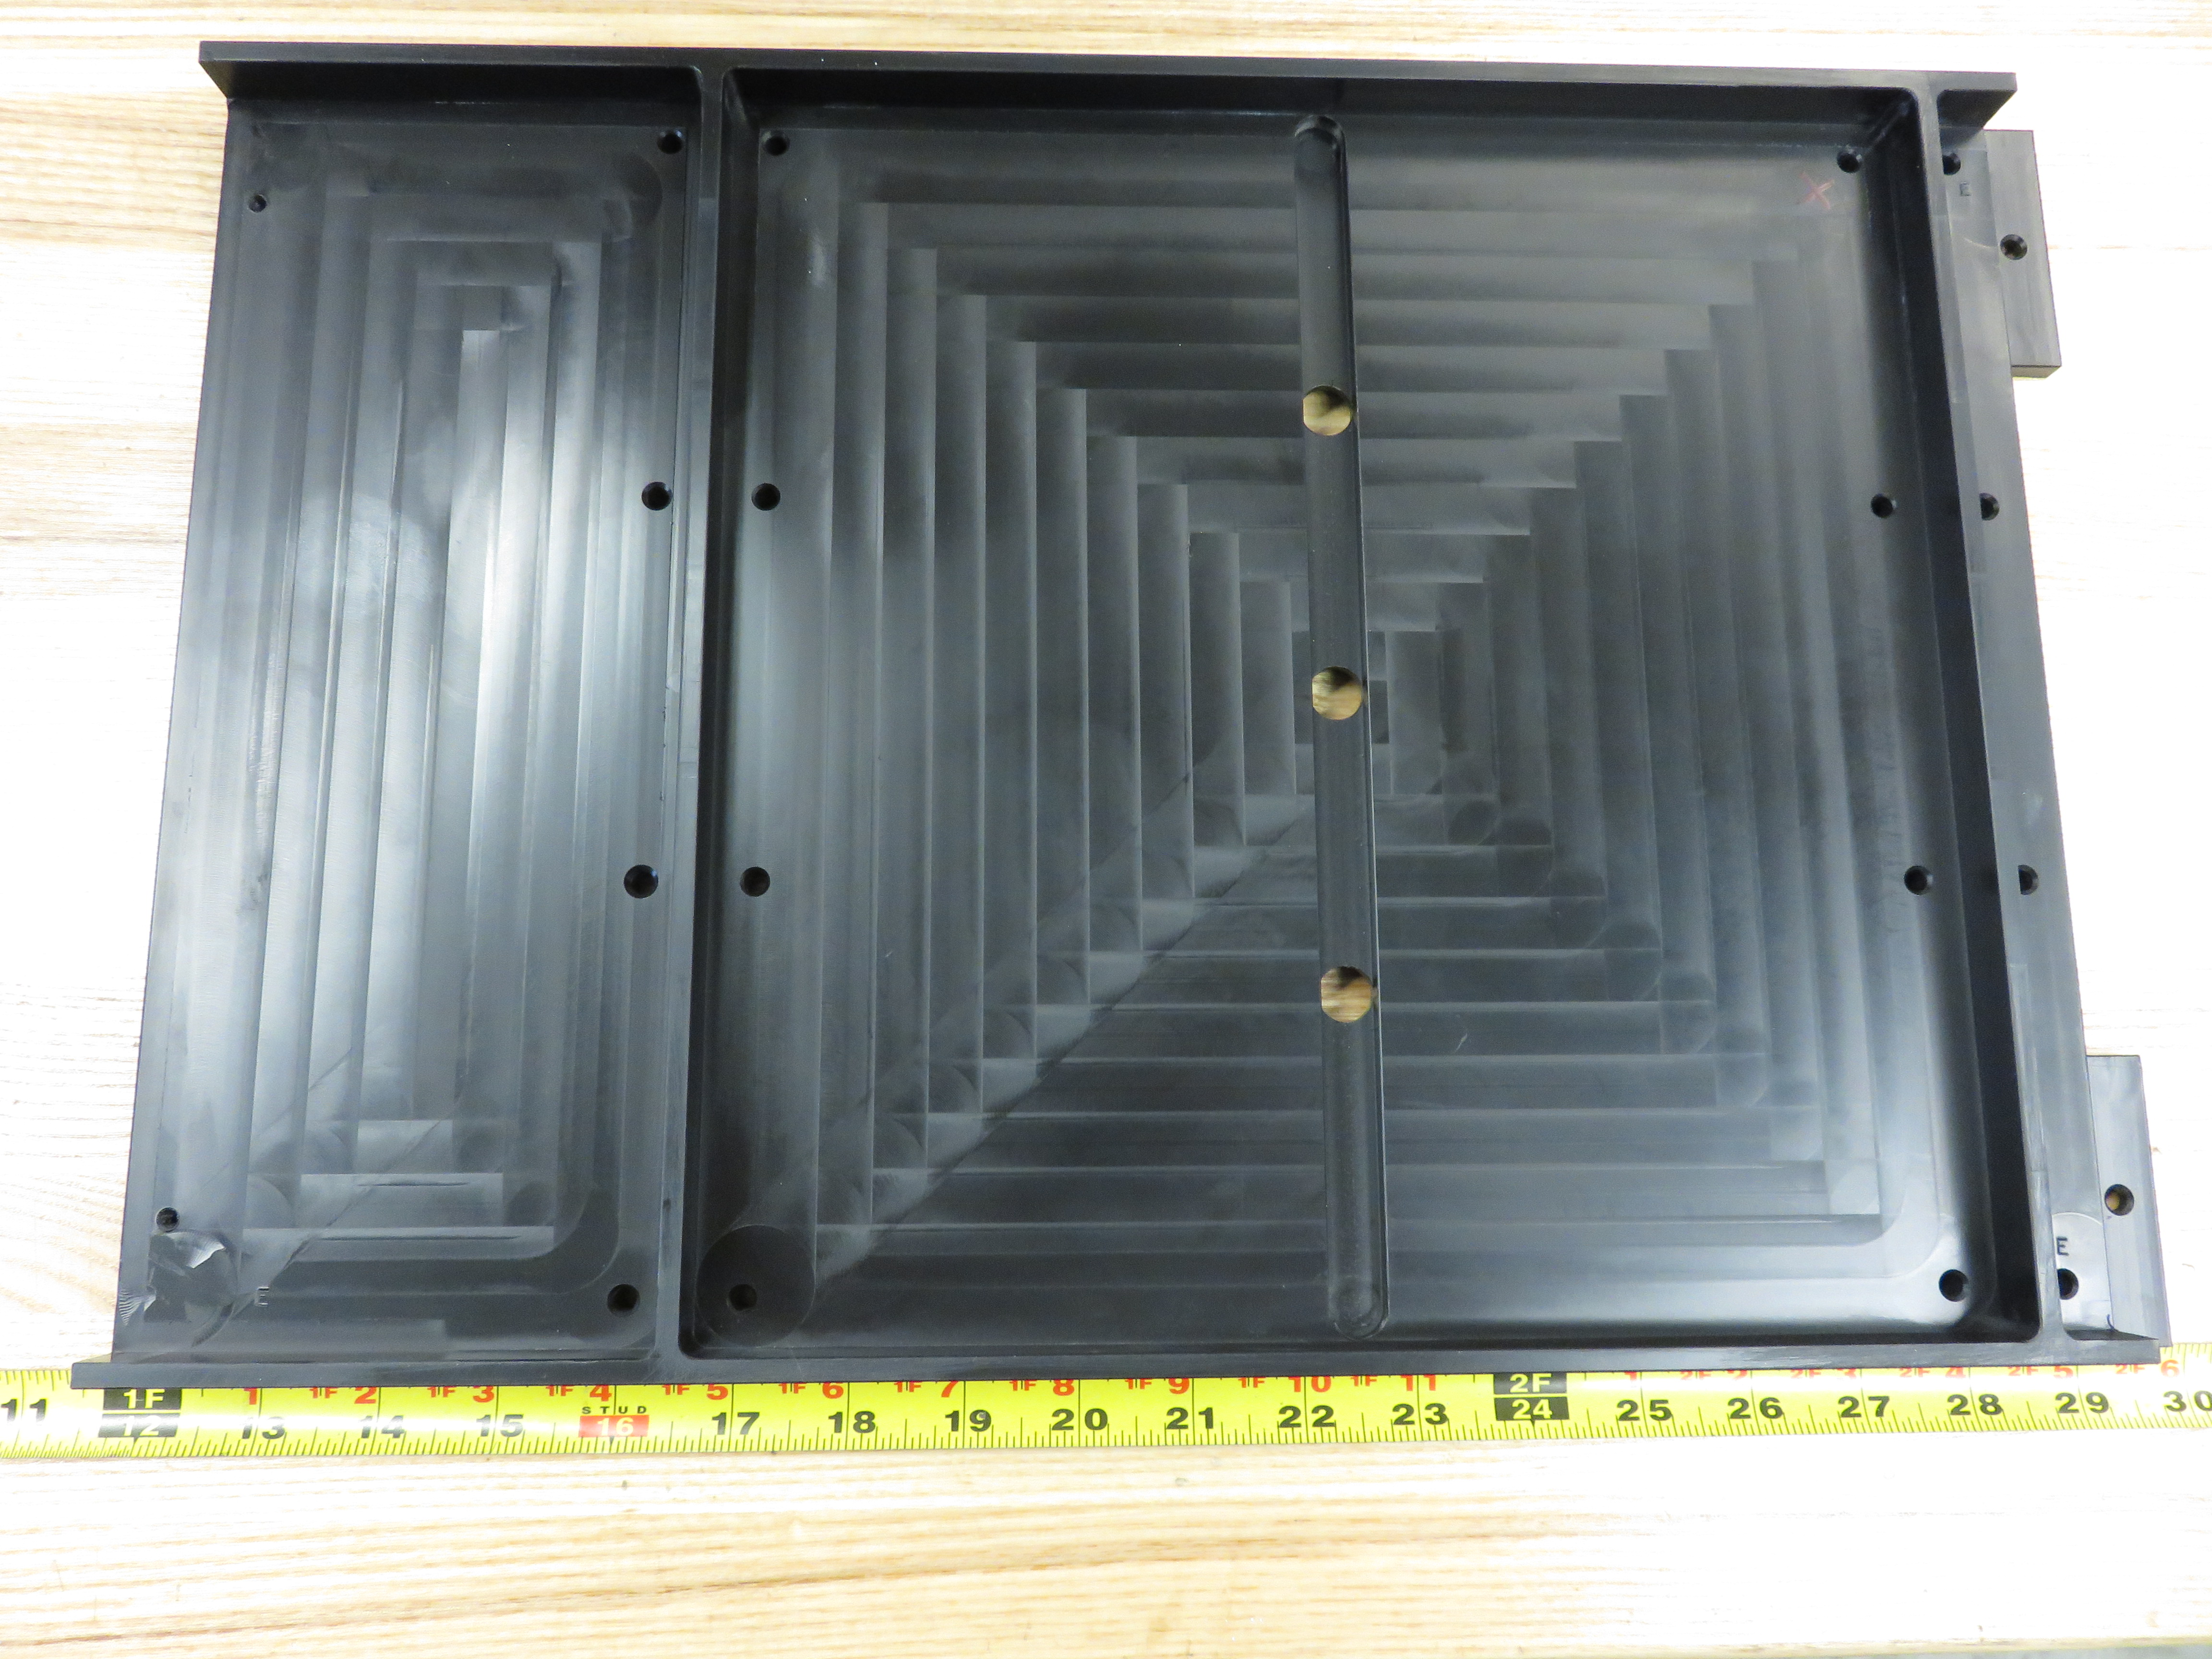
\includegraphics[scale=0.2]{facility/MachinedParts/E_meas_v2.JPG}}}
   {\subfigcapskip = 5pt \subfigcapmargin = -12pt  \subfigure[]{\label{fig:edge-b}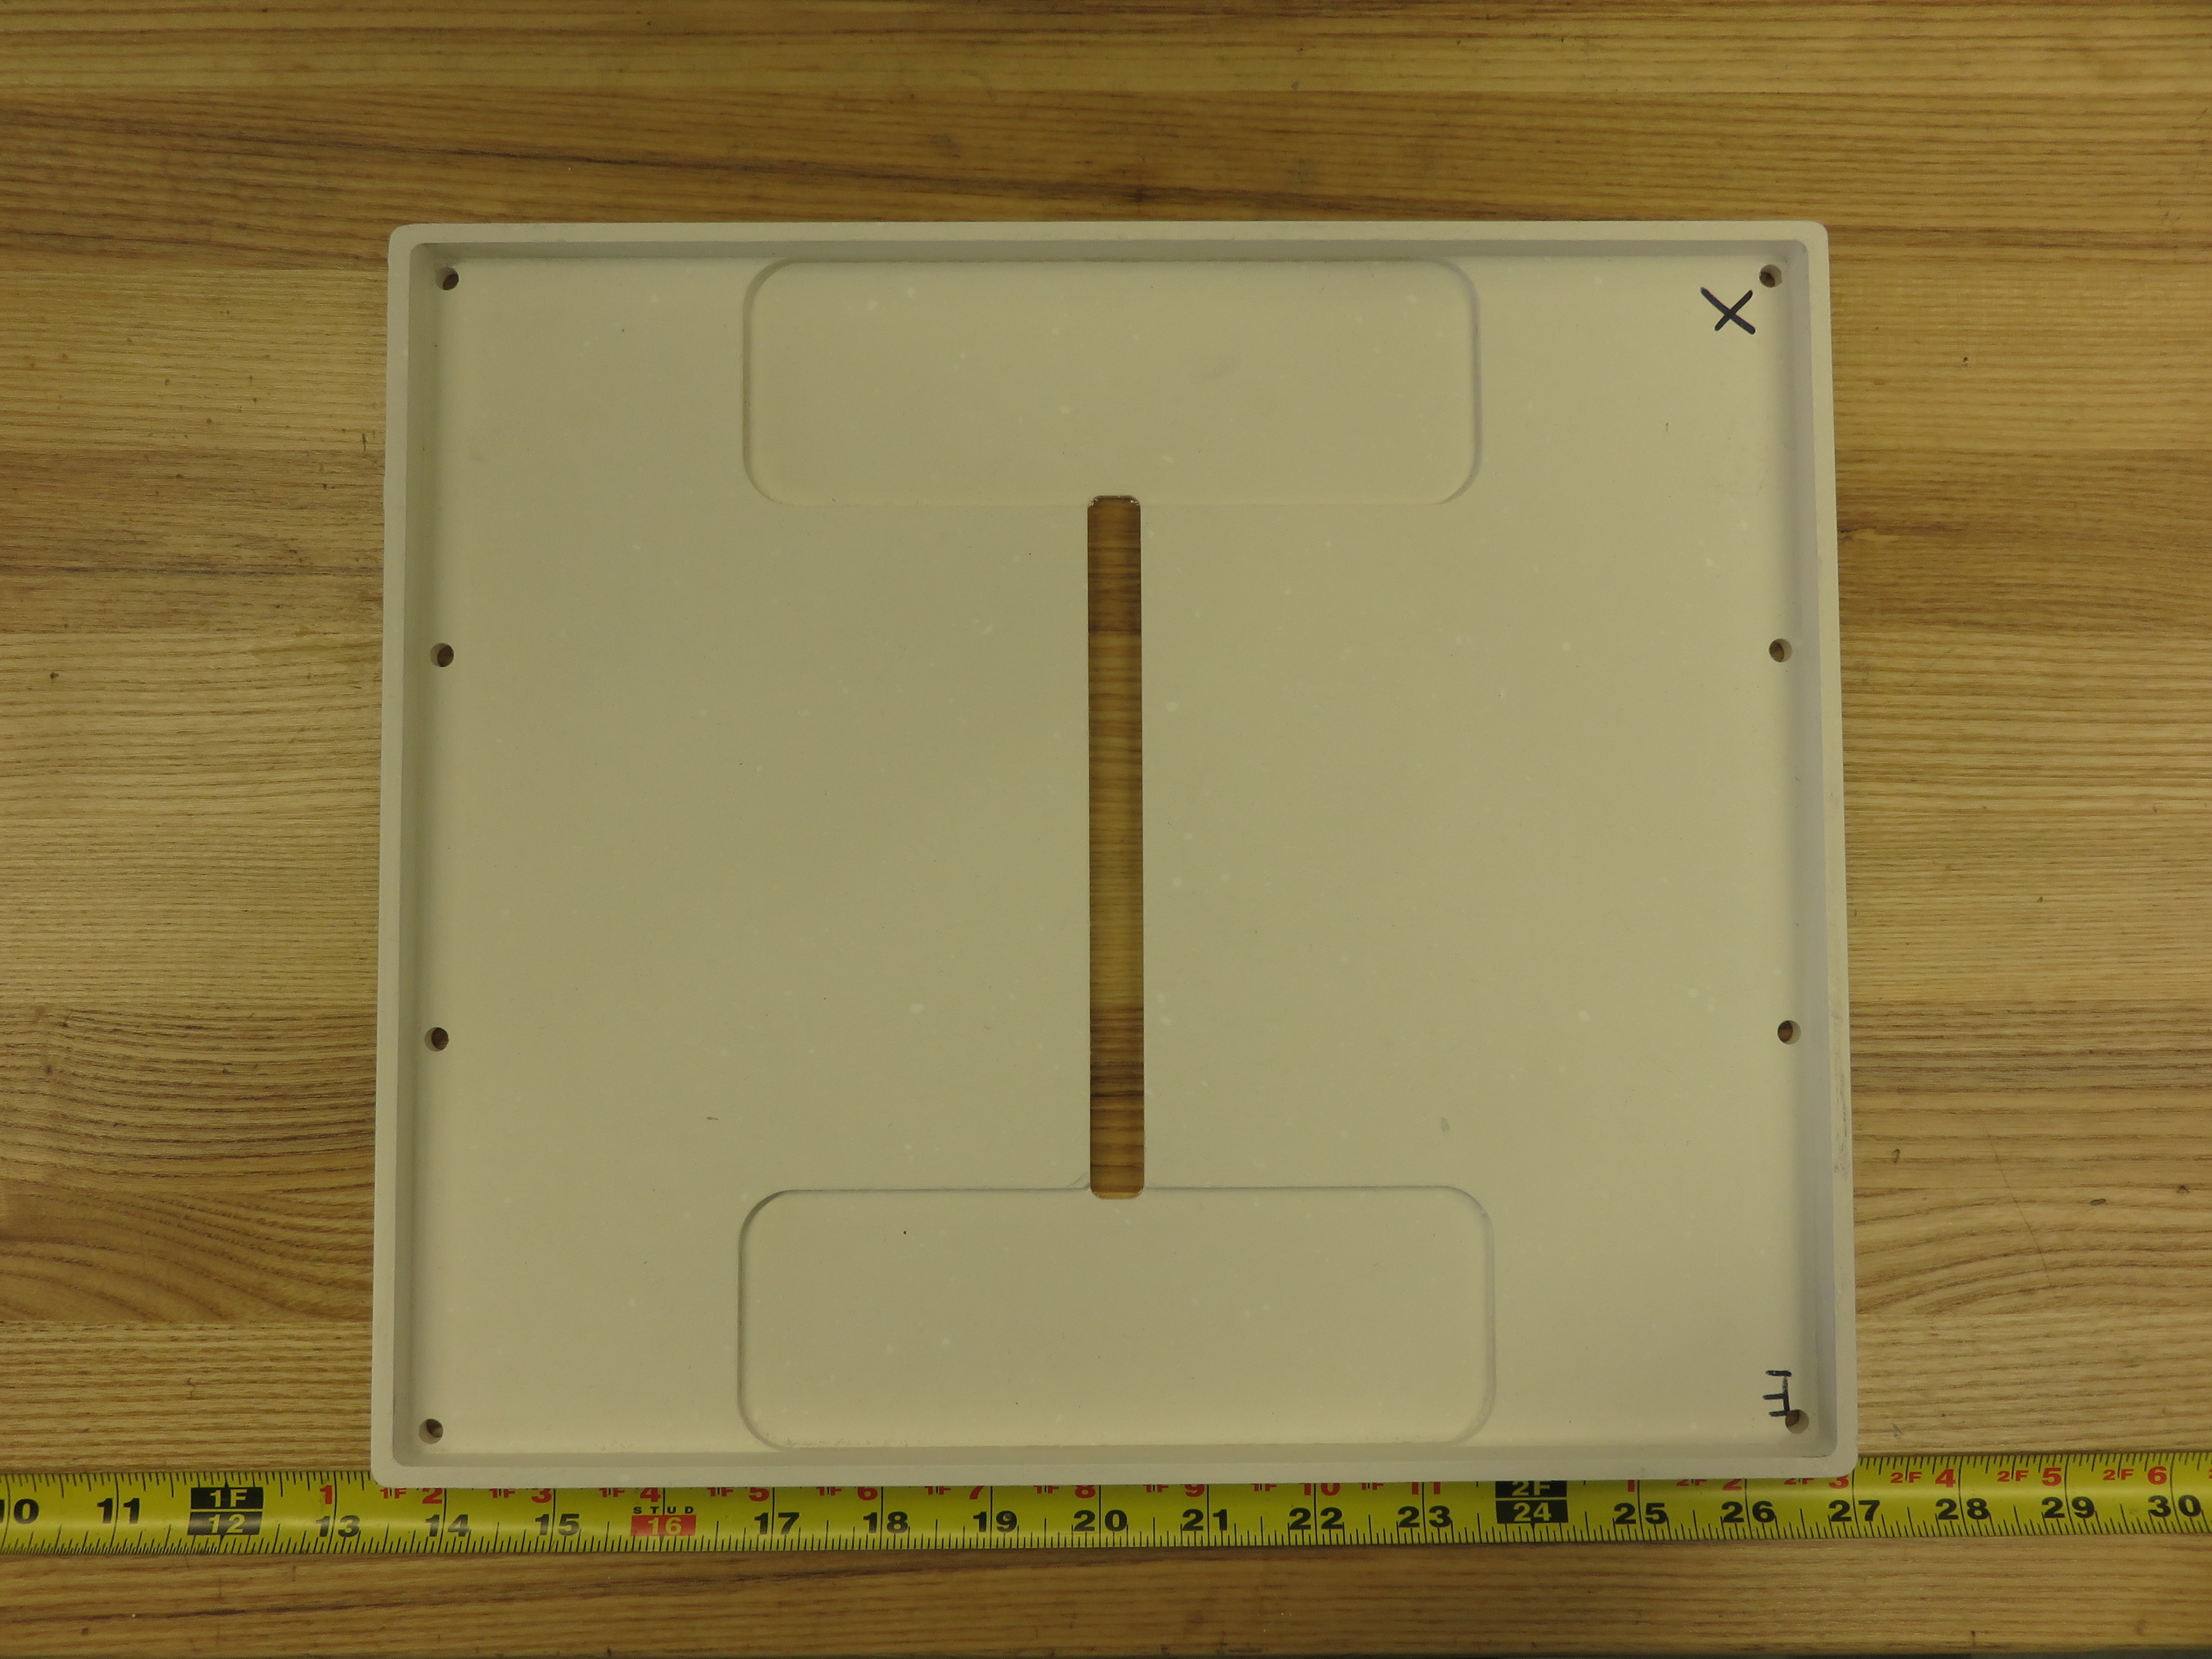
\includegraphics[scale=0.2]{facility/MachinedParts/E_insul_v2.JPG}}}
  \end{center}
\caption{(a) insulation (b) frame. } 
\end{figure}

%%%%%%%%%%%%%%%%%%%%%%%%%%%%%%%%%%%%%%%%%%%%%%%%%%%%%%
\clearpage
\subsection{Components F}
Input text description?\\

%components F
\begin{figure}[h!]
\centering
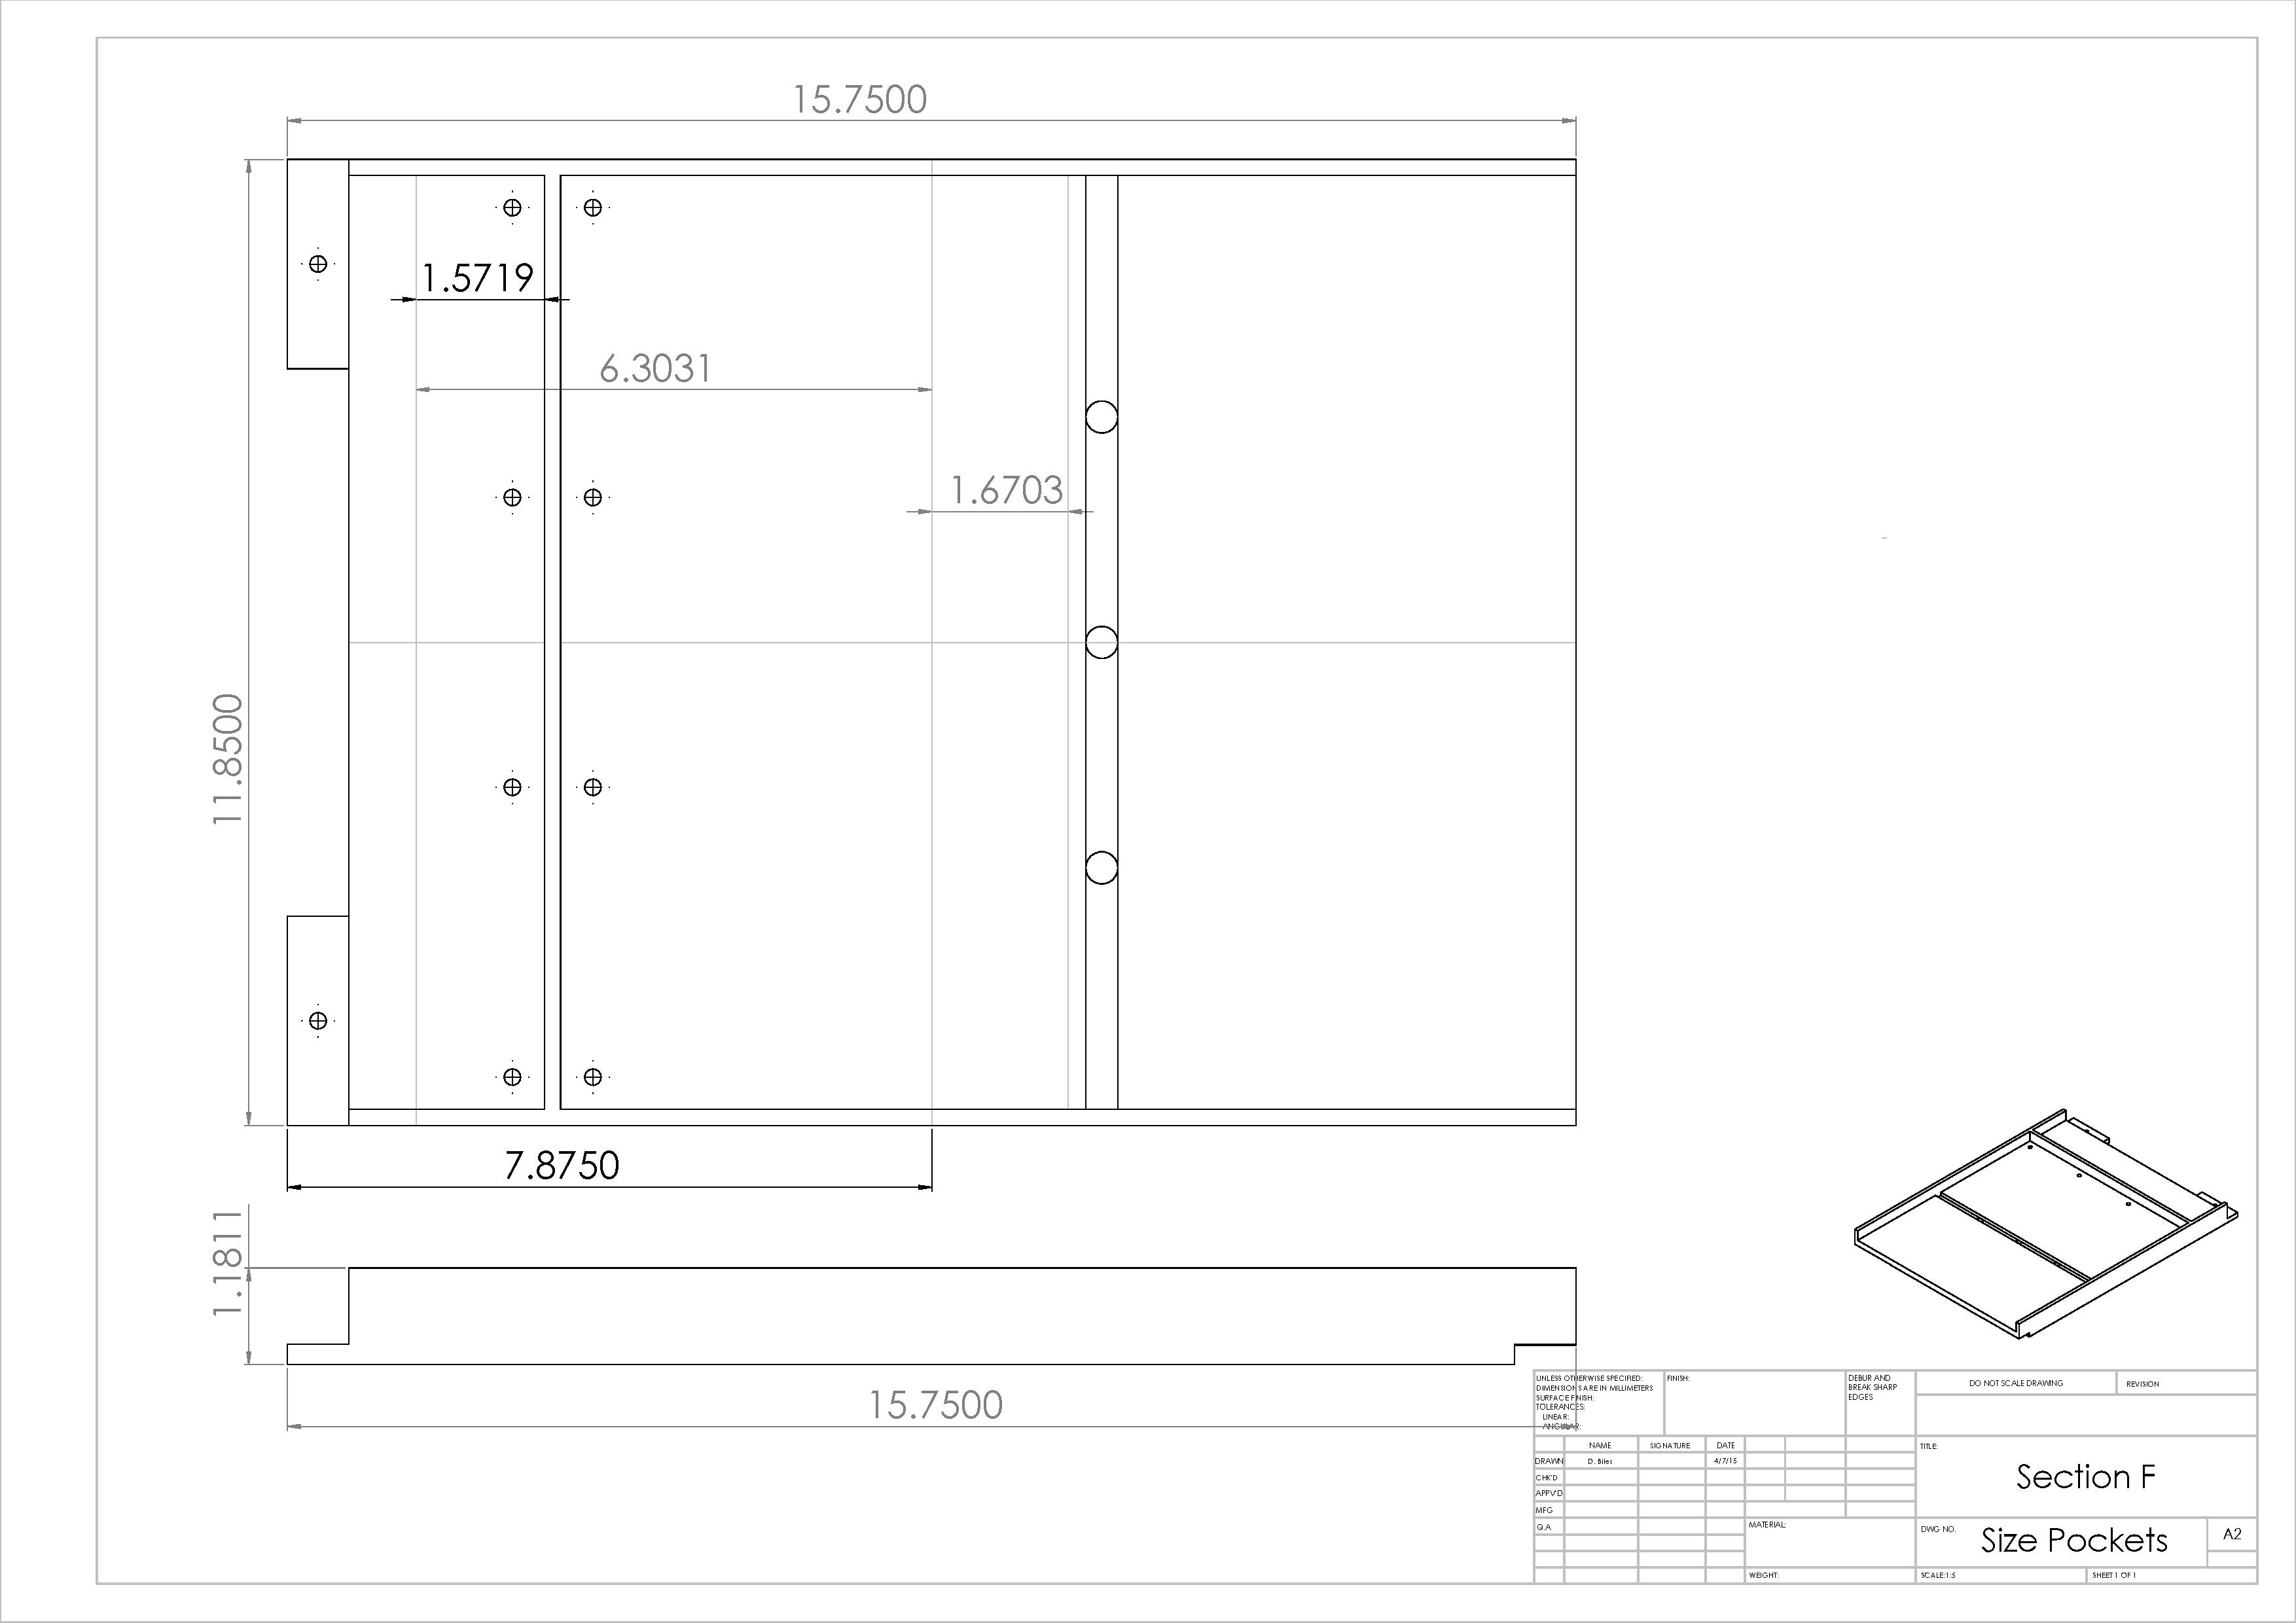
\includegraphics[scale=.2]{facility/drawings/F_size.PDF}
\caption{\footnotesize {\bf XX} } 
\end{figure}

\begin{figure}[h!]
\centering
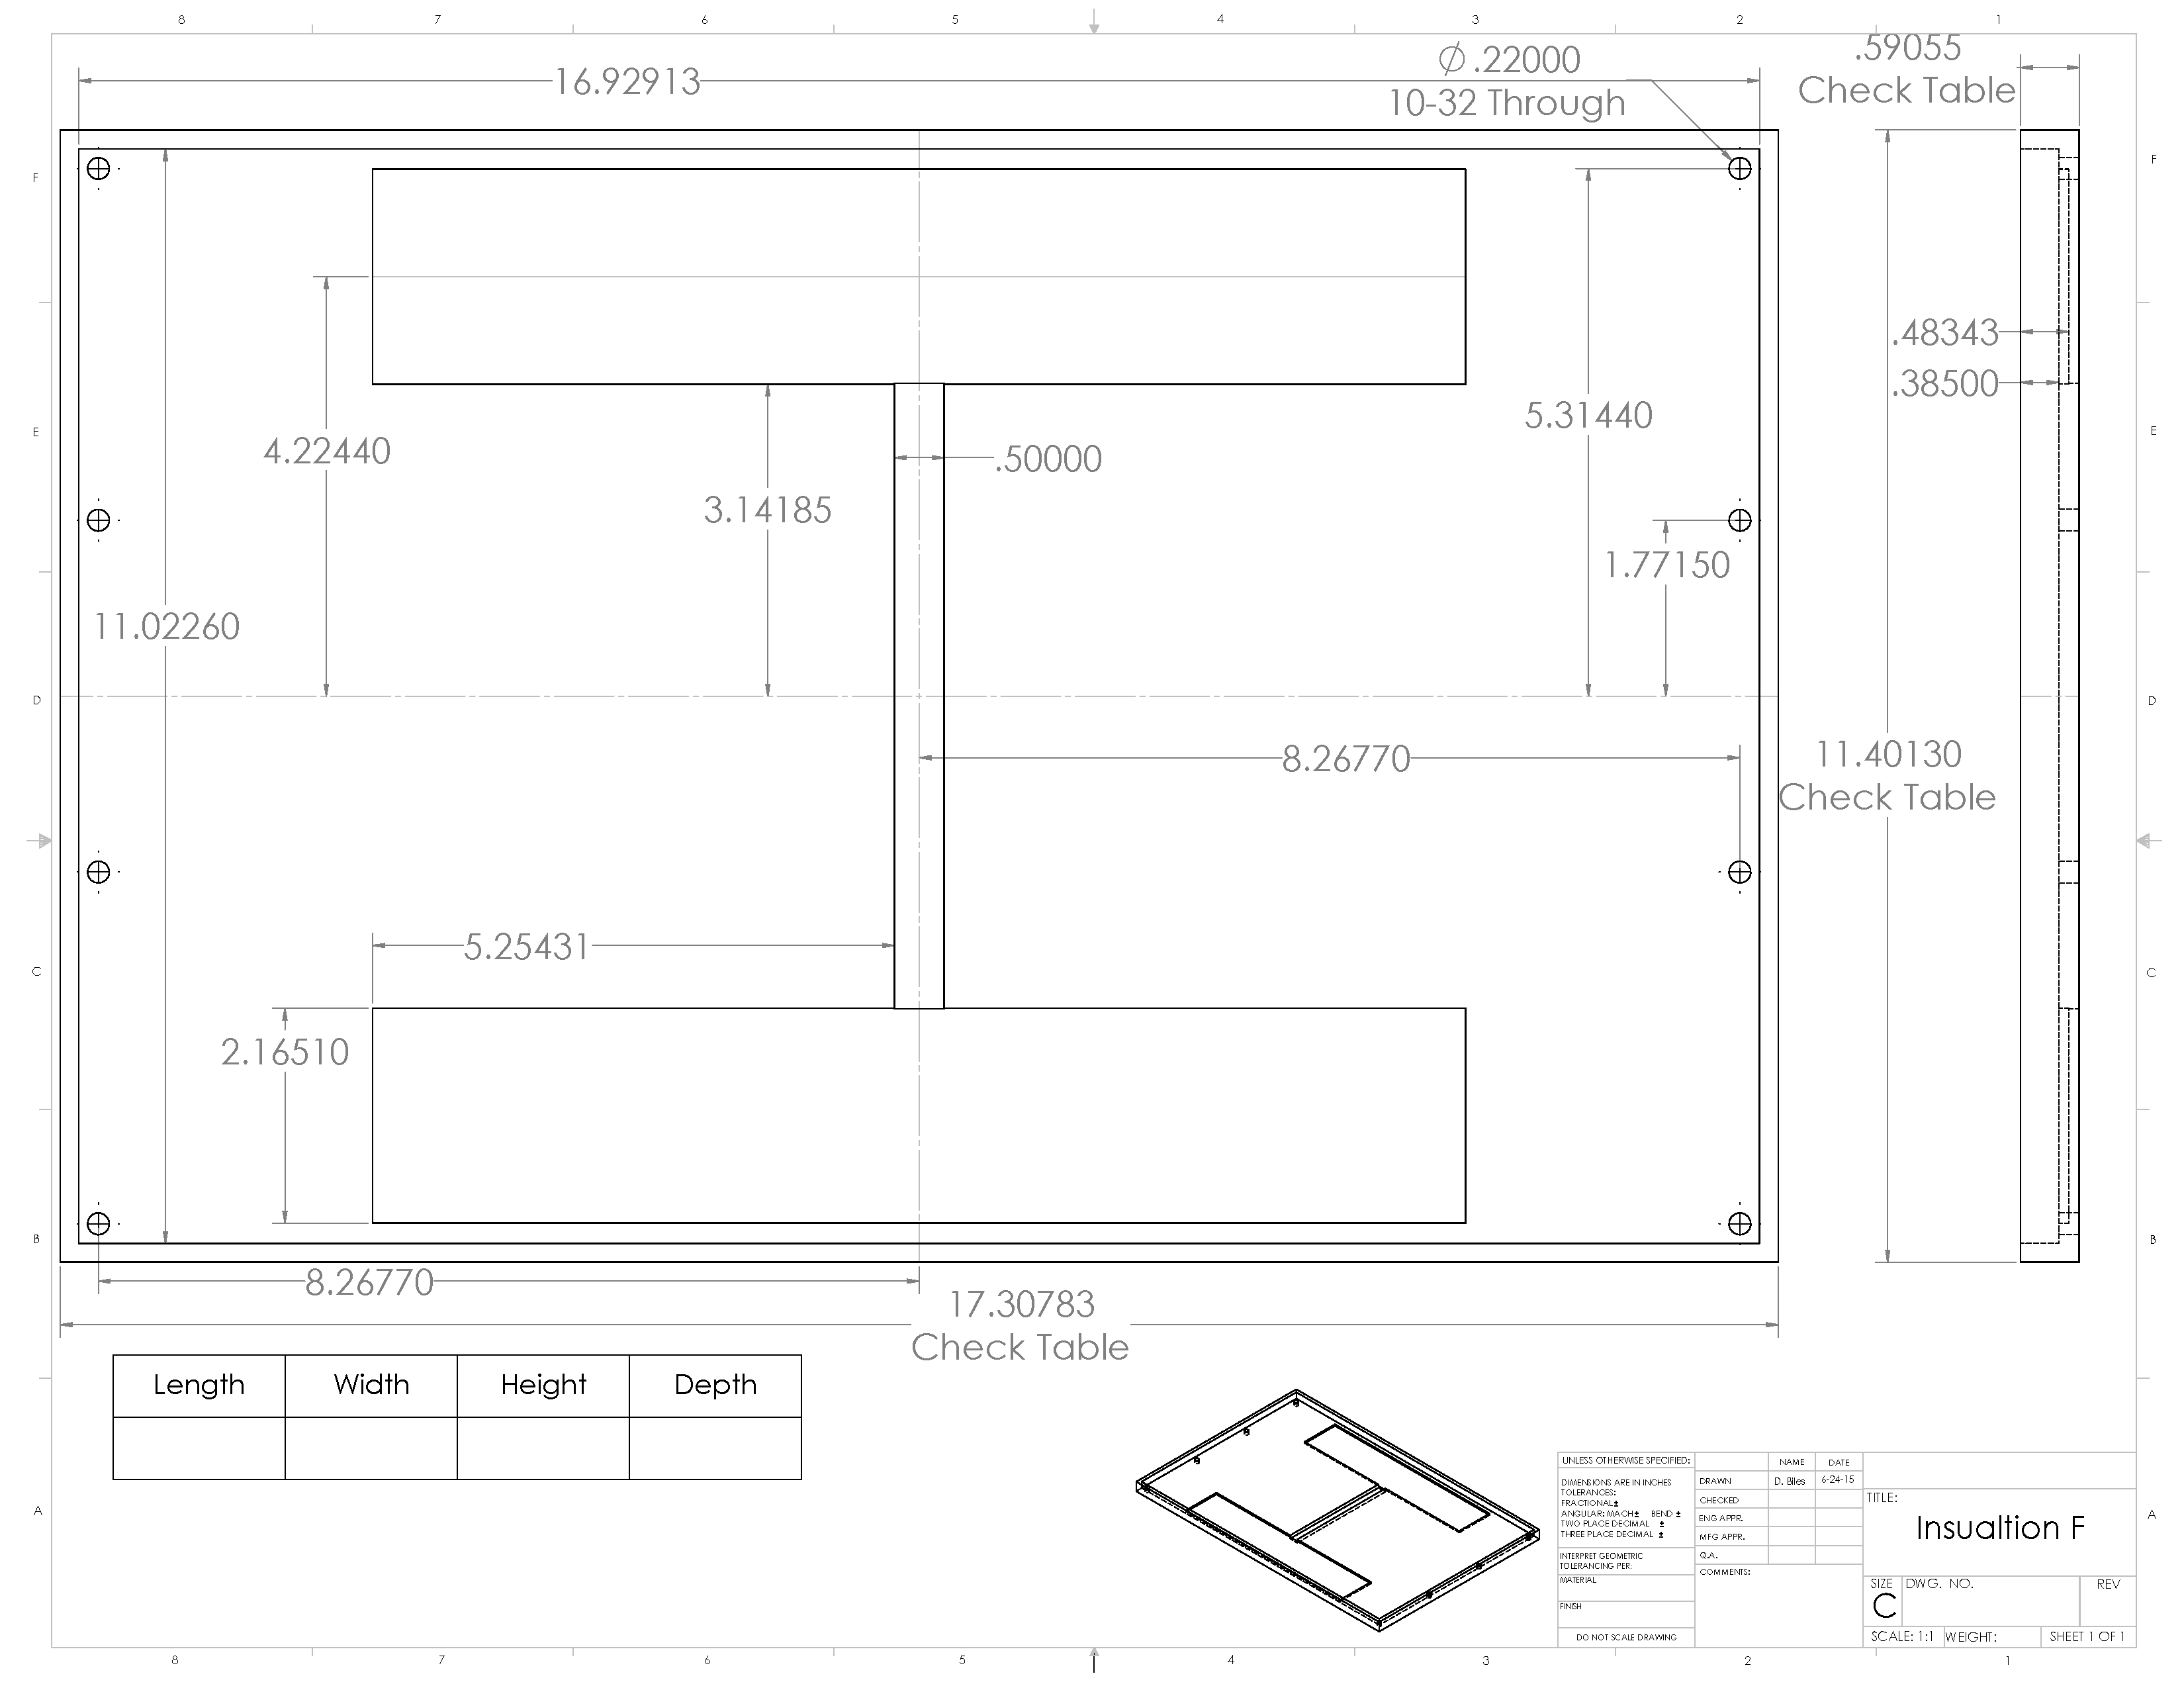
\includegraphics[scale=.2]{facility/drawings/Insulation_F.PDF}
\caption{\footnotesize {\bf XX} } 
\end{figure}

\begin{figure}[h!]
\centering
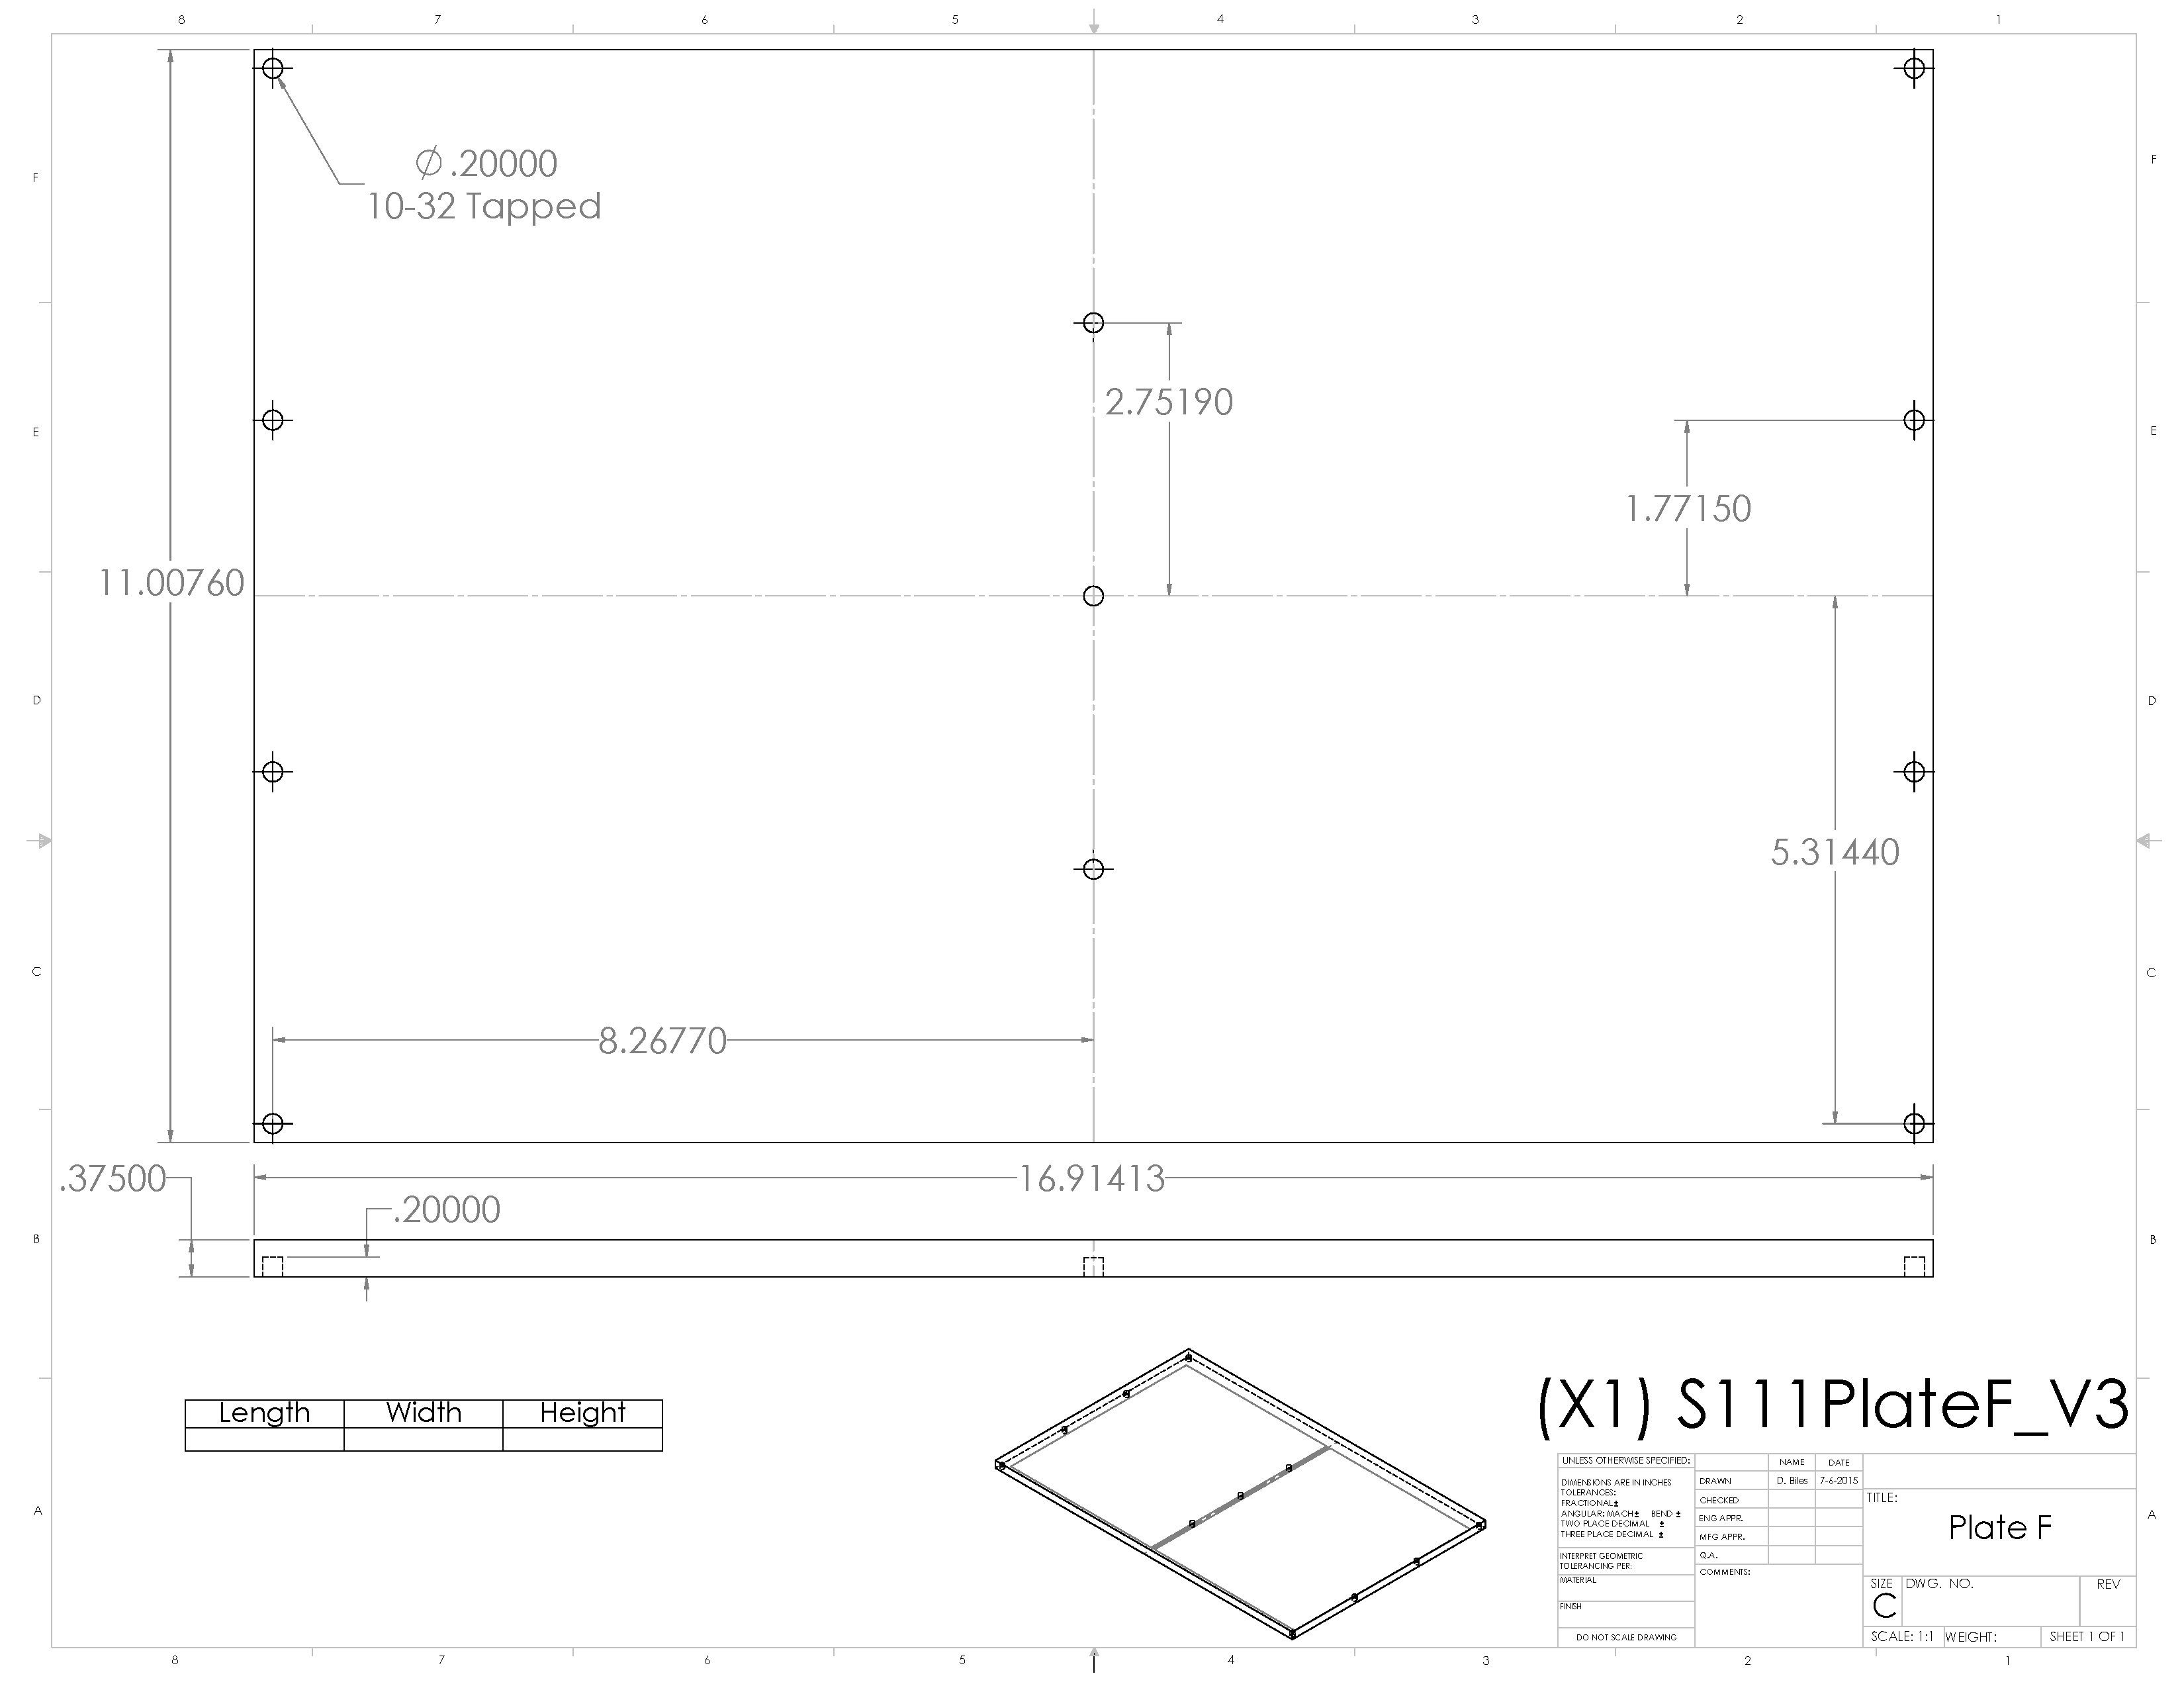
\includegraphics[scale=.2]{facility/drawings/Plate_F.PDF}
\caption{\footnotesize {\bf XX} } 
\end{figure}

\begin{figure}[h!]
  \begin{center}
  {\subfigcapskip = 5pt \subfigcapmargin = -12pt \subfigure[]{\label{fig:edge-a}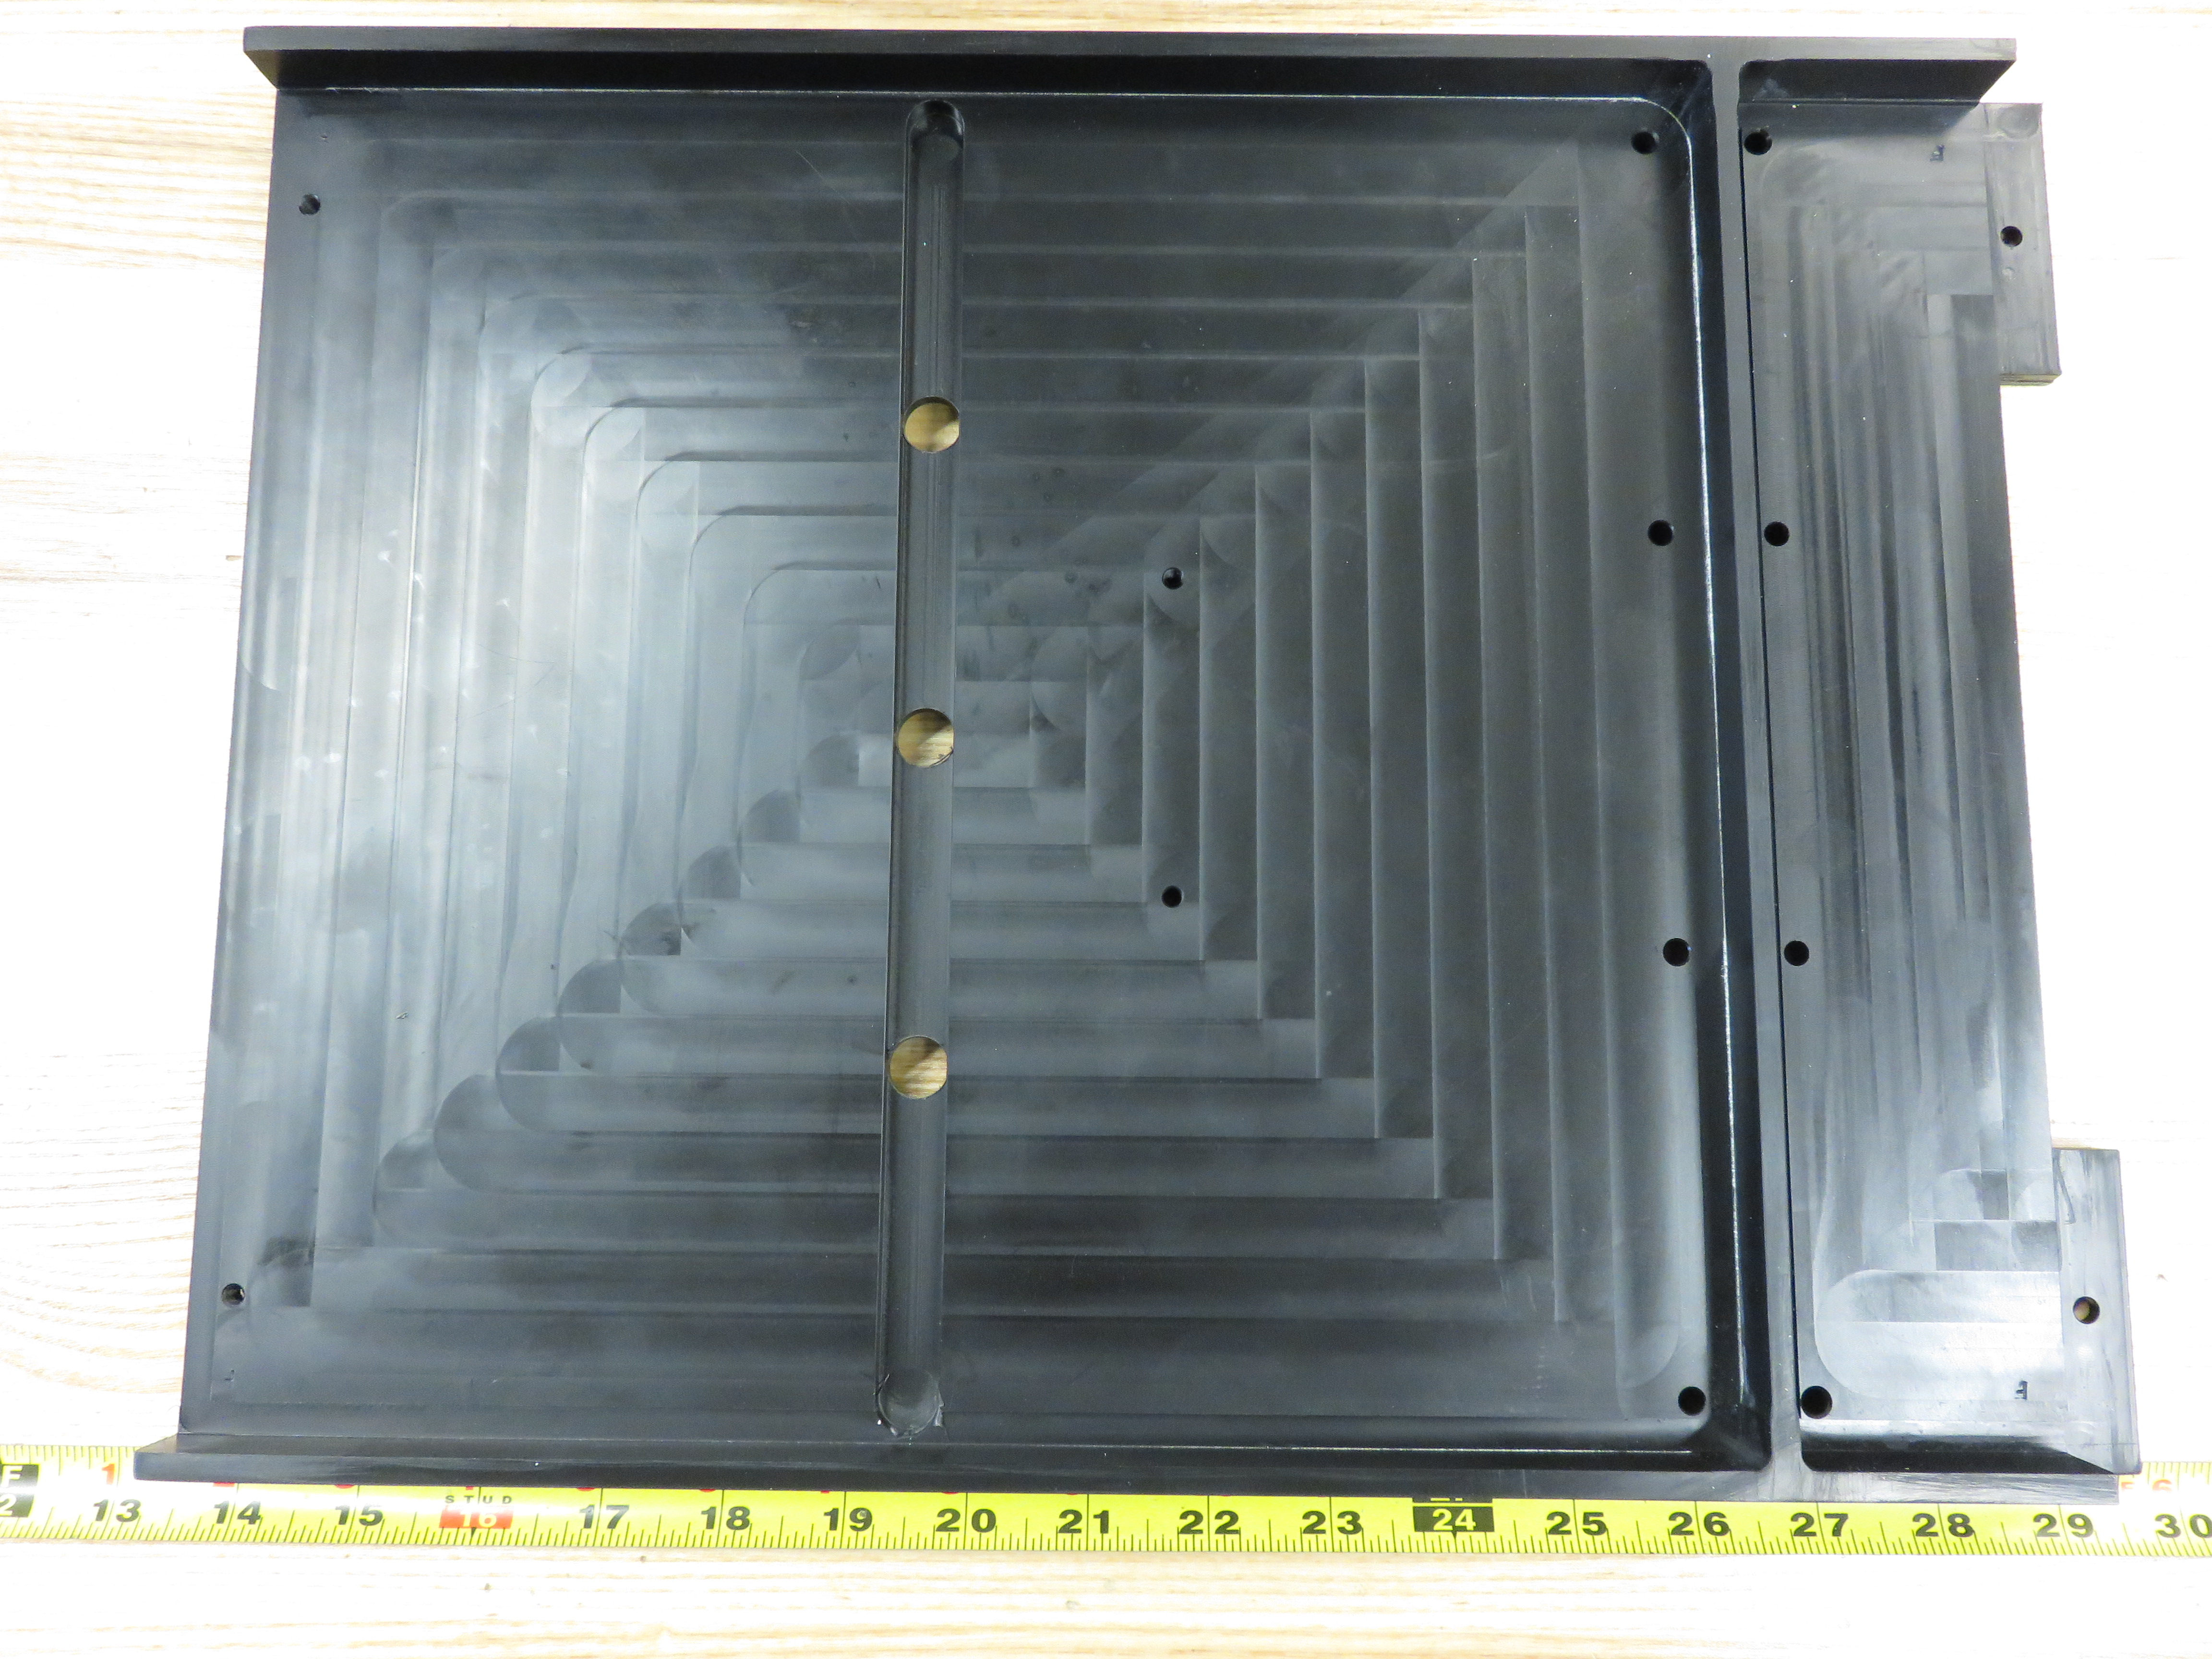
\includegraphics[scale=0.2]{facility/MachinedParts/F_meas_v1.JPG}}}
   {\subfigcapskip = 5pt \subfigcapmargin = -12pt  \subfigure[]{\label{fig:edge-b}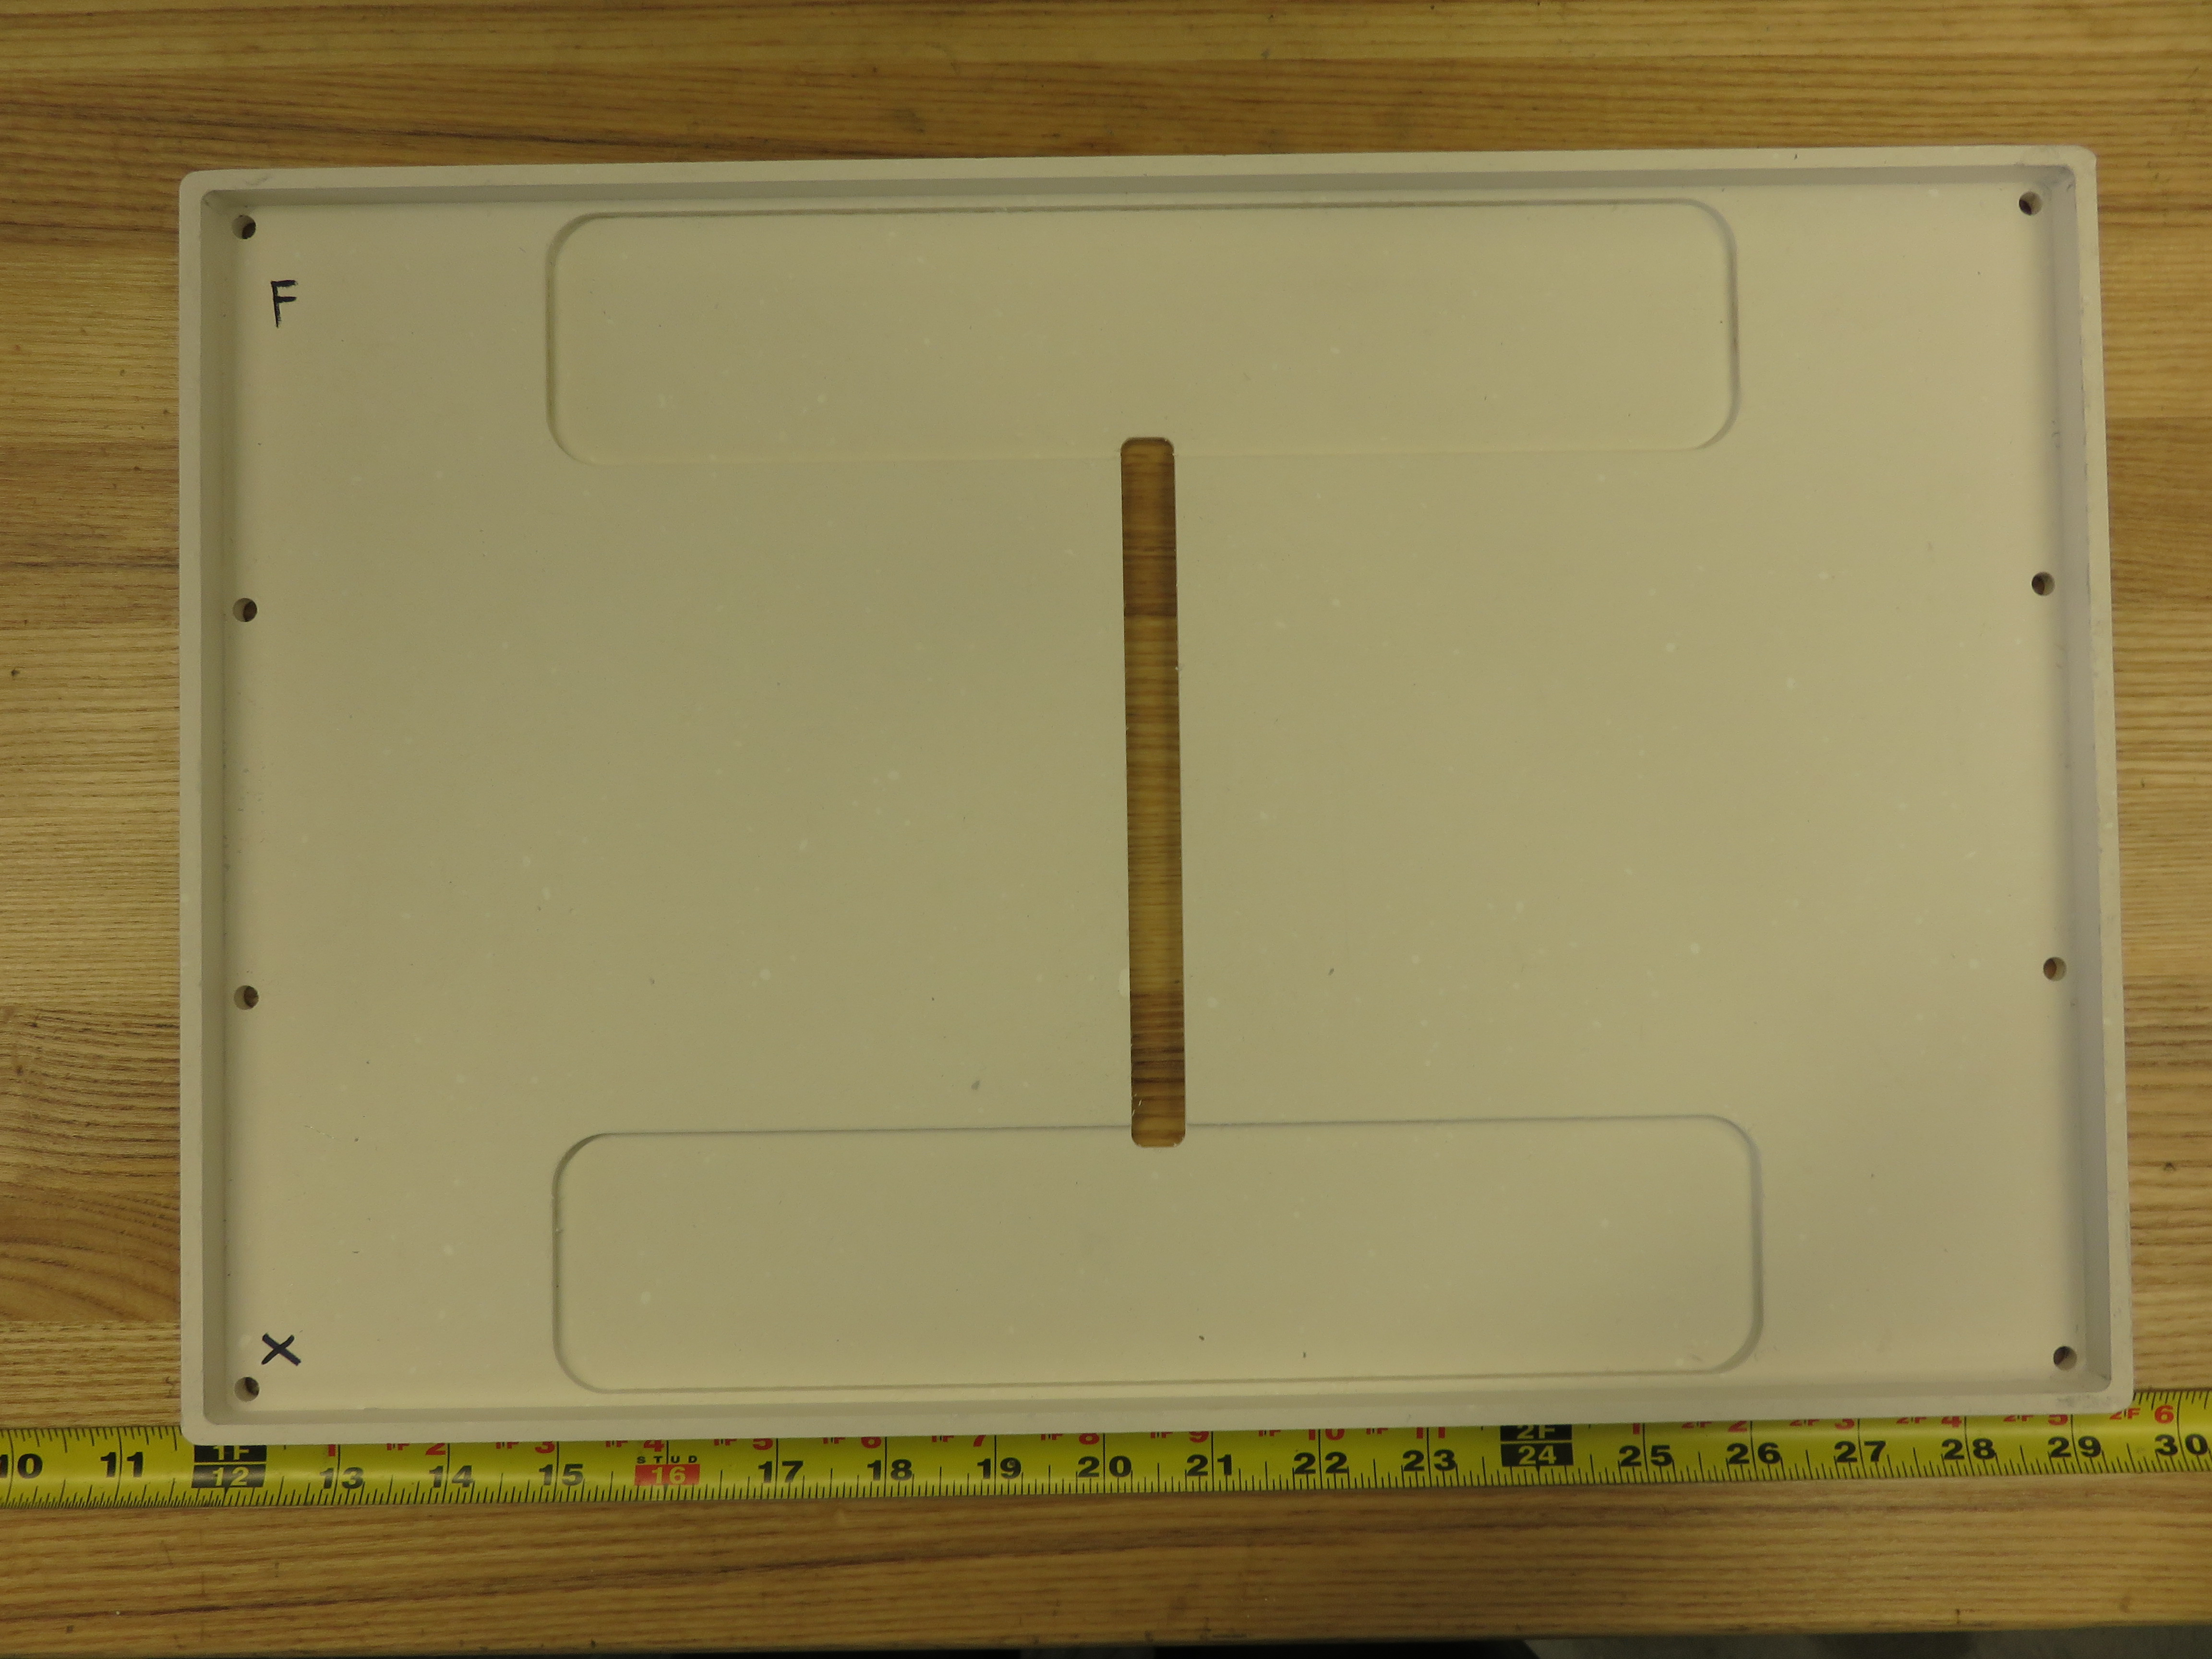
\includegraphics[scale=0.2]{facility/MachinedParts/F_insul_v2.JPG}}}
  \end{center}
\caption{(a) insulation (b) frame. } 
\end{figure}

%%%%%%%%%%%%%%%%%%%%%%%%%%%%%%%%%%%%%%%%%%%%%%%%%%%%%%
\clearpage
\subsection{Components G}
Input text description?\\

\begin{figure}[h!]
\centering
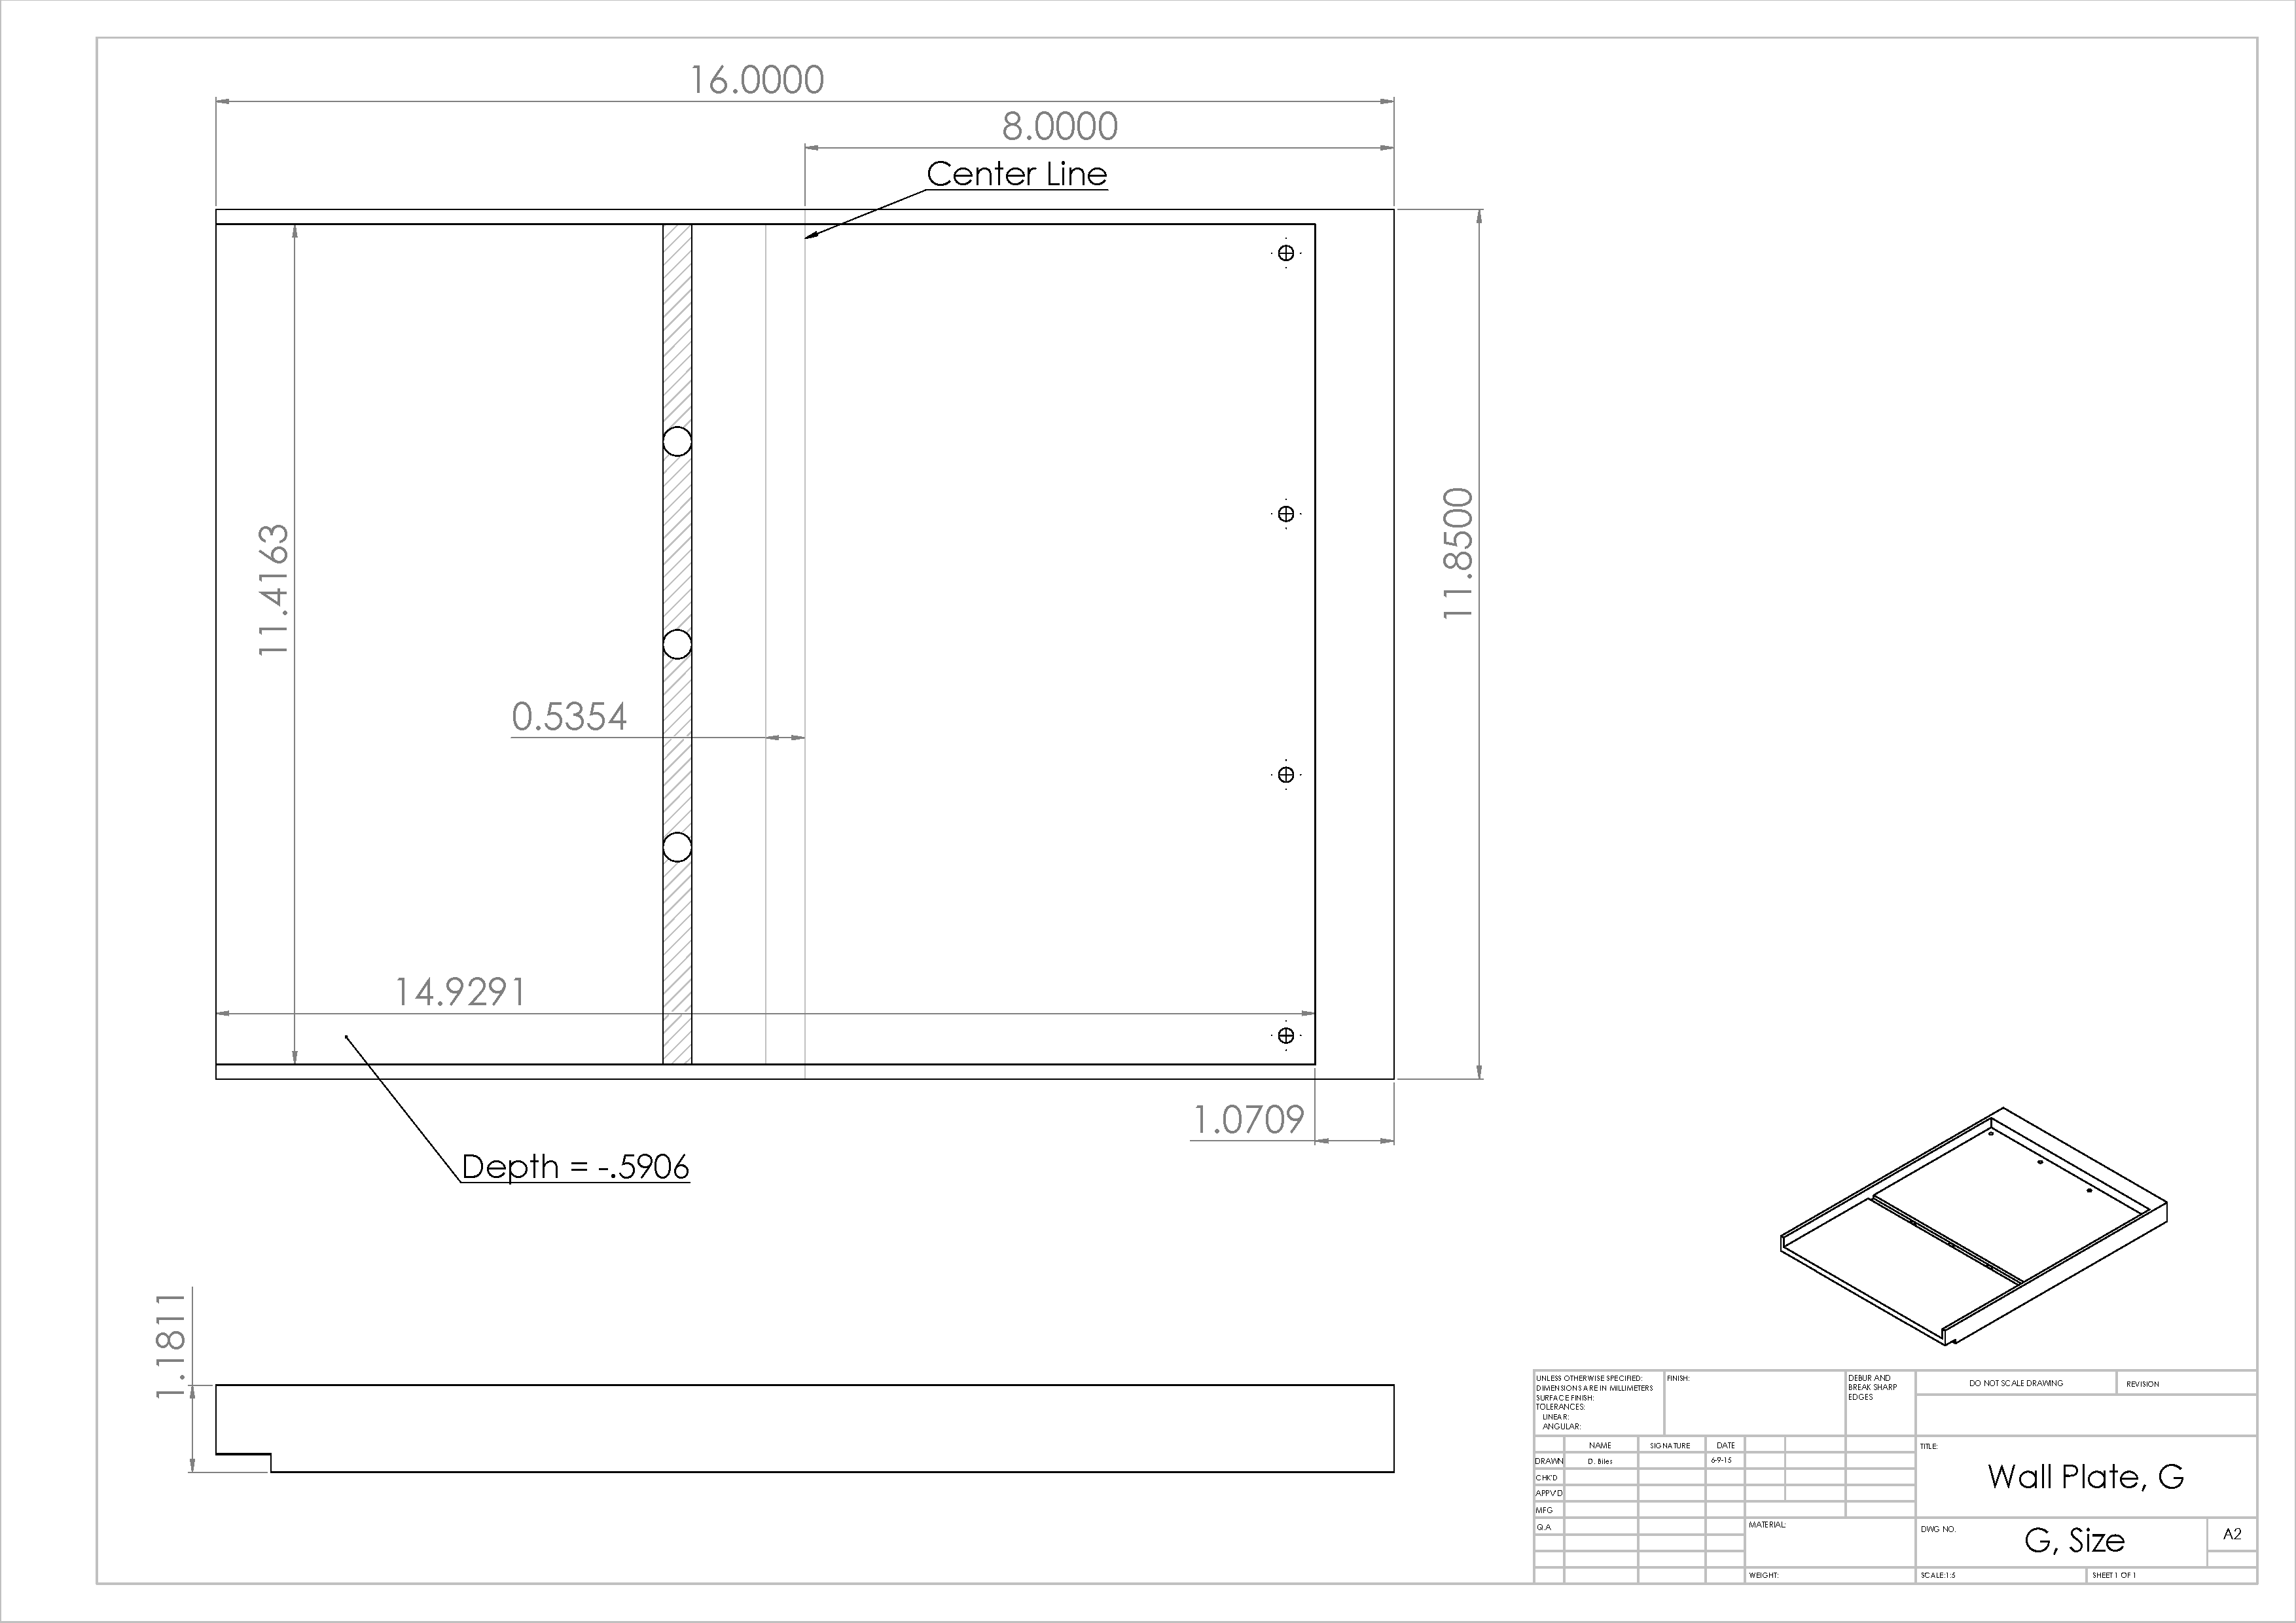
\includegraphics[scale=.18]{facility/drawings/G_size.PDF}
\caption{\footnotesize {\bf XX} } 
\end{figure}


\begin{figure}[h!]
\centering
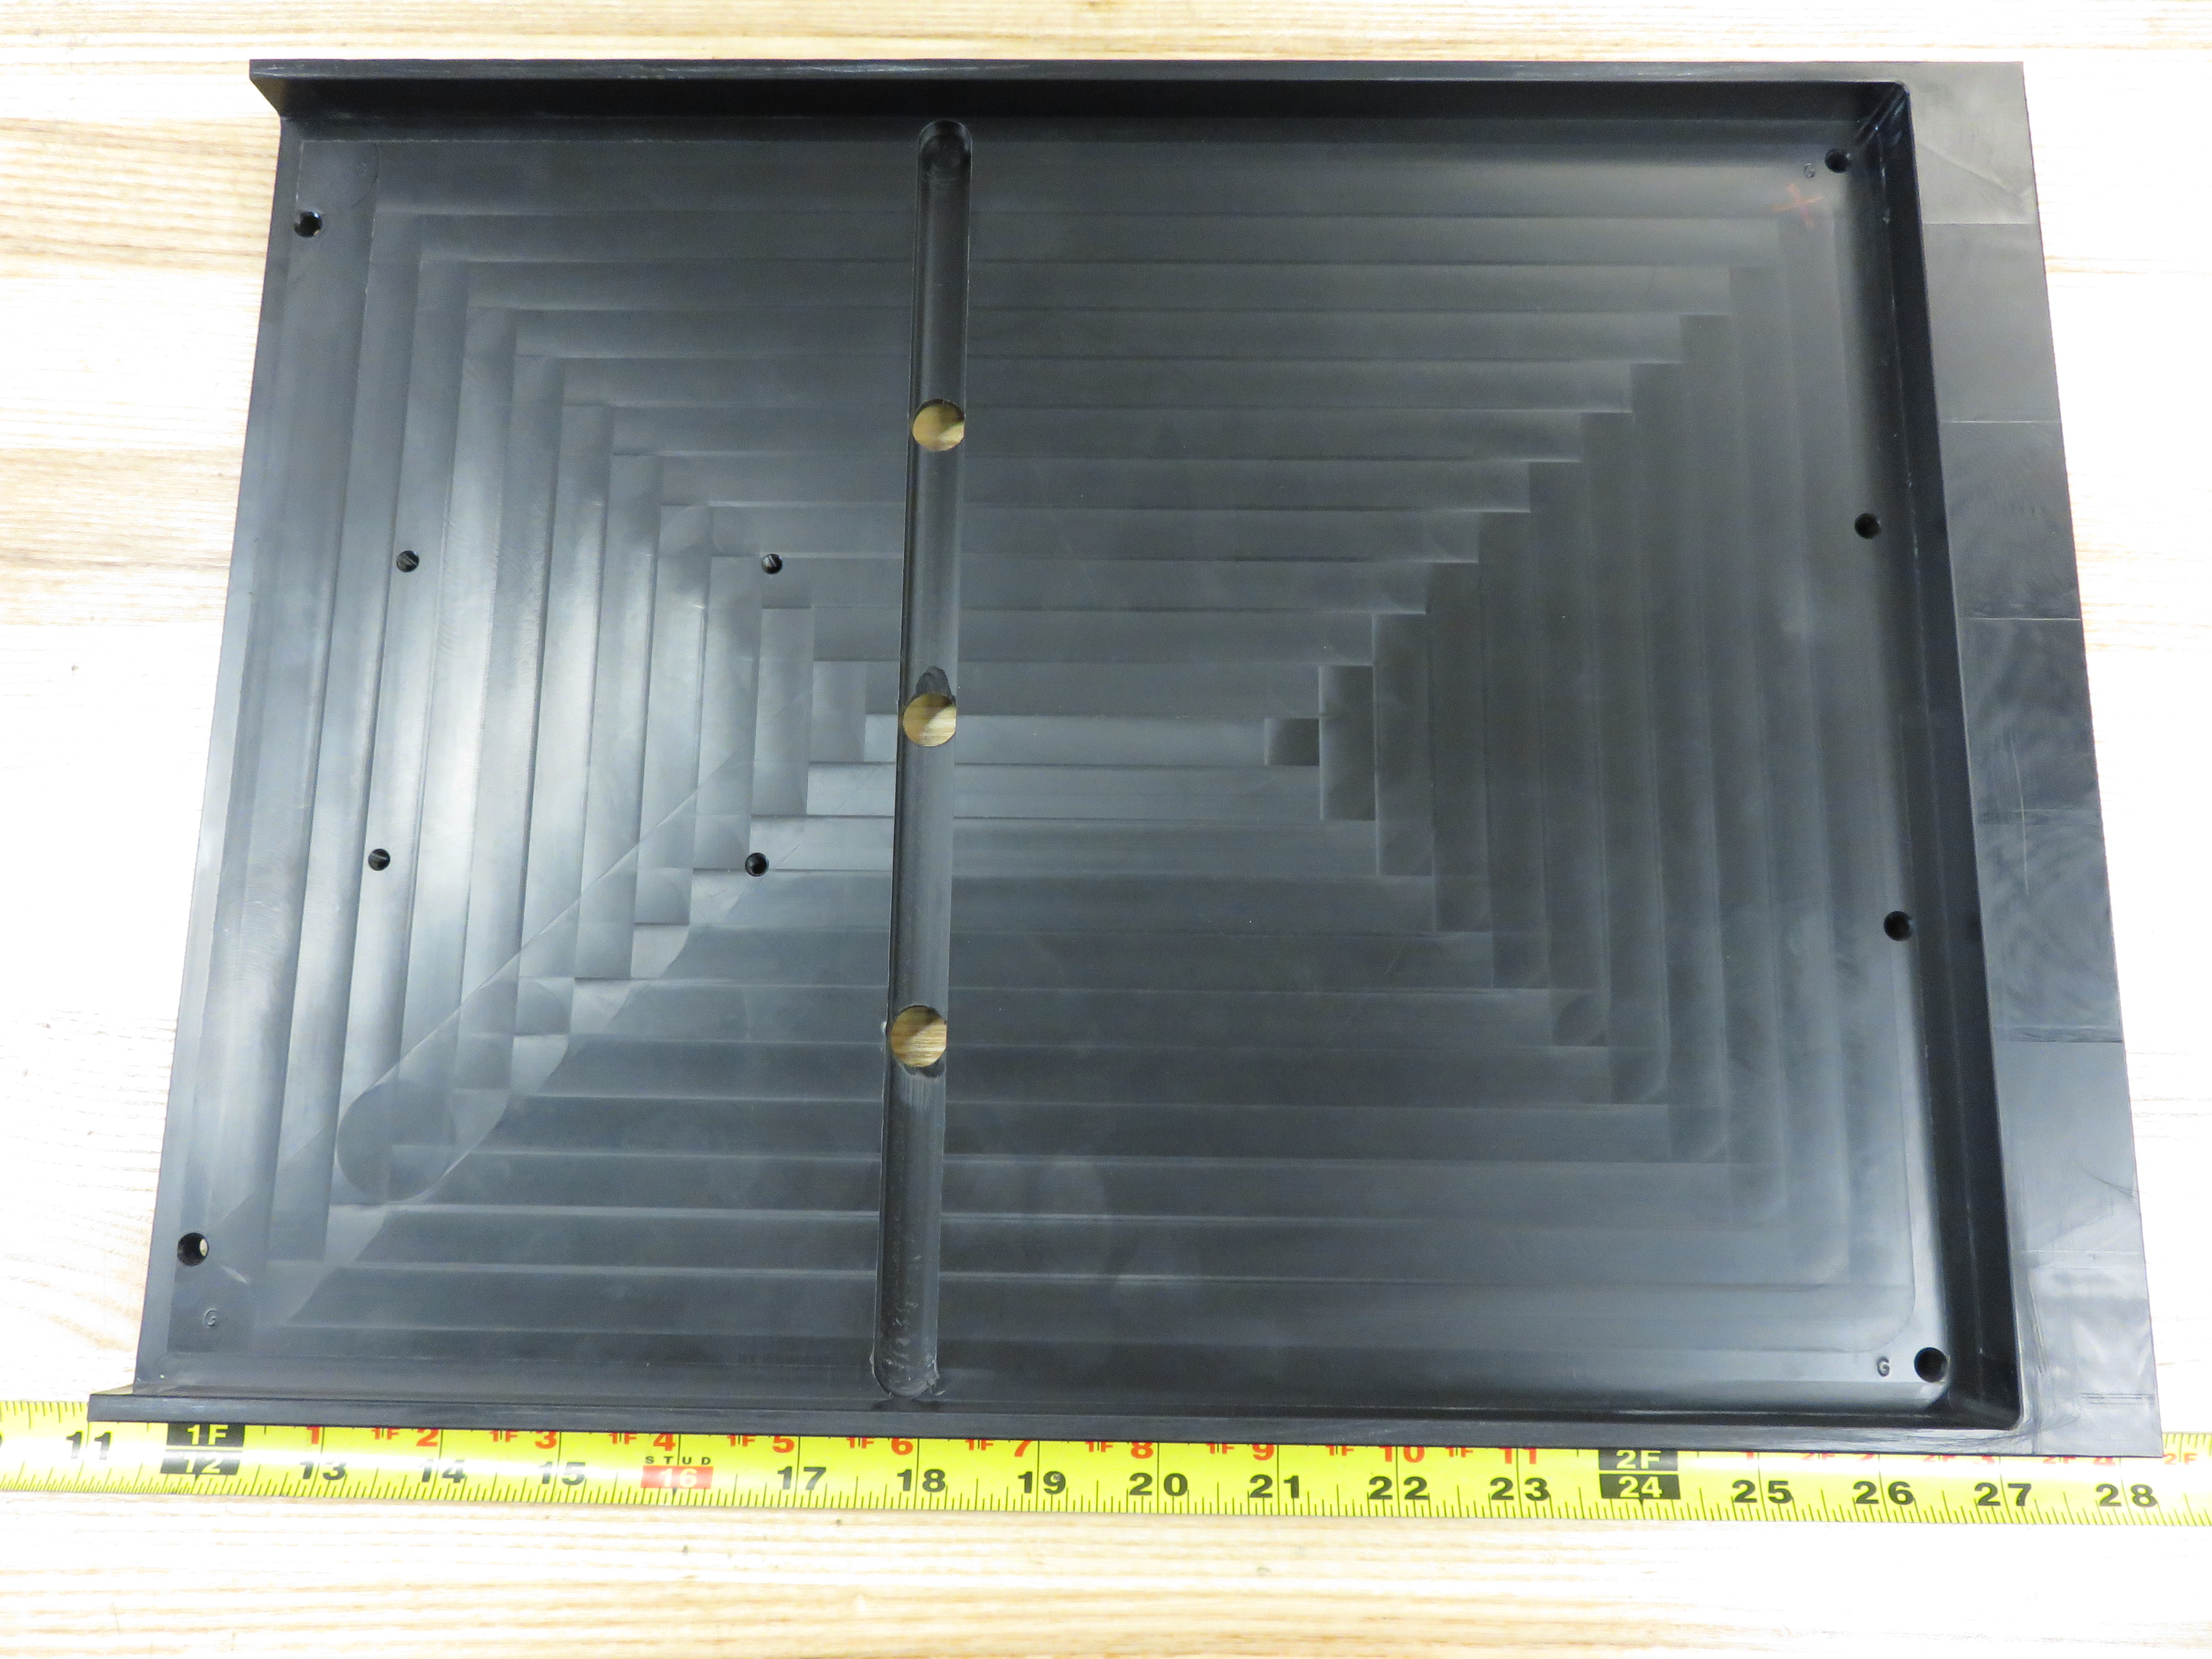
\includegraphics[scale=0.18]{facility/MachinedParts/G_meas_v2.JPG}
\caption{ \footnotesize part}
\end{figure}


%%%%%%%%%%%%%%%%%%%%%%%%%%%%%%%%%%%%%%
%%%%%%%%%%%%%%%%%%%%%%%%%%%%%%%%%%%%%%
\clearpage
\section{Assembly Procedure}

\begin{figure}[h!]
\centering
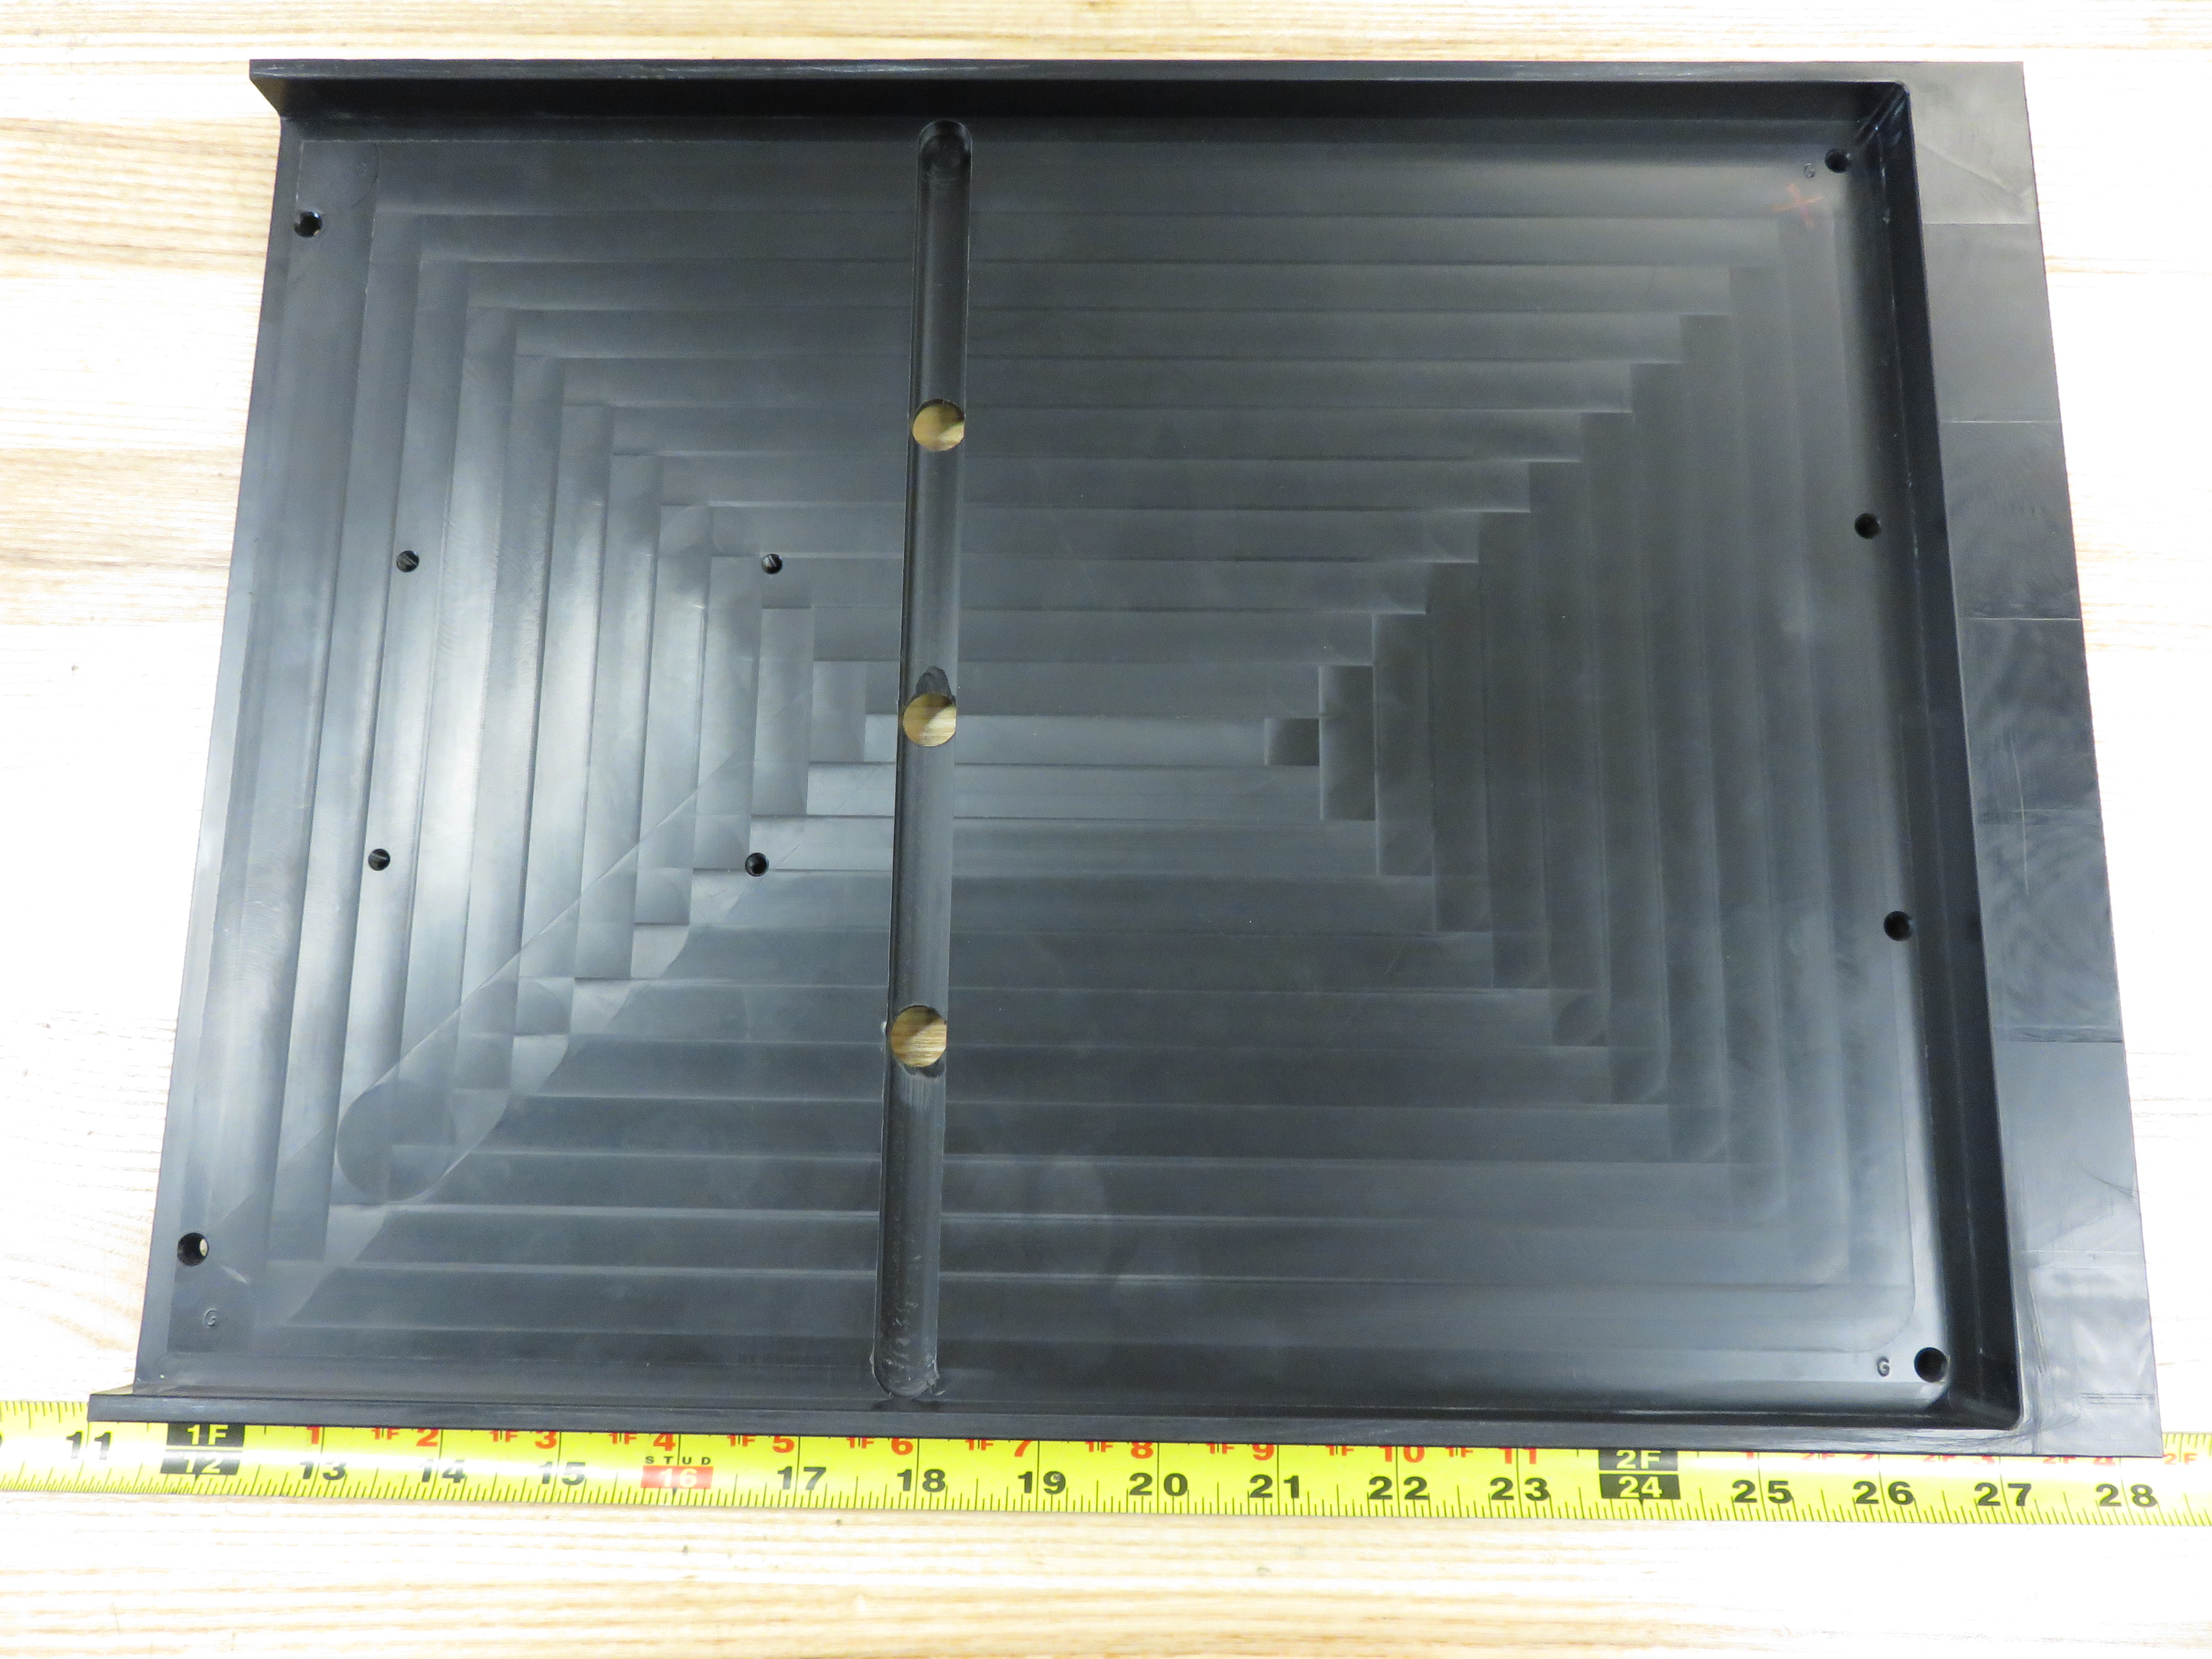
\includegraphics[scale=0.1]{facility/MachinedParts/G_meas_v2.JPG}
\caption{ \footnotesize part}
\label{fig:partsG}
\end{figure}